\documentclass[10pt,oneside]{book}

%%%%%%%%%%%%%%%%%
% import packages %
%%%%%%%%%%%%%%%%%
\usepackage{lipsum}
\usepackage{lmodern}
\usepackage{ragged2e}
\usepackage{adjustbox}
\usepackage{array}
\usepackage{rotating}
\usepackage{array}
\usepackage{setspace}
\usepackage{algorithm}
\usepackage{algpseudocode}
\usepackage{multirow}
\usepackage{booktabs}
\usepackage{makecell}
\usepackage{tcolorbox}
\usepackage{graphicx} 
\usepackage{fancybox} 
\usepackage{soul,color}
\usepackage{amsmath}
\usepackage{pdfpages}
\usepackage{tocloft}
\usepackage{amssymb}
\usepackage{tikz}
\usepackage{titlesec}
\usepackage{titletoc}
\usepackage{tabularx}
\usepackage{hyperref}
\usepackage{epigraph}
\usepackage{pdfpages}
\usepackage{pdflscape}
\usepackage{afterpage}
\usepackage{tablefootnote}
\usepackage{rotating}
\usepackage{pgfgantt}
\usepackage{multicol}
\usepackage{enumitem}
\usepackage{svg}
\usepackage{xcolor}
\usepackage[dvipsnames]{xcolor}

\usepackage[table]{xcolor}
\usepackage[acronyms]{glossaries}
\usepackage[
layout=letterpaper, 
paper=letterpaper, 
portrait, 
head=0.5in,
foot=0.5in,
top=.75in, 
bottom=.75in, 
left=0.75in, 
right=0.75in, 
margin=1in
]{geometry}
\usepackage[style=numeric-comp,backend=biber,backref=true,sorting=none]{biblatex}
\usepackage{cleveref}
\usepackage[toc,page]{appendix}
\usepackage{subfiles} % best loaded last in the preamble

% Custom column type for ragged-right with a fixed width
\newcolumntype{L}[1]{>{\raggedright\let\newline\\\arraybackslash\hspace{0pt}}m{#1}}

\makeglossaries
\definecolor{skyblue}{rgb}{0.529,0.808,0.922} % Adjust the values as desired
\definecolor{lightgreen}{rgb}{0.5647, 0.9333, 0.5647} % Adjust the values as desired
\definecolor{salmon}{rgb}{0.9804, 0.5020, 0.4471} % Adjust the values as desired
%Acronyms
\newacronym{tar}{TAR}{Technology-Assisted Review}
\newacronym{cal}{CAL}{Continuous Active Learning}
\newacronym{llm}{LLM}{Large Language Model}
\newacronym{gnn}{GNN}{Graph Neural Network}
\newacronym{gcn}{GCN}{Graph Convolutional Network}
\newacronym{gat}{GAT}{Graph Attention Networks}
\newacronym{bcs}{BCS}{Backwards Citation Searching}
\newacronym{fcs}{FCS}{Forwards Citation Searching}
\newacronym{ebm}{EBM}{Evidence-Based Medicine}
\newacronym{spl}{SPL}{Simple Passive Learning}
\newacronym{sal}{SAL}{Simple Passive Learning}
\newacronym{rct}{RCT}{Randomised Controlled Trial}
\newacronym{ir}{IR}{Information Retrieval}
\newacronym{tfidf}{TF-IDF}{Term Frequency-Inverse Document Frequency}
\newacronym{mlm}{MLM}{Masked Language Modelling}
\newacronym{cbrs}{CBRS}{Content-Based Recommendation System}
\newacronym{dta}{DTA}{Diagnostic Test Accuracy Reviews}
\newacronym{svm}{SVM}{Support Vector Machine}
\newacronym{bmi}{BMI}{Base Model Implementation}
\newacronym{bert}{BERT}{Bidirectional Encoder Representations from Transformers}
\newacronym{cdt}{CDT}{Centre for Doctoral Training}
\newacronym{clef}{CLEF}{Conference and Labs of the Evaluation Forum}
\newacronym{cnn}{CNN}{Convolutional Neural Network}
\newacronym{gpt}{GPT}{Generative Pre-trained Transformer}
\newacronym{nlp}{NLP}{Natural Language Processing}
\newacronym{ukri}{UKRI}{UK Research and Innovation}
\newacronym{prd}{PRD}{Percentage of Relevant Doocuments}
\newacronym{wssk}{WSS@k}{Work saved over sampling}

% %%%%%%%%%%%%%%%%%%%%%%%%%%%%%%%%%%%%%%%%%%
% % Other commands
% %%%%%%%%%%%%%%%%%%%%%%%%%%%%%%%%%%%%%%%%%%

\newcommand{\bibliographyLSR}[1]{\bibliography{#1}}
\newcommand{\ts}{\textsuperscript} %sobrescrito

\onehalfspacing

\AtBeginBibliography{\small}

\usetikzlibrary{shapes, arrows, positioning, fit,backgrounds}
\usetikzlibrary{arrows.meta}

\hypersetup{
colorlinks=true,
urlcolor=blue,
linkcolor=blue,
citecolor=blue,
pdftitle={@title - @author},
pdfsubject={Systematic Review},
pdfauthor={@author},
pdfkeywords={list; here; your; keywords (key words)}
}

\addbibresource{zot_references.bib}
\setlength{\cftsecnumwidth}{2.5em}
\setcounter{tocdepth}{1}
\begin{document}

\pagenumbering{arabic}

\begin{titlepage}


% -------------------------------------------------------------------
% You need to edit the details here
% -------------------------------------------------------------------

\begin{center}
{\LARGE University of Sheffield}\\[1.5cm]
\linespread{1.2}\huge {\bfseries Efficient Screening in Medical Systematic Reviews}\\[1.5cm]
\linespread{1}

\includegraphics[width=5cm]{Confirmation Review/images/tuoslogo.png}\\[1cm]
{\Large Dr. Aaron HA Fletcher}\\[1cm]
% {\large \emph{Supervisor:} Dr. Mark Stevenson}\\[1cm] % if applicable
\large A report submitted in partial fulfilment of the requirements\\ for the degree of PhD in Computer Science\\[0.3cm] 
\textit{in the}\\[0.3cm]
Department of Computer Science\\[2cm]
\today
\end{center}

\end{titlepage}

% -------------------------------------------------------------------
% Declaration
% -------------------------------------------------------------------

\newpage
\section*{\Large Declaration}

All sentences or passages quoted in this document from other people's work have been specifically acknowledged by clear cross-referencing to author, work and page(s).  Any illustrations that are not the work of the author of this report have been used with the explicit permission of the originator and are specifically acknowledged.  I understand that failure to do this amounts to plagiarism and will be considered grounds for failure.

The following are specifically replicated figure(s), grouped by license: 

\begin{itemize}
    \item Figure \ref{fig:increasing_publications_over_time} - CC BY-NC 4.0\footnote{\url{https://creativecommons.org/licenses/by-nc/4.0/}}
    \item Figures \ref{fig:prisma_flow}, \ref{fig:cochrane_ultrasound}, \ref{fig:pool_based_query} - CC BY 4.0 \footnote{\url{https://creativecommons.org/licenses/by/4.0/}}
    \item Figure \ref{fig:autotar_process} - In the Public Domain 
\end{itemize}

\vspace{20em}

\noindent Name: Aaron HA Fletcher\\[1mm]
\rule[1em]{25em}{0.5pt}

\noindent Signature:\\[1mm]
\rule[1em]{25em}{0.5pt}

\noindent Date:04/04/2025\\[1mm]
\rule[1em]{25em}{0.5pt}



%%%%%%%%%%%%
% Abstract %
%%%%%%%%%%%%
%% remove spacing from abstract

\chapter*{\Large \center Abstract}

% Guidance of how to write an abstract/summary provided by Nature: https://cbs.umn.edu/sites/cbs.umn.edu/files/public/downloads/Annotated_Nature_abstract.pdf

Systematic reviews are indispensable for evidence-based medicine but remain time-intensive and vulnerable to delays. As biomedical literature grows, conventional screening workflows become unsustainable. This research addresses these challenges by developing new Technology-Assisted Review (TAR) techniques that integrate richer metadata and relational signals, combined with flexible stopping rules. First, it uses citation network analysis—leveraging backwards and forwards references—to enhance early retrieval of critical studies and expand the training set for Continuous Active Learning (CAL). Second, it incorporates structured metadata (e.g., publication date, authorship, citation counts) into Graph Neural Networks to capture deeper inter-document relationships and improve prioritisation. Finally, it proposes utility-driven stopping criteria that move beyond fixed recall thresholds, focusing instead on how newly identified evidence shifts overall clinical conclusions. These methods will be evaluated on publicly available datasets such as CLEF-TAR and Synergy using metrics including recall@95\%, R-Precision, Work Saved over Sampling, and Percentage of Relevant Documents screened. By uniting novel ranking and stopping approaches, the research aims to substantially reduce screening workloads and accelerate high-quality, resource-efficient systematic reviews
    \smallskip
    \smallskip
    
    \textbf{Keywords} -  Systematic Reviews, Stopping Algorithms, Continuous Active Learning, Technology-Assisted Review, Utility, Medical Literature Screening, Evidence-based medicine, Metadata analysis
\newpage
\begingroup % Localize font size change
\small % Or \scriptsize or \tiny
\vspace*{-3cm}
\tableofcontents

\endgroup
% \listoffigures
% \listoftables
\newpage
\newcommand{\lightshadowbox}[1]{%
  \setlength{\fboxsep}{6pt}%
  \setlength{\shadowsize}{1pt}%
  \shadowbox{#1}%
}
\begin{multicols}{2}
\printglossary[type=\acronymtype]
\end{multicols}
\newpage
%%%%%%%%%%%
% Article %
%%%%%%%%%%%
\chapter{Executive Overview}

\epigraph{A man is known by the company he keeps}{Aesop}

\section{Background}
Systematic reviews are a cornerstone for \gls*{ebm}, providing rigorous, high-level research syntheses to guide clinical practice and policy. Yet this rigour carries a steep cost: systematic reviews are labour-intensive, often requiring researchers to screen thousands of documents manually. The problem this research aims to improve is efficiency in this process (i.e., the amount of documents screened). \gls*{tar} methods, particularly \gls*{cal}, promise to alleviate some of this burden; however, many existing approaches still treat documents as isolated entities, overlooking inter-document relationships or disregarding previously recalled documents' contribution to a search goal.

Better document representation can solve this problem. Just as an individual's quality might be inferred from their associations, the true value of a research document often lies not only in its isolated content but also in its connections to the broader scholarly landscape. Manual screening, and even many \gls*{cal} approaches, shallowly represent documents. That is to say, they use only information sourced from the title and abstract despite many more signals being available (inter-document connections), such as citation networks or metadata (e.g., source of publication, authorship, date of publication). These signals, used instinctively by human operators, could steer the selection for screening towards high-value studies. Moreover, the conventional practice of stopping screening relies on a simplistic, binary categorisation of documents as relevant or not, triggering the stop after a fixed ``target recall" threshold is met. This shallow document representation fails to recognise that documents contribute variably to a review's conclusions. While it provides a seemingly objective benchmark, target recall fails to consider the information's utility. Whether the accumulated evidence sufficiently addresses (i.e., how the information contained within a document relates to other documents) the research question or whether further screening will likely produce diminishing returns remains unexamined. 

This PhD, therefore, seeks more efficient and information-centric strategies to automate systematic review screening. First, this research will investigate relationship-aware \gls*{cal} methods that harness inter-document connections to rank and prioritise more intelligently for screening. Second, this research will examine the value of intra-document information, creating utility-driven stopping criteria that shift the focus from static recall targets to the actual value of newly discovered evidence. Rather than screen indiscriminately to meet a blanket recall requirement, the process stops once the reviewed studies collectively offer a robust answer to the research question. By utilising existing inter-document information or aligning the screening endpoint with genuine evidence needs, the resource demands of systematic reviews can be reduced while maintaining quality.


\section{Objectives and research questions}

The overarching goal is to reduce the manual screening workload (e.g., low \gls*{wssk}, \gls*{prd}) while maintaining key performance measures (e.g., high Recall@k, R-Precision).

To address this goal, both document screening prioritisation and stopping methods must be considered (see Sections~\ref{sec:screening Priorisation}, \ref{sec:metadata}, and \ref{sec:Stopping_algorithms}). Specifically, this PhD proposes improving the representation of documents in \gls*{cal} and aligning stopping methods with user information needs (see Section~\ref{sec:Project_Overview}). Three core research questions guide the work:

\begin{enumerate} 

\item \textbf{RQ 1}: \emph{What is the impact of integrating backwards and forward citation network analysis on the performance of \gls*{cal} models for medical systematic review screening?}
\item \textbf{RQ 2}: \emph{How does incorporating \gls*{gnn} architectures that utilize article metadata (e.g., publication date, author information, citation counts) affect the efficiency and accuracy of document prioritisation in \gls*{cal}, compared to traditional text-only representations?}
\item \textbf{RQ 3}: \emph{How do stopping criteria based on the utility of retrieved information (aligned with user information needs) influence the total manual screening workload in \gls*{cal}, and how do these criteria compare with conventional recall-based stopping rules?}

\end{enumerate}

These questions will be addressed using publicly available datasets such as \gls*{clef}-\gls*{tar} and Synergy, enriched with metadata from resources like OpenAlex (see Section~\ref{sec:datasets}). Experiments will employ existing approaches (e.g., Encoder-CAL, Baseline Model implementations) and introduce novel methods (e.g., utility-based stopping algorithms that factor in the implications of recalled information; see Section~\ref{sec:research_proposals}).

Ultimately, this PhD aims to develop methods that reduce the screening demands of systematic reviews. By combining better document representations through metadata or citation-aware insights and flexible stopping rules, the research seeks to make evidence synthesis more resource-efficient and timely in an era of exploding medical literature.

\chapter{Literature Review}

\section{Systematic reviews}

Systematic reviews provide a rigorous and transparent approach to synthesising research evidence on a specific topic, forming a cornerstone of evidence-based practice. Unlike traditional narrative reviews, systematic reviews adhere to a pre-defined, systematic methodology that minimises bias and ensures reproducibility. This methodical approach encompasses comprehensive literature searches, critical appraisal of studies, and careful synthesis of findings, ultimately providing a reliable and comprehensive overview of the current state of knowledge.

The term \emph{systematic} underscores the methodical and structured approach used throughout the review process. While the precise execution varies depending on the type of review and research question, several core characteristics define this methodology:

\begin{itemize}
    \item {\bf{Explicit, Step-by-Step Methodology:}} systematic reviews follow a clearly defined, step-by-step methodology, often documented in comprehensive procedural manuals. In medicine, for instance, the Cochrane Collaboration's Review Manual \cite{lefebvre_cochrane_2011} provides a detailed guide to conducting Cochrane Reviews. Similarly, in qualitative research, Noblit and Hare's book on meta-ethnography \cite{noblit_meta-ethnography_1988} outlines procedures for synthesising qualitative studies. These manuals provide a framework for standardised, transparent reviews.
    \item {\bf{Pre-Established Review Protocol:}} systematic reviews require the development of a detailed protocol {\it{before}} the review commences. This protocol acts as a blueprint, outlining the review's objectives, search strategy, inclusion and exclusion criteria, data extraction methods, and analysis plan. The pre-defined protocol prevents arbitrary changes in the review's scope during the process and minimises duplication of effort among reviewers. Furthermore, many reviewers register their protocols in publicly accessible registries like PROSPERO\footnote{https://www.crd.york.ac.uk/prospero/}, or open-access platforms, enhancing transparency and accountability \cite{tawfik_protocol_2020}.
    \item {\bf{Reporting Guidelines:}} systematic reviews adhere to established reporting guidelines to ensure clarity and consistency. These guidelines specify the essential elements to include in the final review report \cite{moher_preferred_2010}. Numerous reporting guidelines are available, tailored to various review types and research designs. Resources like the EQUATOR Network\footnote{https://www.equator-network.org/} compile and offer these guidelines, promoting standardised reporting across different fields.
    
    \item {\bf{Quality Assessment Checklist:}} The checklist provides an assessment of the methodological quality (risk of bias) of included studies, aiding the reader in interpreting the overall credibility of the review's findings. This allows the reader to answer the question, ``Is this a good or bad example of a review?". This process typically uses validated quality assessment checklists or tools appropriate for the study designs under review \cite{whiting_proposed_2017}.
    \item {\bf{Methodological Surveys or Audits:}} Methodological surveys or audits evaluate how emerging review types (e.g., scoping or umbrella reviews) are conducted, often signalling the need for refined reporting standards. They can occur before formal guidelines are established or continuously e.g., \cite{dalton_potential_2017, france_methodological_2014}. By aggregating practices from published reviews, they identify methodological inconsistencies (e.g., misuse of meta-analysis for heterogeneous data) or innovations. Such audits signal when a review type gains traction and inform consensus on best practices, often catalysing reporting standards (e.g., PRISMA extensions) or warnings against flawed approaches \cite{tricco_prisma_2018, sarkis-onofre_how_2021,rethlefsen_prisma-s_2021, rethlefsen_prisma-s_2021-1}
\end{itemize}

While this document explores the methodologies and challenges of systematic reviews, its literature review, constrained by the typical limitations of a PhD project, cannot be a full systematic review because systematic reviews are resource-intensive, often requiring dedicated funding, a multi-year timeframe, and a multidisciplinary team.
\subsection{In medicine}

% systematic review use in medicine.
Central to medical research and practice, systematic reviews synthesise existing literature on clearly framed clinical questions \cite{kranke_evidence-based_2010, higgins_cochrane_2019}. They consolidate extensive evidence into a cohesive, critically appraised summary that offers clear decision support for clinicians and policymakers. systematic reviews are created across virtually every medical sub-specialty. Recent publications illustrate their scope, exploring cardiovascular risks in endometriosis \cite{parsa_endometriosis_2025}, clarifying links between antidepressants and insomnia in adolescents \cite{turkmen_systematic_2025}, and examining anaemia in pregnancy \cite{azzam_anemia_2025}. The exponential growth of new studies necessitates reliance on systematic syntheses for reliable, up-to-date guidance.


% How systematic reviews support decision making
Systematic reviews provide the highest-ranked evidence for many clinical questions in \gls*{ebm} underpinning clinical decision-making. As shown in Table \ref{tab:evidence_levels}, \gls*{ebm} organises evidence types hierarchically, ranking expert opinion as the weakest (level 5) and systematic reviews of \glspl*{rct} as the strongest (level 1a). To minimise bias, systematic reviews, unlike traditional narrative reviews, follow strict methodological guidelines such as comprehensive literature searches and critical appraisal of each included study. This rigorous approach ensures a transparent and reproducible evidence synthesis, enabling practitioners to make more informed decisions tailored to patient needs.

\begin{table}[ht]
\centering
\small
\begin{adjustbox}{width=\columnwidth/2}
\begin{tabular}{|c|l|}
\hline
\textbf{Level} & \textbf{Type of Evidence} \\
\hline
1a & Systematic reviews of randomised controlled trials \\
1b & Individual randomized controlled trials \\
2a & Systematic reviews of cohort studies \\
2b & Individual cohort studies \\
3a & Systematic reviews of case-control studies \\
3b & Individual case-control studies \\
4 & Case series \\
5 & Expert opinion \\
\hline
\end{tabular}
\end{adjustbox}
\caption[A summarised form of the 2009 OCEBM Levels of Evidence]{A summarised form of the 2009 OCEBM Levels of Evidence \cite{noauthor_oxford_nodate} There are conflicting thoughts on the absolute ranking of strength for all evidence sources \cite{swanson_how_2010, guyatt_grade_2008}; however, a key commonality is that systematic reviews (of \glspl*{rct}) are considered the strongest evidence type.}
\label{tab:evidence_levels}
\end{table}

% Growth of systematic reviews
\begin{figure}
    \centering
    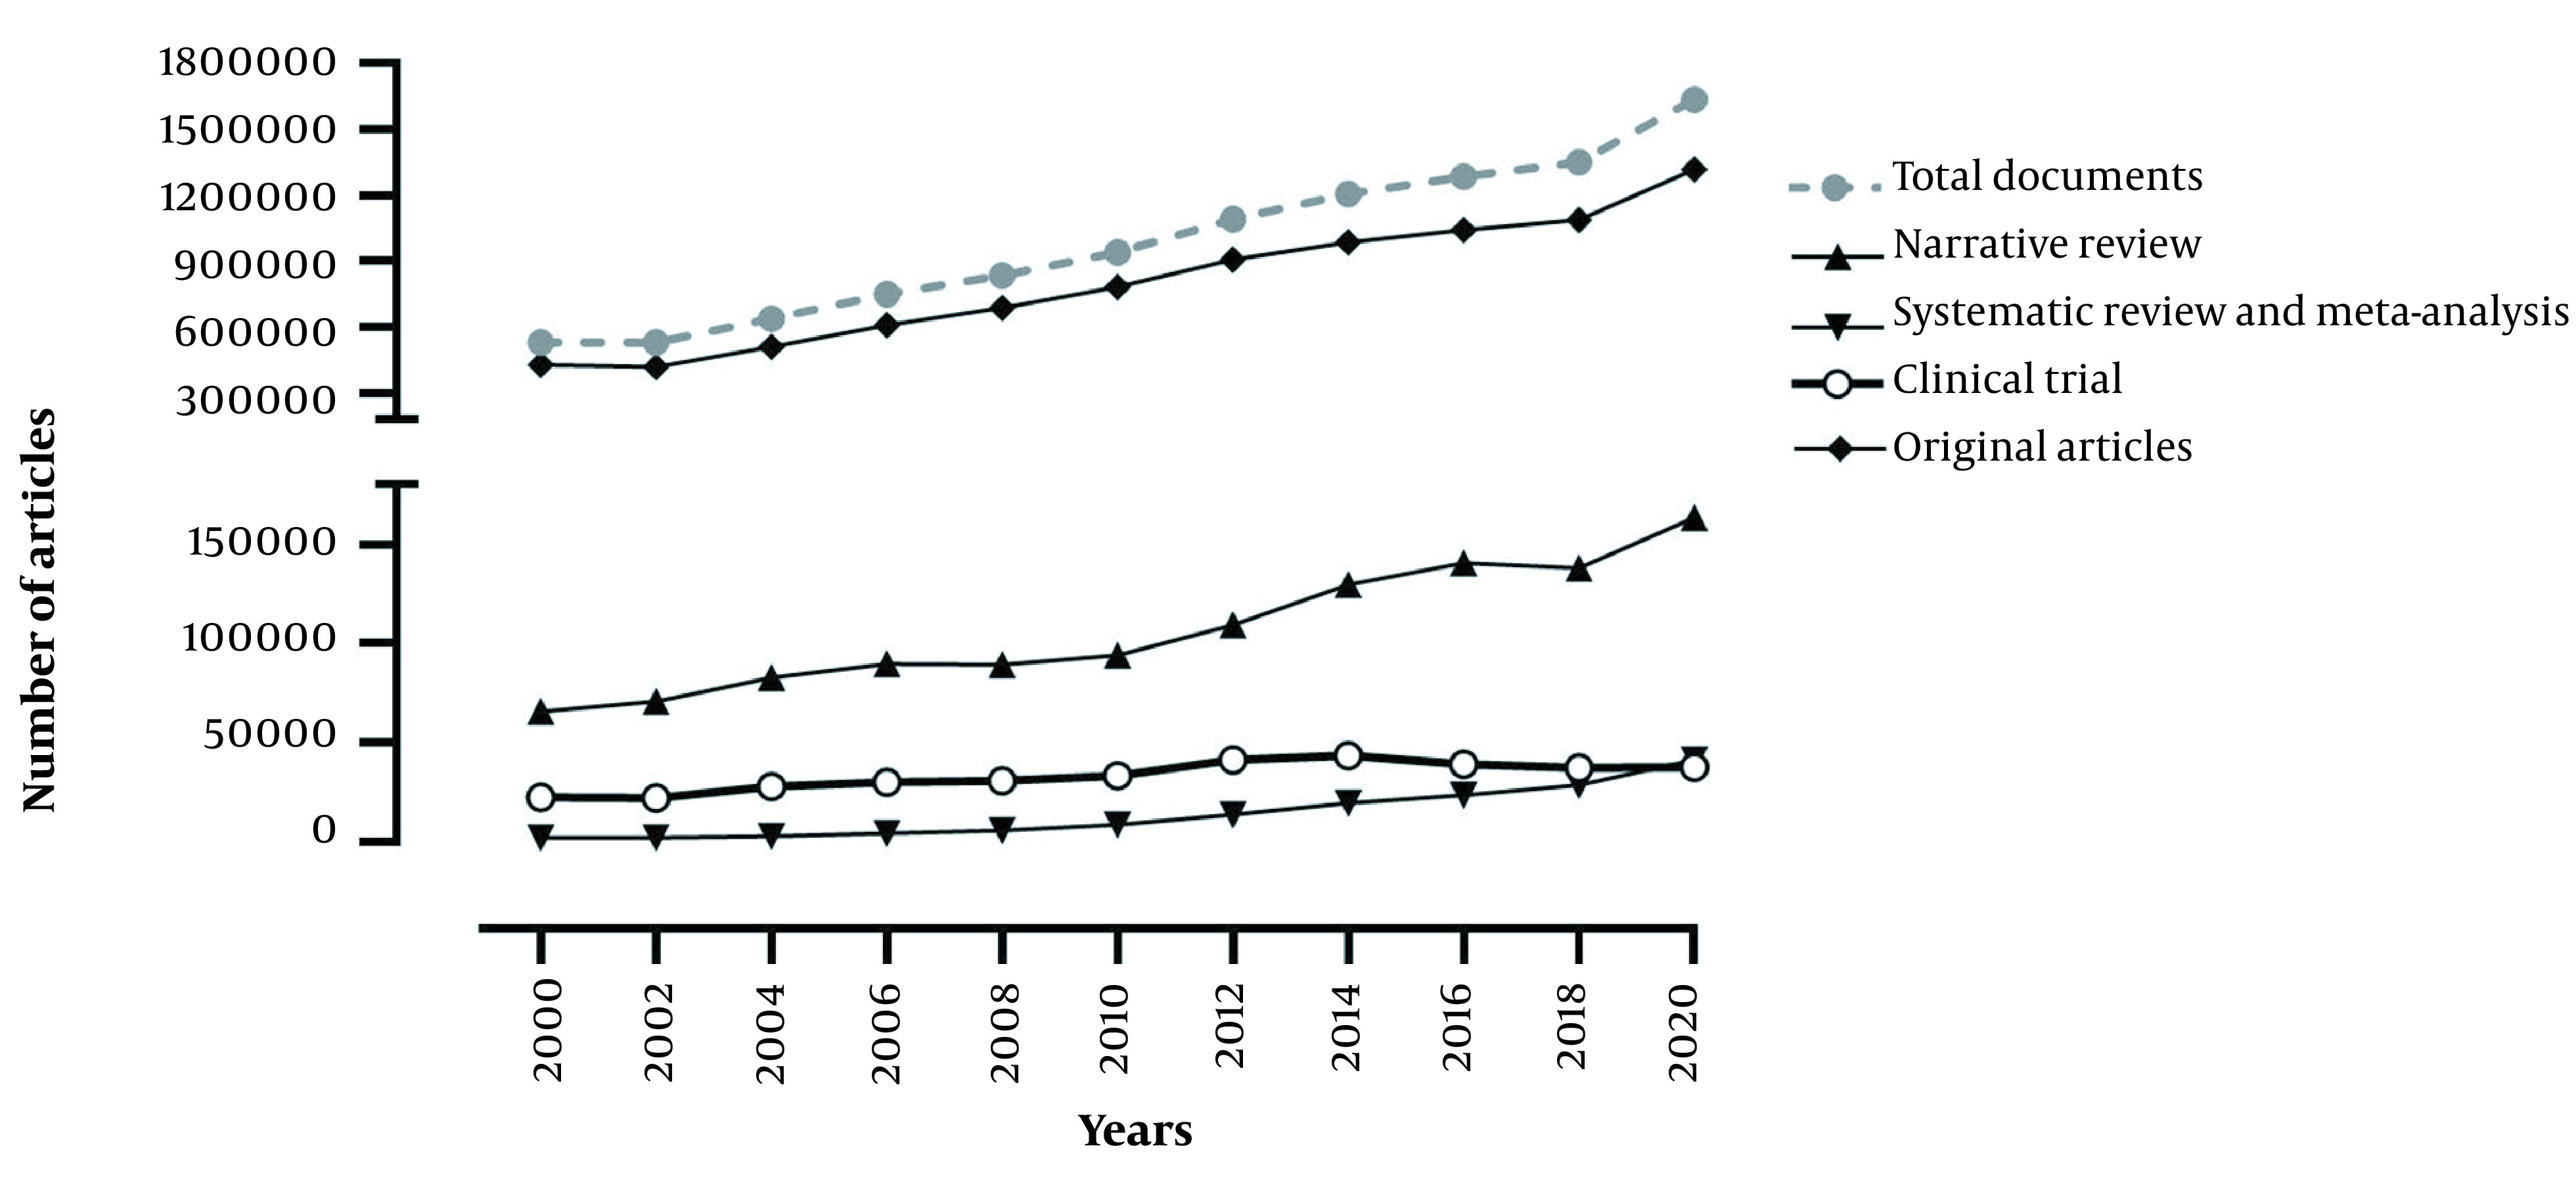
\includegraphics[width=1\linewidth]{Confirmation Review/images/increase_in_publications.jpg}
    \caption{Increasing publications over the past two decades \cite{ghasemi_scientific_2022}.\protect\footnotemark}
    \label{fig:increasing_publications_over_time}
\end{figure}
\footnotetext{Reproduced from \cite{ghasemi_scientific_2022} under the CC BY-NC 4.0 license \url{https://creativecommons.org/licenses/by-nc/4.0/}. No changes were made. Noncommercial use only.}

The publication rate of systematic reviews in medicine has surged exponentially in recent decades, a trend reflecting their growing centrality to evidence-based practice. Between 1986 and 2015, PubMed indexed a 2,728\% increase in articles labelled as systematic reviews, far outpacing the 153\% rise in other publications during the same period \cite{ioannidis_mass_2016}. This expansion underscores a growing need for consolidated, high-quality evidence to address diverse clinical questions, especially as the volume of primary research increases. For instance, the number of clinical trials—a key source of evidence—doubled between 2001 and 2020, while peer-reviewed journals nearly tripled \cite{ghasemi_scientific_2022}; see Figure \ref{fig:increasing_publications_over_time}). Methodological advances, such as PRISMA guidelines and GRADE frameworks, have strengthened systematic review rigour, enabling them to shape clinical guidelines, inform policy, and even synthesise overlapping evidence through umbrella reviews. Cochrane exemplifies this impact: its 9,000+ systematic reviews, accessed over 17.5 million times by 2023, underscore its global reach and influence, reflected in a journal impact factor of 8.8\footnote{https://www.cochrane.org/about-us/scientific-strategy}.


\subsection{The process}

% Brief overview of the Cochrane Review process and its characteristics.
No single universally correct process for conducting a medical systematic review exists, with various approaches available (e.g., Joanna Briggs Institute review~\cite{santos_joanna_2018}, Meta-Analysis~\cite{moher_improving_1999} Network Meta-Analysis~\cite{bafeta_reporting_2014} or Cochrane Review~\cite{cipriani_what_2011, munn_what_2018}). 

The Cochrane Review framework is particularly interesting for computer science because each step is meticulously documented~\cite{guyatt_grade_2008, cumpston_chapter_2024}, which, along with their abundance, enables potential automation. Broadly, a Cochrane systematic review undergoes five steps: question framing, identifying relevant work, quality assessment, summarisation and interpretation, as shown in Table \ref{tab:stages_of_systematic review}. The ``identifying relevant work" phase iteratively narrows down a large document pool until only eligible documents remain, with this process often being visualised within the final review itself in a PRISMA flow diagram (Figure \ref{fig:prisma_flow}). There are multiple procedures within the ``Identifying Relevant Work" phase, yet a single substage called ``Title and Abstract screening" commands 10-20\% of the time it takes to plan and conduct an entire systematic review~\cite{haddaway_predicting_2019}, making it a prime target for efficiency improvements. 

\begin{figure}
    \centering
    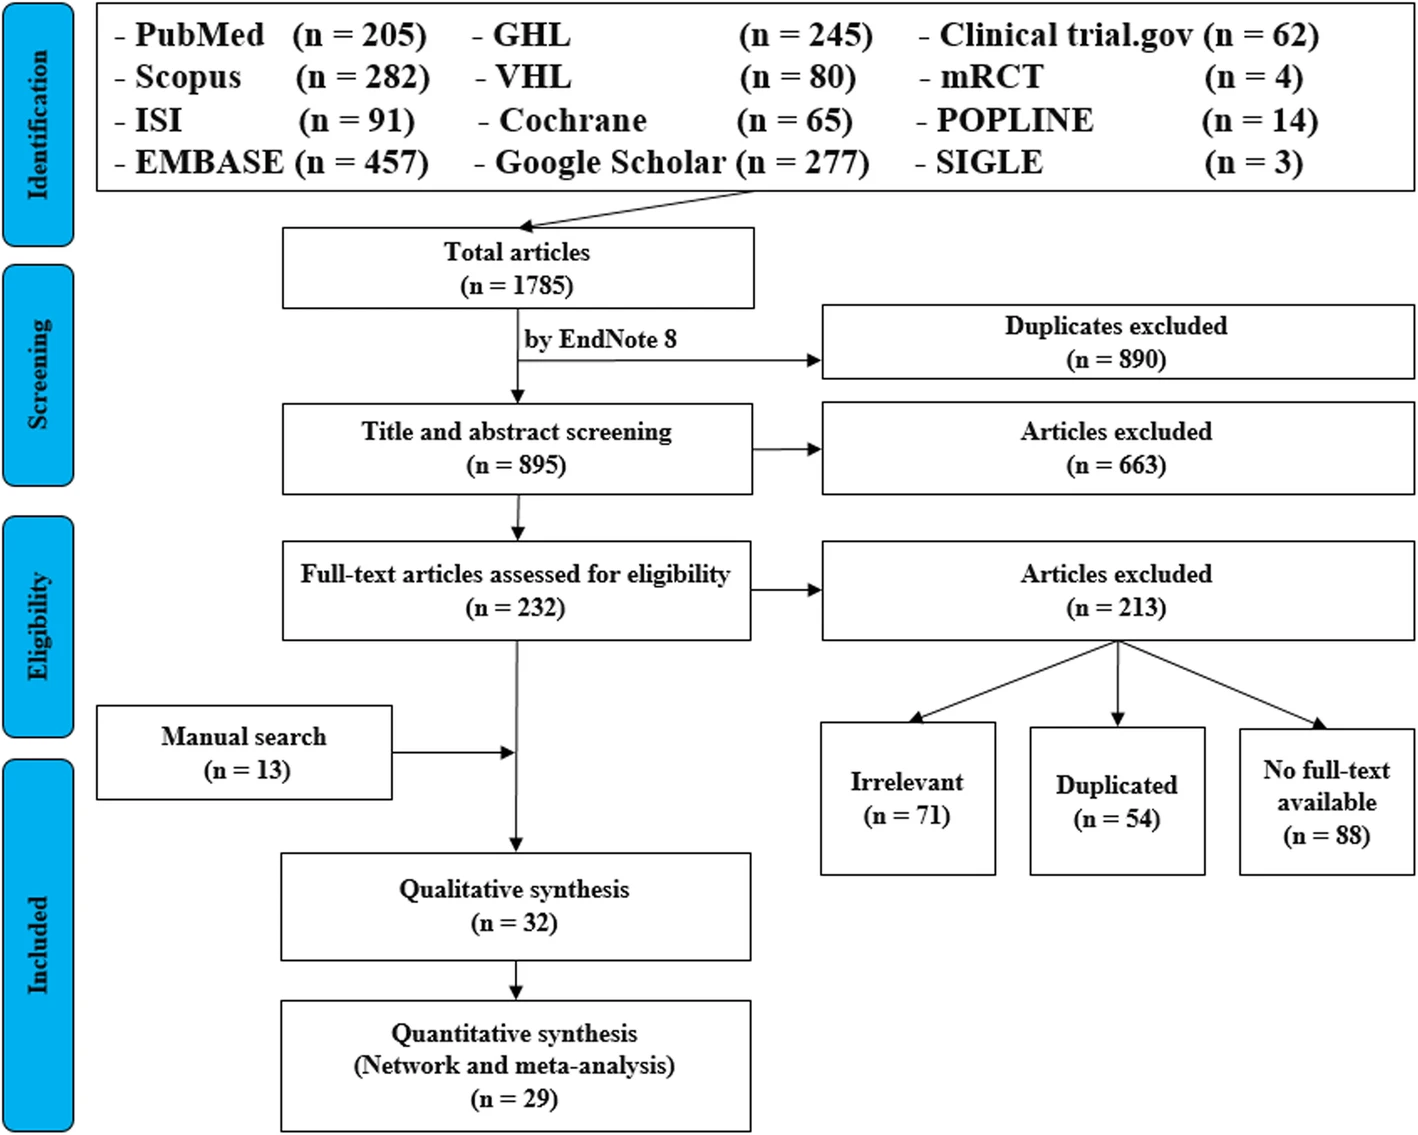
\includegraphics[width=1\linewidth]{Confirmation Review//images/prisma_flow.png}
    \caption{PRISMA flow diagram for a simulated Cochrane systematic review \cite{tawfik_protocol_2020}. Note the different substages of the identification of relevant work in blue.\protect\footnotemark}
    \label{fig:prisma_flow}
\end{figure}
\footnotetext{Reproduced from \cite{tawfik_protocol_2020} under the CC BY 4.0 license \url{https://creativecommons.org/licenses/by/4.0/}. No changes were made.}


To further understand the ``Identifying relevant work" stage, consider the PRISMA flow diagram for a recent systematic review~\cite{tawfik_protocol_2020}. An identification stage compiles all potential studies from searched databases into a large dataset of studies that may or may not be relevant to the systematic review, $n=1785$. Screening further refines this pool by removing duplicates and assessing titles and abstracts to reduce the number of full-text articles requiring assessment in the eligibility substage, $n=895$. This is traditionally achieved through 2-3 reviewers manually evaluating titles and abstracts to determine whether each study should be included or excluded based on predetermined criteria. At this stage, studies are typically categorised as relevant (related to the systematic review) or not relevant (unrelated to the systematic review) and passed to the full-text eligibility assessment.

% This stage can be further granularised into several substages, many of which directly involve the tasks outlined above:

% \begin{itemize}
% \item {\bf{Inclusion/exclusion criteria generation:}} Defining the precise criteria for including or excluding studies, supported by \gls*{ir} specialist guidance on source selection and search strategy development.
% \item {\bf{Search Strategy Development:}} Creating the detailed search algorithms used to query databases (a core \gls*{ir} specialist responsibility).
% \item {\bf{Database Searching:}} Implementing the search strategy across various databases and trial registers (conducted by \gls*{ir} specialists).
% \item {\bf{Protocol Writing:}} Documenting the search methodology in detail, with \gls*{ir} specialists contributing the search methods section.
% \item {\bf{Title and Abstract Screening:}} Initially assessing study relevance based on titles and abstracts, facilitated by \gls*{ir} specialist results management and de-duplication.
% \item {\bf{Full-Text Download and Screening:}} Obtaining and reviewing the full text of potentially relevant studies supported by \gls*{ir} specialist document retrieval.
% \item {\bf{Manual Search:}} Supplementing database searches with manual searching of relevant journals, conference proceedings, and other sources, often guided by \gls*{ir} specialists.
% \end{itemize}



\begin{table*}[t]
\centering
\small
\begin{tabular}{|c|p{0.85\textwidth}|}
\hline
\textbf{Stage} & \textbf{Purpose} \\
\hline
1 & \textbf{Question Framing:} The research question is structured and explicitly formulated. \\\hline
2 & \textbf{Identifying relevant work:} A wide range of databases are searched to identify research to be included. Potential research is first identified, screened, and eligibility checked, and then a decision is made on including that research \cite{tawfik_step_2019}. \\\hline
3 & \textbf{Quality Assessment:} Research is tested for quality, such as minimum research design, and subjected to higher quality assessment checks, including tests for research heterogeneity. \\\hline
4 & \textbf{Summarisation:} Data synthesis occurs with tabulation of study characteristics and quality. Statistical testing is performed at this stage. \\\hline
5 & \textbf{Interpretation:} Any issues highlighted in the previous steps should be addressed. Generate recommendations guided by reference to the strength of the evidence. \\
\hline
\end{tabular}
\caption{Stages of a Systematic Review.}
\label{tab:stages_of_systematic review}
\end{table*}

% % Focus on the title and abstract screening substage.
% This PhD research focuses on the Title and Abstract screening substage of the `Identifying Relevant Work' phase, a critical process often visualised using the PRISMA flow diagram (Figure \ref{fig:prisma_flow}). This stage alone is estimated to account for 10-20\% of the time it takes to plan and conduct a systematic review \cite{haddaway_predicting_2019}.

% Research within the title and abstract screening substage

% Best practices for traditional title and abstract screening have been outlined to increase consistency and reduce bias in the title and abstract screening phase \cite{polanin_best_2019}.

% At the start of this stage, using an abstract screening tool with clear, concise questions and conducting training sessions where screeners learn and pilot test the screening process using 20-30 abstracts is recommended to ensure intercoder agreement. During the screening phase, teams should hold weekly meetings, avoid changes to the screening tool, use text-mining, employ independent double-screening of each work, and immediately reconcile disputes. After the screening phase, analysing the process itself for validity is recommended.

Research on title and abstract screening reveals crucial elements for successful outcomes and strongly supports using both the title \emph{and} abstract. For instance, recent work comparing title-only (Ti/O) versus title-plus-abstract (Ti+Ab) screening found that Ti+Ab achieved significantly higher sensitivity (94.7\% vs. 57.9\%) by capturing studies with ambiguous titles but relevant abstract content. At the same time, Ti/O risked excluding 42.1\% of eligible studies due to insufficient title clarity~\cite{teo_title-plus-abstract_2023}. Another study showed that adopting a Title-First screening approach (rejecting a study based on the title, followed by abstract assessment for inclusion) reduced workload compared to a title-and-abstract approach, with no reduction in recall of relevant research~\cite{mateen_titles_2013}.

% The use of non-experts (medical students) as a feasible alternative to experts when undertaking citation screening was demonstrated in the TASER study \cite{ng_title_2014}.

\subsection{Challenges}

Systematic reviews in medicine commonly strive for near-total recall (e.g., 95\% or more) before concluding the title and abstract screening phase. However, there is no guarantee that screening beyond a certain point meaningfully changes a review's clinical or scientific conclusions. Such ``over-screening" can exhaust finite reviewer resources, inflate costs 
thereby reducing efficiency \cite{prabha_what_2007, ilani_analysis_2024}. 

% Resource usage
A crucial challenge in undertaking a systematic review is efficiency. The title and abstract screening stage often involves hundreds or thousands of potentially relevant studies, each requiring assessment by at least one, ideally two, trained reviewers. This scale is not trivial. Estimates suggest that a proficient information specialist can screen between 0.133 and 2.88 abstracts per minute \cite{shemilt_use_2016,giummarra_evaluation_2020,felizardo_visual_2013}; consequently, screening a large volume of abstracts is a significant undertaking. This task's sheer scale demands considerable time from expert reviewers, whose expertise is costly and scarce, thus increasing the financial burden of conducting systematic reviews

Furthermore, attempts to mitigate costs by reducing screening requirements, such as employing a single reviewer, substantially compromise the recall of relevant studies. \glspl*{rct} using the Cochrane Crowd platform demonstrated that single-reviewer approaches could miss up to 13\% of relevant studies, whereas a dual-reviewer approach missed only 3\% \cite{gartlehner_single-reviewer_2020}. Similar findings have been reported in other studies, indicating that even experienced reviewers, when working in isolation, consistently missed more relevant references \cite{waffenschmidt_single_2019}. Because minimising the risk of excluding pertinent evidence is crucial, dual screening is considered indispensable despite the associated resource implications. The use of non-experts (medical students) was demonstrated to be a feasible alternative to experts when undertaking citation screening, as shown in the TASER study \cite{ng_title_2014}.

The temporal demands of systematic reviews are also substantial, with an average completion time of 67.3 weeks \cite{borah_analysis_2017}. The screening phase alone can prolong the timeline by several months. While the precise number of abstracts screened per review is not uniformly documented, surveys of established systematic reviews report a median of 555 abstracts, spanning from 232 to 9,648 \cite{nama_successful_2021}. In one analysis of 14 systematic reviews, 19,334 abstracts were screened, yielding only 3.1\% (605) relevant studies \cite{nama_successful_2021}. At such scales, reviewer fatigue poses a legitimate concern, as prolonged engagement in tedious screening tasks can diminish vigilance and compromise the accuracy of the review process.


% % Consistency 
% Consistently applying inclusion and exclusion criteria across all studies poses a persistent challenge, with inter-coder discrepancies common, even when two reviewers evaluate the same abstracts. This is particularly true for studies in a ``grey area" that require nuanced judgment for inclusion or exclusion. Resolving these discrepancies typically requires discussion between reviewers or consultation with a third, adding roughly 5 minutes per conflict \cite{shemilt_use_2016}. With thousands of abstracts, this resolution process significantly increases resource and time demands. Moreover, inherent variability within review teams—differing expertise, subjective interpretations, and individual biases—fosters inconsistencies. Although rigorous pilot testing and ongoing calibration exercises help, consistently applying criteria remains challenging, especially over extended screening periods with numerous abstracts.

% % Bias
% Bias in title and abstract screening occurs when certain studies are systematically favoured or excluded. Several factors contribute to this risk: 
% \begin{itemize} 
% \item \textbf{Single-reviewer bias:} As previously discussed, single-reviewer approaches miss more eligible studies, potentially reducing the comprehensiveness of the final evidence base.
% \item \textbf{User fatigue:} Extended screening periods can cause ``attention drift", leading reviewers to exclude relevant studies inadvertently.
% \item \textbf{Prior knowledge and expectations:} Reviewers with pre-existing knowledge may unconsciously favour studies aligning with their beliefs or published in well-regarded journals. Conversely, they may dismiss studies they deem less relevant, introducing selection bias.
% \end{itemize}

% % Bias Ctd
% Another source of bias is assuming humans always label documents correctly. Wang et al. report error rates as high as 10.76\% during abstract screening \cite{wang_error_2020}. While strategies like dual-review and reporting inter-coder agreements help, they do not guarantee error elimination.
 
\section{Screening prioritisation}\label{sec:screening Priorisation}

%What is screening prioritisation
Screening prioritisation is an approach to improve efficiency in the title and abstract screening phase of systematic reviews. Screening prioritisation is the process of ranking documents by their likelihood of relevance. Prioritisation puts the documents at the top of the list that should address the systematic review's research question, enabling reviewers to find relevant literature more quickly. In principle, prioritisation can dramatically reduce screening efforts by allowing a screener to stop once they have recalled most or all of the relevant articles. For example, consider a hypothetical dataset of 20 documents, with 5 of those being relevant. All 20 must be screened without any prioritisation to find the five that matter. If the documents are ranked perfectly in descending order of relevance, the screener could theoretically recall all five relevant documents by examining only the first 5 in the list, reducing total document reviews. 

\gls*{tar}, also known as Computer-Assisted Review or Predictive Coding, is a process that uses machine learning to assist in document screening. Approaches to \gls*{tar} fall into two categories: (1) those ranking directly with queries (e.g. the query being the title \cite{alharbi_ranking_2017, alharbi_retrieving_2018}, boolean search terms  \cite{alharbi_ranking_2017, alharbi_retrieving_2018, alharbi_ranking_2019}, or review objectives \cite{ferro_qut_2017, scells_integrating_2017}), and (2) those using indirect methods like relevance feedback \cite{alharbi_ranking_2019} or active learning \cite{cormack_technology-assisted_2017, cormack_systems_2019, grossman_technology-assisted_2010, grossman_automatic_2017}. This research focuses on using active learning, which has successfully been used in many areas of \gls*{ir} \cite{cormack_autonomy_2015, cormack_engineering_2016, yu_fast2_2019, yu_finding_2018, miwa_reducing_2014}.

\subsection{Active learning}

% What is active learning
Deep learning models and other classifiers often require large labelled datasets to perform well. In systematic review screening, gathering labels can be slow and expensive, especially at the outset when little is known about relevance. Active learning aims to mitigate this challenge by selecting the most \emph{informative} unlabelled documents for human labelling in iterative cycles.

This iterative process aims to substantially improve model performance while minimising the time and effort required for labelling. A typical active learning workflow selects a batch of unlabelled samples based on their potential to improve the model. These selected samples are then labelled and incorporated into the growing training dataset. The model is subsequently retrained using this expanded dataset, leading to improved model classification and ranking accuracy. The core principle behind active learning is to balance exploring uncertain or ambiguous documents (exploration) and exploiting documents that are likely to be highly relevant (exploitation). This approach enhances the model's ability to rank documents accurately, making the systematic review process more efficient and effective.

Variations of active learning exist, such as membership query synthesis \cite{angluin_queries_1988}, stream-based selective \cite{akinseloyin_novel_2024} and pool-based sampling \cite{lewis_sequential_1994}. 
Pool-based sampling best suits title and abstract screening because the unlabelled document set is known in advance. Figure \ref{fig:pool_based_query} illustrates this workflow. Mainstream prioritisation approaches largely model documents based on their text alone, such as bag-of-words or embeddings of titles and abstracts \cite{diao_lexical_2021}. Conventional active learning algorithms do not incorporate inter-document relationships; they rely on textual features or basic metadata to measure uncertainty and relevance. This can overlook important ``network-level" cues (e.g., shared references, reciprocal citations, co-authorship clusters) that could guide the active learning process toward the most pertinent articles faster.


\begin{figure}
\centering
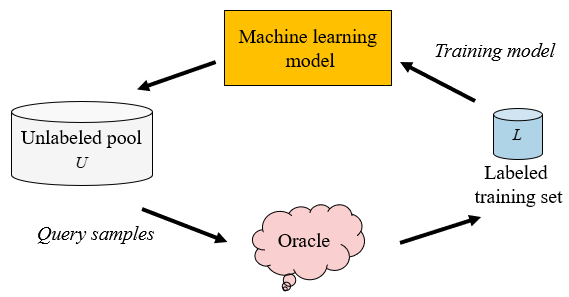
\includegraphics[width=0.5\linewidth]{Confirmation Review/images/pool_based_strategy.png}
\caption{Overview of a pool-based query strategy for active learning. \cite{ren_survey_2020}\protect\footnotemark}.
\label{fig:pool_based_query}
\end{figure}
\footnotetext{Reproduced from \cite{ren_survey_2020} under the CC BY 4.0 license \url{https://creativecommons.org/licenses/by/4.0/}. No changes were made.}


% Active Learning Notation 
\begin{tcolorbox}[title=The General Active Learning Process]  
\small
The active learning process can be formally described as follows:

\begin{enumerate}
    \item A sampling policy ($\pi$) intelligently selects the most informative samples ($\mathbf{T}_{C,i}$) from an unlabelled dataset ($\mathbf{T}_{U,i}$).
    \item These samples are passed to an oracle ($O$) for labelling.
    \item The labelled samples are added to a growing known dataset ($\mathbf{T}_{K,i}$).
    \item A classifier is trained on this labelled dataset.
    \item The classifier ranks the remaining unlabelled samples in ($\mathbf{T}_{U,i}$), often based on the classifier's uncertainty or expected model improvement.
    \item This iterative process repeats, intending to improve the classifier's performance with each labelling round until a predefined stopping criterion is met.
\end{enumerate}
\end{tcolorbox}
The oracle within systematic reviews denotes a human-verified label resulting from screening potential research for inclusion within the systematic review within the title and abstract screening stage. More concretely, $O$ can be considered a function $O(x) = y$ where $x$ is a document representation (i.e. if a human was reviewing a title and abstract or a representation of the title and abstract for automated approaches), and $y$ is the assigned category (included or excluded). In active learning research, in contrast to research in systematic reviews, it is assumed that for each $x$, $O$ provides a single judgement ($y$), which is always correct.


\begin{table*}[t]
    \centering
    \footnotesize

    \begin{tabular}{|c|c|>{\raggedright\arraybackslash}p{11cm}|}
        \hline
        \textbf{Notation}    & \textbf{Explanation}                            & \textbf{Notes}                                                                                \\
        \hline
        \(\textbf{T}\)       & Total dataset                                   & e.g. Research gathered after Identification phase of the selection process.                   \\
        \hline
        \(i\)                & Iteration                                       & A single cycle within the active learning process.                                            \\
        \hline
        \(\textbf{T}_{K,i}\) & Known datapoints per iteration                  & e.g. research that has been screened by a reviewer                                            \\
        \hline
        \(\textbf{T}_{U,i}\) & Unknown datapoints per iteration                & e.g. research that has not been screened by a reviewer                                        \\
        \hline
        \(\textbf{T}_{C,i}\) & A subset of \(\textbf{T}_{U,i}\) to be labelled & chosen by a policy, datapoints to be screened by a reviewer.                                  \\
        \hline
        $\pi$                & Policy                                          & How \(\textbf{T}_{U,i}\) is selected, e.g. uncertainty, random, certainty, diversity sampling \\
        \hline
        O                    & Oracle                                          & Often a domain expert, who assigns labels to unscreened research.                             \\
        \hline
        \(T_R\)              & Total Relevant Documents                        & All research that should be included in a systematic review.                                  \\
        \hline
        \(T_{IR}\)           & Total Irrelevant Documents                      & All research that should not be included in a systematic review.                              \\
        \hline
    \end{tabular}
    \caption{Notation used for active learning within this review}
    \label{tab:notation}
\end{table*}


% How AL doesn't address systematic review issues

While active learning offers advantages, its direct application to systematic reviews has limitations:

\begin{itemize}
    \item \textbf{Delayed Incorporation of Early Information:} Waiting until a minimum number of documents has been assessed before training the model means valuable information gathered in the early phases is not incorporated into the ranking process.
    \item \textbf{Delayed Search Phase:} The actual search and screening process is delayed until sufficient relevant studies are present in the document collection.
    \item \textbf{Minimum Number of Relevant Studies Required:} A minimum number of relevant studies is often required in the initial document collection. This is usually impractical in the early stages of a systematic review.
\end{itemize}

To truly minimise screening effort, a scenario is needed where minimal expert screening is performed on documents returned from the identification phase, and the model can safely extrapolate that screening to a larger pool.

These disadvantages lead to diversifying \gls*{tar} approaches. The different \gls*{tar} approaches have been outlined in Table \ref{tab:differences_in_tar} and can be categorised as follows: \gls*{spl} \cite{cohen_reducing_2006}, where a ``seed set" of human-labelled documents from $T$ creates the labelled set $T_{K,i}$ used to train a classifier. This classifier then labels $T_{U, i}$ without further learning. \gls*{sal}, where a ``seed set" of human-labelled documents from $T$ creates the labelled set $T_{K,i}$ is used to train a classifier. This classifier then labels $T_{U, i}$, which is ordered by relevance, and then the most uncertain document labels are revealed. The model is retrained after each batch of newly labelled documents, improving its accuracy. The \gls*{cal} process is similar to SAL; the model is updated continuously, in real-time or near real-time, as human reviewers label documents. There are no discrete rounds; learning is ongoing. The system may still prioritise documents for review based on uncertainty or other strategies, but it can also adapt to reviewer behaviour and potentially re-rank documents on the fly. Cormack et al. \cite{cormack_autonomy_2015} argue that \gls*{cal} better aligns with systematic review workflows because the goal is to unearth all relevant documents quickly (i.e. exploitation) rather than just optimising model accuracy per see (i.e. balancing exploitation \emph{and} exploration). Nonetheless, as the subsequent research will show, \gls*{cal} approaches have traditionally treated each document individually rather than utilising the relational structure in the corpus.


\begin{table*}[t]

    \centering
    \footnotesize
    \begin{tabular}{|c|c|c|c|}
        \hline
        \textbf{Feature} & \textbf{\gls*{spl}} & \textbf{\gls*{sal}} & \textbf{\gls*{cal}} \\
        \hline
        Learning & One-time, from initial set  & Iterative, in batches  & Continuos, real-time \\
        \hline
        Model Updates & None after initial training & After each batch & After each labelled document \\
        \hline
        Reviewer Interaction & None after initial set & Periodic (batch-wise) & Continuous \\
        \hline
        Adaptability & Static  & Moderate & High \\
        \hline
        Prioritisation & Based on initial model & Adapts per batch & Adapts continuously \\
        \hline
    \end{tabular}
    \caption{The key differences between the different forms of active learning within \gls*{tar}.}
    \label{tab:differences_in_tar}
\end{table*}



\subsection{Metadata usage in screening}

% Clarify what is meant by metadata, and where we can find it!
\gls*{cal}, in principle, benefits greatly from additional signals that can quickly surface the most relevant documents. Citation networks and metadata can do exactly that. Within this research, metadata refers to the structured or semi-structured information accompanying a publication beyond its raw text—such as author affiliations, publication dates, co-author relationships, journal or conference venues, keywords (including MeSH terms), and other bibliographic details. This metadata is abundant, freely available, and already computed. OpenAlex\footnote{https://www.openalex.org}, for example, is an open-sourced API that covers a large proportion of the literature, providing extensive metadata.

Inter-document relationship refers to citation network analysis, which can be performed using this metadata. So, for example, if a paper cites another, this document is said to be related. Analysis of inter-document relationships and metadata is something that searchers instinctively do when screening documents. To illustrate, if a searcher finds a foundational relevant document, such as Cormack's work on Auto \gls*{tar}, their other work is likely related to that topic. If a searcher is searching for research on COVID-19, publications before 2019 are not likely to be related. 

The manual approach to title and abstract screening reviews all documents within the total document pool, so inter-document relationships offer little benefit. Interestingly, \gls*{bcs} and \gls*{fcs} are used in the Cochrane approach in the preceding stage, ``identification" that forms the pool~\cite{briscoe_conduct_2020, noauthor_mecir_nodate}. Once the pool of candidate articles is set, the screening phase—where documents are prioritised or ranked—almost always relies solely on each document’s title/abstract, ignoring citation or co-authorship signals that might refine relevance scores. This standard approach—extracting only an article’s abstract and minimal bibliographic fields—overlooks valuable signals embedded in established citation networks, co-author clusters, and publication venues.

Despite the substantial research on automating systematic review screening, most approaches rely almost exclusively on a document’s title and abstract (rarely supplemented with keywords or MeSH terms). A recent scoping review of PubMed-indexed studies on systematic review automation (covering 123 articles) demonstrates this gap clearly: Tóth et al. found that the great majority of record-screening automation tools (broadly utilising \gls*{spl}, \gls*{cal} or \gls*{spl} approaches) used either bag-of-words or \gls*{tfidf} representations of the title and abstract text, with only a small proportion incorporating additional metadata such as publication date or author information \cite{toth_automation_2024}. Indeed, a typical pipeline in these tools converts the abstract into a vector of token counts or embeddings and then applies a machine learning classifier or an active learning framework to predict relevance. While a handful of studies appended ``bibliographic details” or ``MeSH terms,” Tóth et al. note that these uses of metadata are inconsistent, rarely extend beyond indexing keywords and do not systematically exploit inter-document relationships (e.g., citation networks, co-authorship, or shared references). The author has not identified studies that incorporate metadata into \gls*{cal} in a structured way. 

Addressing this gap represents both a challenge and a major opportunity. Incorporating structured metadata into \gls*{cal} prioritisation pipelines could improve recall by surfacing relevant clusters of connected documents earlier. Simultaneously, it may reduce screening workloads by deprioritising documents in low-yield regions of the citation or co-authorship graph. Thus, research into \gls*{cal} here is viewed through the lens of how they represent documents and if they consider inter-document relationships.  

\subsection{\gls*{cal} for systematic reviews}

Recall targets in systematic reviews differ from other domains (e.g.\ e-discovery in law or social-media sentiment analysis) by demanding near-complete recall to ensure no critical study is missed. In medical research, overlooking even a single relevant article can critically affect the interpretation of evidence. Despite this demanding requirement, \gls*{cal} has shown promise for reducing systematic review screening workloads by up to 77\%~\cite{van_der_vet_propagation_2016}. Nonetheless, current \gls*{cal} approaches for systematic reviews still largely treat documents as stand-alone entities, relying on shallow representations (e.g.\ bag-of-words or simple neural embeddings) and giving limited attention to inter-document relationships (e.g.\ shared citations or authorship).

To understand the evolution of \gls*{cal} methods and identify opportunities for incorporating relational signals, the author categorises existing approaches based on how they represent documents (i.e., feature-based vs \ encoder-based vs \ decoder-based). A Feature-based approach is where the title and abstract are transformed into numerical vectors representing features like word presence or importance (e.g., \gls*{tfidf}); an Encoder-based approach, where models like \gls*{bert} capture semantic relationships between words in the title and abstract using a self-attention mechanism; and a Decoder-based approach is where generative models like \glspl*{gpt} predict the probability distribution of the next word in a sequence, leveraging unidirectional context. Such a taxonomy helps illustrate the progression from methods relying on simple lexical features to those capturing increasingly complex semantic relationships and ultimately highlights the potential for incorporating relational information.

\paragraph{Feature-based approaches:}
These methods, while foundational, represent documents as isolated entities. They typically transform document text (title and abstract) into numerical vectors, where each dimension represents a specific feature, such as the frequency of a term (e.g., \gls*{tfidf}). A common characteristic of these methods is their treatment of documents as relatively independent entities, focusing primarily on word-level importance without explicitly modelling the inter-document relationship.

Cormack et al.~\cite{cormack_evaluation_2014} introduced a foundational feature-based \gls*{cal} approach using a \gls*{svm} classifier. Their method trained a \gls*{svm} classifier on an initial set of documents identified through keyword seeding. While this work demonstrated the superiority of \gls*{cal} over traditional screening methods in an e-discovery context, it presented limitations when applied to the specific requirements of systematic reviews. Notably, the use of a large, fixed batch size (1,000 documents) and a focus on achieving recall@75\% are not well-aligned with the need for near-total recall and adaptive learning in medical literature reviews. Moreover, no leveraging of relational structure inherent in medical literature was used.

While subsequent research, like Auto~\gls*{tar}~\cite{cormack_autonomy_2015}, explored refinements such as alternative term weighting (e.g., Cornell ltc) and batch size optimisation, these methods still primarily focus on word-level importance within individual documents; Auto~\gls*{tar} approach is outlined in Figure~\ref{fig:autotar_process}. Auto~\gls*{tar} differed from the foundational system by using a single seed document (instead of 1,000) and incrementally increasing by approximately 10\% each iteration, rounded up, demonstrating improved performance and better alignment with systematic review screening. It used Cornell ltc term weighting \cite{salton_smart_1965} to represent documents. Auto~\gls*{tar} has remained a de facto baseline in many \gls*{cal} studies, sometimes called the \gls*{bmi}.

\begin{figure}
    \centering
    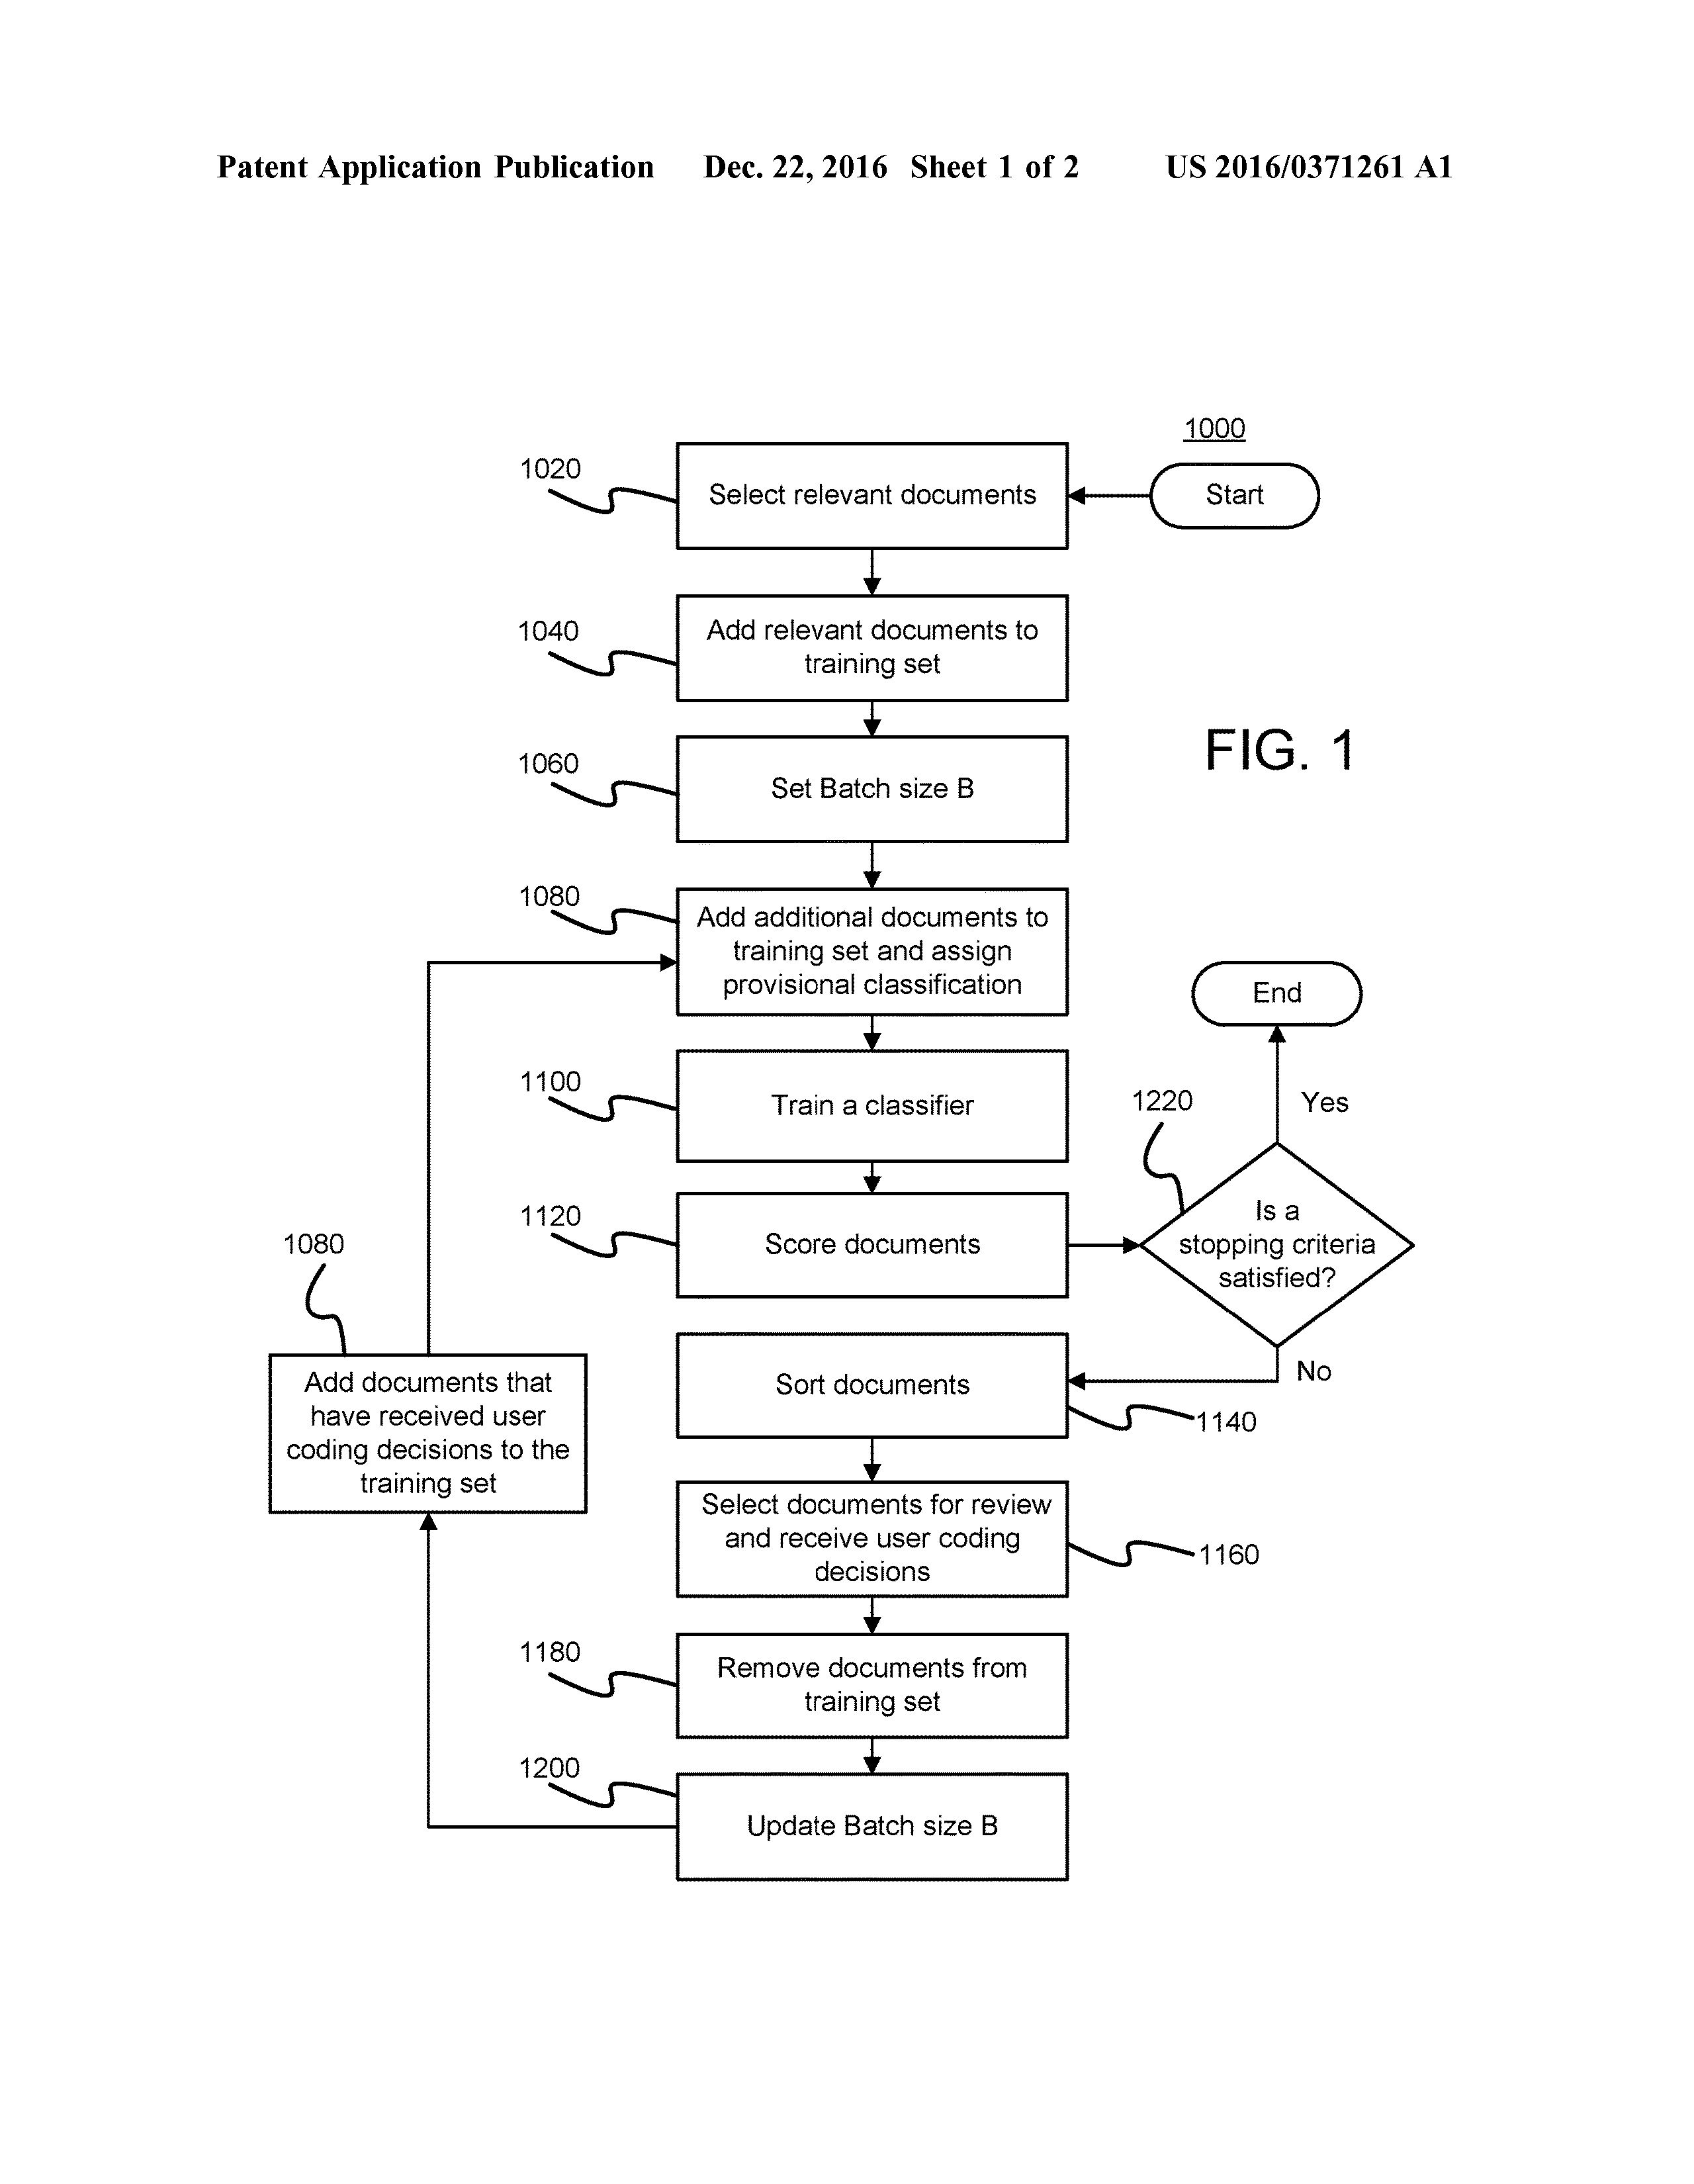
\includegraphics[width=0.95\linewidth]{Confirmation Review/images/autotar.jpg}
    \caption{Auto~\gls*{tar} outline, as documented within the patient filing by Cormack et al. \cite{cormack_systems_2016}\protect\footnotemark}.
    \label{fig:autotar_process}
\end{figure}

\footnotetext{\cite{cormack_systems_2016} Patents are in the public domain, and no license is required. No changes were made.}

More recent work has examined hyperparameter choices within feature-based \gls*{cal} pipelines. Ferdinands et al.~\cite{ferdinands_performance_2023} simulated human reviewers screening six labelled systematic reviews, comparing four classifiers (Naive Bayes, Logistic Regression, \gls*{svm}, Random Forest) under two document representations (\gls*{tfidf} vs.\ doc2vec). The results indicated that Naive Bayes with \gls*{tfidf} features reduced the average time to discovery. However, none of these systems integrated metadata or inter-document relationships.

% Approach looking at sentence-level classification vs document-level
Incorporating more information in the screening stage is a step towards richer representations, but they fail to leverage inter-document relationships fully. Although standard feature-based \gls*{cal} often relies on the title and abstract alone, Zhang et al.~\cite{zhang_evaluating_2020} showed that using isolated representative sentences (via a \gls*{tfidf}-based approach) could achieve comparable accuracy and higher efficiency than the \gls*{bmi}. These experiments did not use medical domain datasets and utilised full-text documents, but the study hints at the potential gains from more nuanced feature engineering. Other work has examined MeSH keywords \cite{miwa_reducing_2014} and Latent Dirichlet Allocation (LDA) \cite{hashimoto_topic_2016, miwa_reducing_2014} to enrich feature sets and showed promising performance improvements. This work demonstrates the potential for exploring alternative, superior representations beyond titles and abstracts.

% Incorporating semi-supervision via label propagation
Through incorporating citation proximity, Kontonatsios et al.'s work on label propagation highlights the potential of relational information ~\cite{kontonatsios_semi-supervised_2017}. It introduced a label-propagation method in which a small batch of human-labelled abstracts assign provisional labels (in \gls*{tfidf} or spectral-embedded space) to nearby unlabelled citations. These pseudo-labelled documents augment the training pool, accelerating the active learning process. The approach surfaced relevant papers significantly earlier than purely supervised strategies — reinforcing the notion of leveraging unlabelled data and relational signals (e.g.\ local neighbourhoods in feature space) to increase recall. Kontonatsios et al.’s results enhanced recall without imposing an additional annotation burden. This motivates further exploration of semi-supervised paradigms in future \gls*{cal} systems, especially with advanced document embeddings and network-based relationships.

% Summary of feature-based CAL
In summary, feature-based \gls*{cal} has proven robust and is a strong baseline.  However, these methods view documents as isolated or rely only on limited textual features (TF, \gls*{tfidf}, or keywords). \emph{They do not exploit deeper semantic embeddings or intricate inter-document relationships}, leaving a clear research gap. Though these feature-based techniques paved the way for \gls*{cal} in systematic reviews, they typically ignore nuanced contextual signals among documents. This omission impedes refined strategies for prioritising and terminating screening. The next section explores whether encoder-based methods offer a deeper representation — and possibly an avenue to more context-aware \gls*{cal}.

\paragraph{Encoder-based approaches:}
Encoder-based models like \gls*{bert} capture deeper semantic relationships within documents but typically do not explicitly model relationships between documents. Self-attention mechanisms have revolutionised the field of \gls*{nlp}, significantly improving performance across a wide range of tasks \cite{vaswani_attention_2023}. However, \gls*{cal} processes did not fully leverage these advancements initially. The major contribution of self-attention lies in its ability to generate context-dependent text representations, allowing for a more nuanced understanding of text compared to earlier feature-based methods. This capability enables self-attention models to capture subtle semantic relationships and long-range dependencies often missed by traditional approaches like \gls*{tfidf}, which were previously dominant in \gls*{tar}.

Encoder-based models, such as \gls*{bert}, PubMedBERT and BiolinkBERT, achieve high performance on classification tasks through a two-step process of pre-training (where a model has initially trained large corpora of text to develop a general understanding of language and the specific domain) and fine-tuning (where a pre-trained model is further trained on small,task-specific datasets to adapt it for the particular task). 

Initial work like CALBERT explored incorporating encoder-based models but did not demonstrate superiority \cite{sadri_continuous_2022}. CALBERT ranks a pool of documents using a logistic-regression-based–based \gls*{cal} model, then refines the top $k$ documents with a \gls*{bert}-based reranker. Each selected document (title + abstract) is truncated to 512 tokens, converted into an embedding via \glspl*{bert}  CLS token, and passed through a fully connected layer to produce a relevance score. After presenting the highest-scoring document for user feedback, CALBERT is fine-tuned on this new relevance information, and the underlying \gls*{cal} model is also retrained. However, despite the appeal of using transformers for feature-rich document representations, CALBERT often underperforms the simpler \gls*{bmi}. Variations such as appending the query text (monoBERT) or continuously fine-tuning \gls*{bert} did not yield consistent gains in a high-recall setting. 

Further research explored pre-training strategies that hindered encoder-based \gls*{cal}. Yang et al. \cite{yang_goldilocks_2022} fine-tuned a pre-trained \gls*{bert} on an unlabelled corpus (testing 0-10 epochs) before applying it to \gls*{cal}. They iteratively sampled 200 documents, labelled them, and fine-tuned \gls*{bert} for 20 epochs, using the previous iteration's model as the starting point. They found that five epochs of initial fine-tuning yielded performance comparable to \gls*{tfidf} and logistic regression on an in-domain dataset but significantly worse on an out-of-domain dataset. This could be attributed to ``catastrophic forgetting" \cite{xu_forget_2020}, where excessive fine-tuning on the task corpus causes the model to lose general knowledge from pre-training. However, Mao's subsequent research suggested that the optimal pre-training epoch (coined ``goldilocks" epoch) \gls*{cal} was not universal, especially in medical datasets \cite{mao_reproducibility_2024}. Mao's most performant model was not fine-tuned, but rather a model that uses a graph-based approach to pretrain, ${\text{BiolinkBERT}}_{\text{base}}$.

BioLinkBERT incorporates citation links during pre-training and represents a significant step towards leveraging relational information. It is the most performant encoder model on the \gls*{clef} dataset in a \gls*{cal} setting to date. The LinkBERT approach to pre-training models was to view a pertaining corpus as a graph of documents, with each document being a vertex and hyperlinks forming edges between documents \cite{yasunaga_linkbert_2022} and compared to \gls*{bert} approach in Figure \ref{fig:linkbert-comparison}. These linked documents were then placed within the same context, different from that of \gls*{bert} random document allocation, in which no linkage between documents within a context window is required. LinkBERT differs from curriculum learning, where a model is provided with examples of increasing difficulty, as the context windows' documents are not ordered by difficulty. A domain-specific variant of LinkBERT, BioLinkBERT\footnote{https://huggingface.co/michiyasunaga/BioLinkBERT-base}, was created, which was pre-trained only on PubMed articles, with linkage of documents being determined through citations of that research. Models were then trained using standard \gls*{mlm} and next-sentence prediction. The performance of a base model (100M parameters) and a large model (340M parameters) was compared to PubMedBERT\footnote{https://huggingface.co/microsoft/BiomedNLP-BiomedBERT-base-uncased-abstract-fulltext} in BLURB~\cite{gu_domain-specific_2021}, MedQA-USMLE~\cite{jin_what_2021}, and MMLU-professional medicine (medical-specific downstream benchmark tasks)~\cite{hendrycks_measuring_2021}. ${\text{BiolinkBERT}}_{\text{large}}$ achieved state-of-the-art on all reported benchmarks, with an improvement in the BLURB score of 3.2\% above PubMedBERT.

\begin{figure}[t]
    \centering
    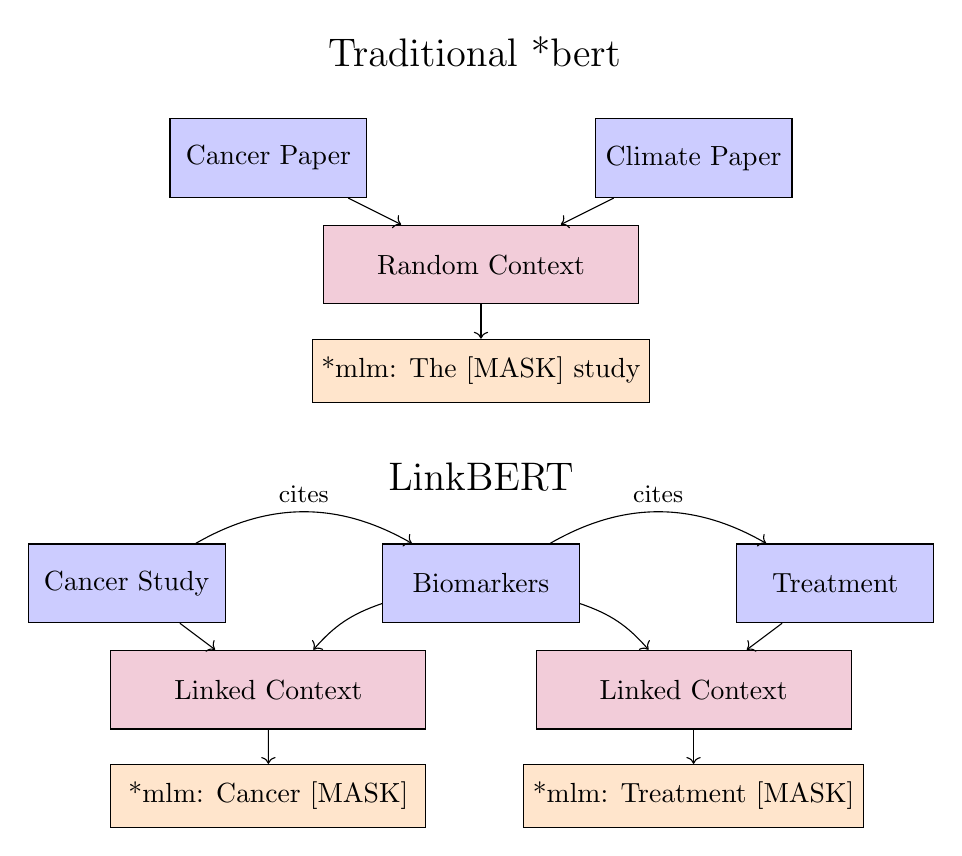
\begin{tikzpicture}[
        doc/.style={rectangle, draw, fill=blue!20, minimum width=2.5cm, minimum height=1cm},
        window/.style={rectangle, draw, fill=purple!20, minimum width=4cm, minimum height=1cm},
        mlm/.style={rectangle, draw, fill=orange!20, minimum width=4cm, minimum height=0.8cm},
        node distance=2cm,
        scale=0.9
    ]
    % Traditional BERT (top)
    \node[align=center] at (-3,5) {\Large Traditional \gls*{bert} };
    \node[doc] (a1) at (-6,3.5) {Cancer Paper};
    \node[doc] (a2) at (0,3.5) {Climate Paper};
    \node[window] (b1) at (-3,2) {Random Context};
    \node[mlm] (m1) at (-3,0.5) {\gls*{mlm}: The [MASK] study};
    
    \draw[->] (a1) -- (b1);
    \draw[->] (a2) -- (b1);
    \draw[->] (b1) -- (m1);
    
    % LinkBERT (bottom) - with increased horizontal spacing
    \node[align=center] at (-3,-1) {\Large LinkBERT};
    \node[doc] (c1) at (-8,-2.5) {Cancer Study};
    \node[doc] (c2) at (-3,-2.5) {Biomarkers};
    \node[doc] (c3) at (2,-2.5) {Treatment};
    
    \node[window] (d1) at (-6,-4) {Linked Context};
    \node[mlm] (n1) at (-6,-5.5) {\gls*{mlm}: Cancer [MASK]};
    
    \node[window] (d2) at (0,-4) {Linked Context};
    \node[mlm] (n2) at (0,-5.5) {\gls*{mlm}: Treatment [MASK]};
    
    % Citations with curved arrows
    \draw[->, bend angle=30] (c1) to[bend left] node[midway,above] {\small cites} (c2);
    \draw[->, bend angle=30] (c2) to[bend left] node[midway,above] {\small cites} (c3);
    
    % Context connections with slight bends to avoid overlap
    \draw[->] (c1) -- (d1);
    \draw[->] (c2) to[bend right=15] (d1);
    \draw[->] (c2) to[bend left=15] (d2);
    \draw[->] (c3) -- (d2);
    \draw[->] (d1) -- (n1);
    \draw[->] (d2) -- (n2);
    
    \end{tikzpicture}
    \caption{Comparison of document processing in traditional \gls*{bert} versus LinkBERT. Traditional \gls*{bert} (top) randomly groups documents into context windows, while LinkBERT (bottom) uses citation relationships to create meaningful document groupings for pretraining. The citation-based grouping ensures that semantically related documents are processed together during \gls*{mlm} tasks.}
    \label{fig:linkbert-comparison}
\end{figure}

Sparse encoder approaches like SPLADE for \gls*{cal} have recently been explored outside the medical domain. It leverages a \gls*{mlm} head to expand each token in a document based on contextual cues from the surrounding text. Rather than extracting a single [CLS] embedding, SPLADE predicts a full vocabulary distribution for each token and aggregates these token-level distributions (via max pooling and sparsity regularisation) to form a sparse document representation. This technique preserves many advantages of bag-of-words approaches (e.g., interpretability, efficiency) while injecting knowledge gleaned from large-scale language model pre-training.

Yang et al. found that replacing TF–IDF or BM25 features with SPLADE-based sparse vectors yields a 10–20\% cost reduction \cite{yang_contextualization_2024}. Crucially, these gains arise because the model can capture synonyms, paraphrases, or other subtle relationships that purely lexical methods miss—accelerating the discovery of relevant studies. This highlights how richer, context-aware document representations enhance the effectiveness of \gls*{cal}, especially under the demanding requirement of near-total recall. The efficacy of medical pre-trained models using SPLADE on medical \gls*{tar} datasets has not been explored.

Research most closely aligned with the central motivation is presented in SciMine \cite{guo_scimine_2023}. This work addresses screening prioritisation within an active learning framework by leveraging inter-document relationships derived solely from the title and abstract. SciMine employs document-level representations generated by SPECTER—a pre-trained transformer model originally developed on citation networks—and enhances these with phrase-level features. The phrase-level module extracts key phrases using a mining tool and obtains contextual embeddings (e.g., via SciBERT), which are subsequently clustered to capture semantic nuances. The approach performs superior to other methods, notably improving early recall and work-saved metrics. However, the technique remains limited in scope as it focuses exclusively on textual and indirect citation-based semantics without fusing additional metadata (such as authorship, publication venue, etc.) that could further improve screening prioritisation.

% https://arxiv.org/pdf/2407.00635 - dense retrieval - is query based

\paragraph{Decoder-based approaches:}
Decoder-based approaches, such as \gls*{llm}+\gls*{cal}, have been outlined and included in this literature review for completeness, as decoder-based work is highly topical. In the typical decoder-based approach, a prompt (with or without explanatory examples) is sent to a model, which generates text/tokens in response. Where \gls*{bert} encodes a passage as a hidden representation, \gls*{gpt}-based models generate text from a unidirectional context.

Decoder-based \gls*{cal} approaches used prompt engineering with a chain-of-thought approach. Bron et al. proposed a novel method, \gls*{llm}+\gls*{cal}, that leverages the capabilities of a decoder-based \gls*{llm} to enhance the screening process in systematic literature reviews~\cite{bron_combining_2024}. This contrasts significantly with the encoder-based methods discussed previously, which primarily focus on generating contextualised representations for ranking. Bron et al.'s approach focuses on developing more fine-grained and explainable classifications by prompting the \gls*{llm} to evaluate each document against individual inclusion criteria specified in the review protocol. Instead of a single binary inclusion/exclusion decision, the \gls*{llm} provides a structured response with reasoning and cited evidence (rationales) for each criterion. This study was, however, only run on a single dataset (Post-traumatic stress disorder systematic review), and the generalisability of this approach is yet established. This criterion-level classification is a unique aspect of their work. It offers potential advantages in integrating \gls*{llm}s to generate 'synthetic' metadata about a document, which can be combined with a document representation. While this approach demonstrates the power of \gls*{llm}s, they still largely focus on individual documents.

Work on prompt selection in decoder-based approaches has demonstrated that active learning can be used to select better representative examples for shot prompting.  Baseline, zero-shot prompting not in an active learning process showed good results on a medical dataset, comparable to decoder BioBERT approaches~\cite{wang_zero-shot_2024}. Few-shot prompting also resulted in better performance \cite{margatina_importance_2022} in combination with active learning. It showed that using active learning to identify and choose the most representative examples significantly improved few-shot prompt performance on downstream tasks. This suggests that strategically combining active learning with prompt engineering could enhance the effectiveness of decoder-based models in \gls*{tar}, even with limited labelled data. While this approach demonstrates the power of \gls*{llm}s, they still largely focus on individual documents, analysing them against inclusion criteria. Even active learning for prompt selection, while improving inter-document representation for prompting, does not yet address the crucial need to model inter-document relationships.  This suggests that while decoder-based methods hold promise, further research is needed to explicitly incorporate relational information into their frameworks. 

While decoder-based approaches might produce rationales or explanations, their ability to handle large-corpus level inter-document relationships is limited by their context window size, which restricts the number of documents and relationships they can represent in a single context.

\subsection{Conclusion}
The reviewed literature consistently demonstrates the benefit of moving beyond shallow text representations. However, even the most advanced encoder- and decoder-based methods do not explicitly utilise the rich inter-document relationships present in medical research.  Incorporating these relationships is crucial for improving \*{cal} in systematic reviews. Tools, such as citation mining and \gls*{gnn}, offer a natural way to represent and reason about these relationships, making them a promising avenue for future research.

\section{Metadata and citation networks}\label{sec:metadata}

% As outlined in the preceding sections, this PhD research aims to enhance the efficiency and accuracy of systematic review screening through \gls*{cal}. 

A key limitation of current \gls*{cal} approaches is their shallow document representation, often neglecting valuable metadata and inter-document relationships within citation networks. This section explores how incorporating these elements can significantly improve document screening prioritisation, addressing the PhD's core objective of minimising expert screening effort while maintaining high recall. Firstly, traditional methods like \gls*{bcs} and \gls*{fcs} are considered. Secondly, \glspl*{gnn} are assessed. Finally, the potential of integrating \glspl*{llm} into the screening process is reviewed.

In scientific research, understanding relationships between documents is critical for identifying relevant literature, tracing ideas' evolution, and assessing individual studies' impact. To situate their findings within the broader literature, authors must reference prior works in their research papers, substantiating claims and demonstrating connections to existing knowledge. This practice relies on standardised formatting conventions and peer-reviewed publication systems, which ensure consistency and credibility in research communication \cite{noauthor_bmc_nodate}. These references form an explicit and analysable indicator of document relationships: the citation network. Specifically, citations documented in a paper's reference section create a structured graph that maps connections between studies. By analysing this network, researchers can infer relationships between papers, assuming that cited or cited works share meaningful relevance to the original research. This signal can be exploited for screening prioritisation as if a researcher has published relevant work towards a search; their other work is likely to be related.

\subsection{Citation network mining}

Performant, simple, and robust citation network mining approaches exist in medical research, i.e., \gls*{bcs} and \gls*{fcs}. The two methods can be understood using the graph network approach outlined below.

\begin{tcolorbox}[title=Citation Network Definitions] 
\small
Let $G = (D, E)$ be a directed citation graph, where each vertex $D_i \in D$ represents a research article, and a directed edge ($D_i, D_j) \in E$ means that $D_i$ cites $D_j$. $D$ represents the universe of all documents in $G$. Let $D_i \in D$ be a document of interest. 

\begin{itemize}
    \item $D_{ip} = {D_j \in D | (D_i, D_j) \in E}$ as the set of articles referenced by $D_i$ (i.e., articles $D_i$ cites). 
    \item $D_{if} = {D_j \in D | (D_j, D_i) \in E}$ as the set of articles that reference $D_i$ (i.e, articles that cite $D_i$).

\end{itemize}

In most citation graphs (which are usually directed acyclic graphs, or at least lack reciprocal citations), the set of articles cited by a given paper and the set of articles that cite it are disjoint: $D_{ip} \cap D_{if} = \emptyset$. This is because a single edge represents only a citation relationship in a temporal direction. Searching both sets will, therefore, provide different relevant articles.
\newline
\newline
Two primary citation network mining approaches are defined, utilising the sets of related articles:

\begin{itemize}
    \item \gls*{bcs}:  This approach examines the set of articles \emph{cited by} the paper of interest, $D_{ip}$.  In practice, this involves analysing the relevancy of each article in $D_{ip}$ to the research question. \cite{lefebvre_cochrane_2011, akers2009systematic}
    \item \gls*{fcs}: This approach examines the set of articles that \emph{cite} the paper of interest, $D_{if}$.  Similarly, the relevancy of each article in $D_{if}$ is assessed\footnote{\gls*{fcs} involves using a citation index to identify studies that cite a source study. A citation index is a database of scholarly articles and their citations, such as PubMed, Google Scholar, Scopus or OpenAlex.}.
\end{itemize}

\end{tcolorbox}


% Research on using BCS and FCS in screening:
\gls*{bcs} and\gls*{fcs} are valuable tools within the identification phase of systematic reviews, helping researchers discover relevant studies by leveraging citation relationships to form the total document pool. They are not yet, however, utilised within the screening process that this research will focus on (as traditional approaches look at all documents within the pool). Even the use of \gls*{bcs} in the \emph{identification phase} (as mandated by the Cochrane Handbook, criterion C30~\cite{noauthor_mecir_nodate}) is not ubiquitous, with 87\% of sampled systematic reviews reportedly using \gls*{bcs} and 9\% \gls*{fcs} \cite{briscoe_conduct_2019}. Within this context, success is often measured by the number of relevant articles retrieved, with studies demonstrating the benefits of \gls*{bcs}/\gls*{fcs} in increasing recall. For example, research consistently shows that utilising \gls*{bcs} and \gls*{fcs} improves the retrieval of eligible articles, with the vast majority of studies (over 96\%) reporting some level of benefit \cite{hirt_citation_2023}. This research highlights the important role these methods play in comprehensive literature searching, yet they are not utilised within \gls*{cal}, which effectively searches for relevant documents for humans to screen. A search of relevant literature (see Figure \ref{fig:search-results}) demonstrates that neither \gls*{bcs} nor \gls*{fcs} has been integrated into \gls*{cal} processes.

\begin{figure}[t]
\begin{center}
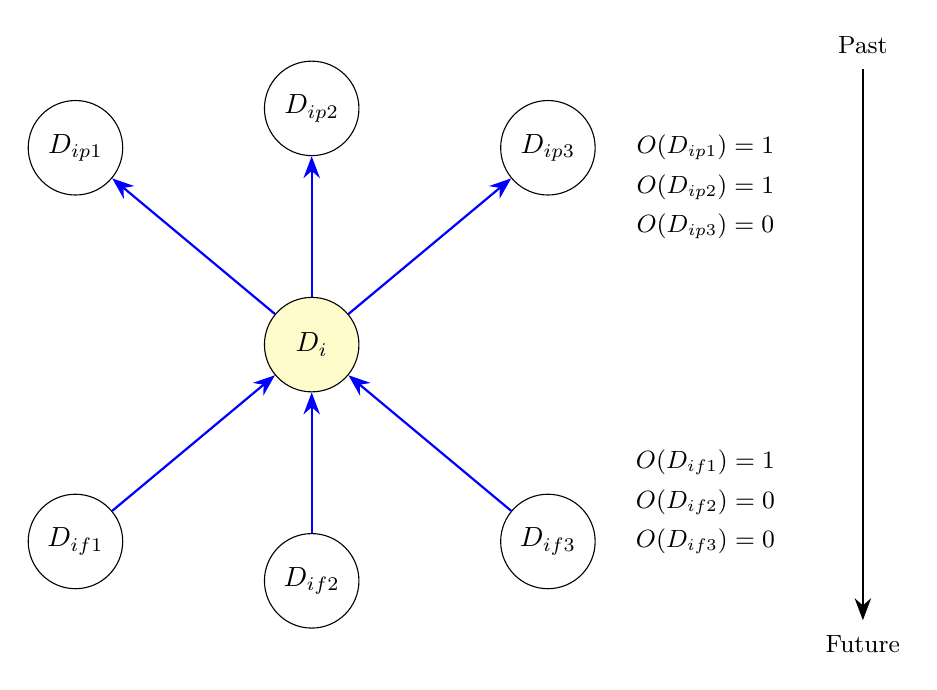
\begin{tikzpicture}[
    >={Stealth[scale=1.2]}, % Use a standard arrow tip like Stealth
    vertex/.style = {circle, draw, minimum size=1.2cm, inner sep=1pt},
    ref_edge/.style = {->, thick, blue},
    label_style/.style = {font=\small}
]
% Main document Di
\node[vertex, fill=yellow!20] (Di) at (0,0) {$D_i$};

% Past references (Dip) - More fanned out
\node[vertex] (Dip1) at (-3,2.5) {$D_{ip1}$};
\node[vertex] (Dip2) at (0,3) {$D_{ip2}$};
\node[vertex] (Dip3) at (3,2.5) {$D_{ip3}$};

% Future references (Dif) - More fanned out
\node[vertex] (Dif1) at (-3,-2.5) {$D_{if1}$};
\node[vertex] (Dif2) at (0,-3) {$D_{if2}$};
\node[vertex] (Dif3) at (3,-2.5) {$D_{if3}$};

% Edges for past references
\draw[ref_edge] (Di) -- (Dip1);
\draw[ref_edge] (Di) -- (Dip2);
\draw[ref_edge] (Di) -- (Dip3);

% Edges for future references
\draw[ref_edge] (Dif1) -- (Di);
\draw[ref_edge] (Dif2) -- (Di);
\draw[ref_edge] (Dif3) -- (Di);

% Labels for sets
% \node[label_style] at (-4,2) {$D_{ip}$ (Referenced by $D_i$)};
% \node[label_style] at (-4,-2) {$D_{if}$ (References to $D_i$)};

% Relevancy function examples
\node[label_style] at (5,2.5) {$O(D_{ip1}) = 1$};
\node[label_style] at (5,2) {$O(D_{ip2}) = 1$};
\node[label_style] at (5,1.5) {$O(D_{ip3}) = 0$};
\node[label_style] at (5,-1.5) {$O(D_{if1}) = 1$};
\node[label_style] at (5,-2) {$O(D_{if2}) = 0$};
\node[label_style] at (5,-2.5) {$O(D_{if3}) = 0$};

% Time arrow (vertical)
\draw[->, thick] (7,3.5) -- (7,-3.5); % Stealth is already set as default
\node[label_style] at (7,3.8) {Past};
\node[label_style] at (7,-3.8) {Future};

\end{tikzpicture}
\label{fig:bcs-fcs-explained}
\caption{Visual comparison of \gls*{bcs} and \gls*{fcs} approaches. Note that citation mining effectively operates on a temporal axis.}
\end{center}
\end{figure}

% How this approach will benefit CAL
The logical and simple augmentation of the encoder \gls*{cal} approach would be to exhaust both the \gls*{bcs} and \gls*{fcs} networks of a seed document before initiating the encoder \gls*{cal} process. A simple and performant approach could be achieved by first identifying all documents related to the seed document through \gls*{bcs} or \gls*{fcs} searches, assessing their relevance, and then adding the labelled documents to the training data used in the first epoch of the encoder \gls*{cal} process (see Figure 2.6). The theoretical benefits of citation network mining are that it can be used to augment the \gls*{cal} process in ways that overcome some of the limitations of this process. Firstly, \gls*{cal} requires labelled data to train a classifier model, which is assumed to perform better with more data points. Encoder \gls*{cal} approaches suffer disproportionately from feature-based \gls*{cal} approaches due to their need for larger training data to effectively learn meaningful representations, as they need to learn complex contextual relationships between words and concepts. Feature-based models, in contrast, can rely on simpler statistical patterns. When working with limited labelled data in the early screening stages, encoder models may struggle to generalise well, potentially leading to suboptimal performance in identifying relevant documents. Citation mining can also neatly fit into the existing performant encoder \gls*{cal} process, as a single sample seed document is often used during the first epoch for fine-tuning. A better approach would be to exhaust the \gls*{bcs}/\gls*{fcs} citation network of that seed document for labelling before using revealed relevant documents to fine-tune the model, potentially resulting in a more performant model at the earlier screening stages with less Oracle cost.

While \gls*{bcs} and \gls*{fcs} are effective methods for initial document discovery, they are inherently limited by their reliance on direct citation links. This reliance prevents them from identifying thematic connections between uncited yet related documents. This limitation is particularly relevant because the initial document pool is vastly smaller than the total scholarly literature, increasing the likelihood of important non-direct citations. Furthermore, \gls*{bcs} and \gls*{fcs} do not consider the semantic content of the papers beyond the presence or absence of citation links. This potential citation disconnection could mean relevant documents that do not share direct citations or use different terminology to describe similar concepts may be missed. Additionally, constraining document representations to the title, abstract, and citation analysis miss other relevant features, such as author information, publication date, or journal. Previous work by this author has demonstrated that additional features are important for downstream document classification tasks - see Appendix \ref{app:Predicting_article_retractions}. Publication year was found to be the most important feature when using standard feature-based and encoder- and decoder-based \glspl*{llm} (more so than the title and abstract). It might be argued that the importance of this feature might be specific to that task (i.e., retraction classification); yet, logically, it follows that when searching through a pool of documents, publication year could be an important signal for relevance, as knowledge of that search area improves, so does the definition, experimental design and even disease classification process improves.

These limitations highlight the need for a more sophisticated approach to capturing the full complexity of structural and semantic inter-document relationships. \glspl*{gnn} excel precisely in this area: They can capture multi-hop relationships (e.g., documents that share a chain of citations), leverage co-author networks, or incorporate publication venues.

\subsection{Advanced graph approaches}

\glspl*{gnn} can model the citation network in a way that goes beyond direct citation links, allowing for identifying relevant documents based on structural and semantic similarity. By incorporating document metadata and leveraging advanced techniques like message passing, \glspl*{gnn} can capture complex relationships that are not apparent when using \gls*{bcs}/\gls*{fcs} alone. This approach allows us to represent documents not only by their textual content (title and abstract) but also by their \gls*{bcs} or \gls*{fcs} links and associated metadata. \glspl*{gnn} are a family of deep learning models specifically designed to analyse data structured as graphs \cite{lee_attention_2018, wu_comprehensive_2021, bronstein_geometric_2017, khemani_review_2024}. Unlike traditional neural networks, such as \glspl*{cnn} and Recurrent Neural Networks, which excel at processing grid-like or sequential data, respectively, \glspl*{gnn} are adept at leveraging the inherent relationships within graph data. These relationships can be represented as nodes (documents) and edges (connections) – see Figure \ref{fig:GNNs}. \glspl*{gnn} find applications in diverse areas, such as modelling interactions between users and products in e-commerce for recommendation systems or categorising research papers within citation networks. 

The fundamental mechanism behind \glspl*{gnn} is ``message passing". This iterative process involves each node aggregating information from its neighbouring nodes and subsequently updating its own representation based on this aggregated data. Message passing allows \glspl*{gnn} to capture complex dependencies and patterns that are not easily discernible in traditional Euclidean space. This process can be thought of as passing ``relevance signals" through the \glspl*{gnn}, potentially allowing early identification of relevant clusters, enabling faster stopping and, thus, less screening.

Within the broader \gls*{gnn} landscape, various architectures exist, each employing a unique approach to message passing. A \gls*{gcn} \cite{berg_graph_2017} utilises a form of weighted averaging, combining the feature vectors of neighbouring nodes with weights derived from the graph structure. They then apply transformations to these combined features. gls*{gcn}s have demonstrated success in applications such as recommendation systems \cite{fan_graph_2019}, image classification \cite{monti_geometric_2016}, and traffic forecasting \cite{cui_traffic_2020}. \glspl*{gat} enhance this process by incorporating an attention mechanism. This mechanism dynamically weighs the importance of each neighbour's features during aggregation, allowing the model to focus on the most relevant connections. GraphSAGE offers a different approach, focusing on inductive representation learning. It learns aggregation functions that sample and combine features from a node's neighbourhood, enabling generalisation to unseen nodes. 

While a comprehensive exploration of each \gls*{gnn} variant is beyond the scope of this review, it is important to note that these architectures show significant promise for document classification due to their ability to model complex relationships between documents. The next section considers how \glspl*{gnn} can be integrated into the document classification.
\begin{figure}[h!]
    \centering
    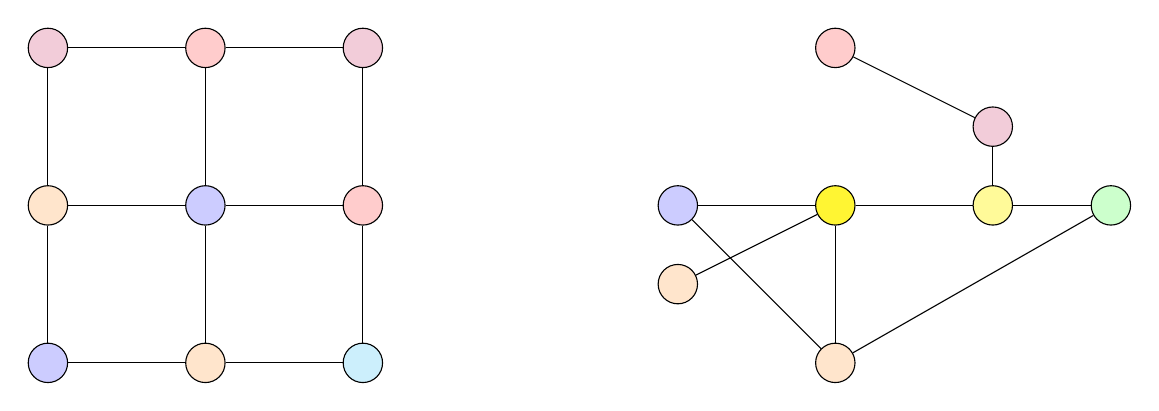
\begin{tikzpicture}
        % Euclidean Space (Left)
        \begin{scope}
            \node[circle, fill=blue!20, draw, minimum size=0.5cm] (A) at (0,0) {};
            \node[circle, fill=orange!20, draw, minimum size=0.5cm] (B) at (2,0) {};
            \node[circle, fill=cyan!20, draw, minimum size=0.5cm] (C) at (4,0) {};
            \node[circle, fill=orange!20, draw, minimum size=0.5cm] (D) at (0,2) {};
            \node[circle, fill=blue!20, draw, minimum size=0.5cm] (E) at (2,2) {};
            \node[circle, fill=red!20, draw, minimum size=0.5cm] (F) at (4,2) {};
            \node[circle, fill=purple!20, draw, minimum size=0.5cm] (G) at (0,4) {};
            \node[circle, fill=red!20, draw, minimum size=0.5cm] (H) at (2,4) {};
            \node[circle, fill=purple!20, draw, minimum size=0.5cm] (I) at (4,4) {};

            \draw (A) -- (B);
            \draw (B) -- (C);
            \draw (D) -- (E);
            \draw (E) -- (F);
            \draw (G) -- (H);
            \draw (H) -- (I);
            \draw (A) -- (D);
            \draw (B) -- (E);
            \draw (C) -- (F);
            \draw (D) -- (G);
            \draw (E) -- (H);
            \draw (F) -- (I);
        \end{scope}
        
        % GNN In Euclidean Space (Right)
        \begin{scope}[xshift=8cm]
            \node[circle, fill=blue!20, draw, minimum size=0.5cm] (A) at (0,2) {};
            \node[circle, fill=orange!20, draw, minimum size=0.5cm] (B) at (2,0) {};
            \node[circle, fill=yellow!80, draw, minimum size=0.5cm] (C) at (2,2) {};
            \node[circle, fill=yellow!40, draw, minimum size=0.5cm] (D) at (4,2) {};
            \node[circle, fill=purple!20, draw, minimum size=0.5cm] (E) at (4,3) {};
            \node[circle, fill=red!20, draw, minimum size=0.5cm] (F) at (2,4) {};
            \node[circle, fill=green!20, draw, minimum size=0.5cm] (G) at (5.5,2) {};
            \node[circle, fill=orange!20, draw, minimum size=0.5cm] (H) at (0,1) {};

            \draw (A) -- (B);
            \draw (A) -- (C);
            \draw (B) -- (C);
            \draw (C) -- (D);
            \draw (C) -- (H);
            \draw (D) -- (E);
            \draw (D) -- (G);
            \draw (E) -- (F);
            \draw (G) -- (B);
        \end{scope}
    \end{tikzpicture}
    \caption{Grid Graph (Euclidean Structure) (Left), Arbitrary Graph (Non-Euclidean Structure) (Right)}
    \label{fig:GNNs}
\end{figure}

\begin{tcolorbox}[title=Conceptualising the integrating \glspl*{gnn} for document classification]  
\small


  A node is represented by a feature matrix containing information about the document. This \textbf{Node feature matrix}, $X$, which has the dimensions of $m$ (the number of nodes) and $n$ (the number of features). $X \in \mathbb{R}^{m \times n}$. X does not have to be a square matrix and does not encode any information about the graph's structure. 

  Consider three research papers as nodes, with features: [Author, Title Length, Abstract Length, Citation Count]
  $X = \begin{bmatrix}
  \text{"Smith"} & 82 & 500 & 45 \\
  \text{"Johnson"} & 95 & 475 & 23 \\
  \text{"Zhang"} & 67 & 612 & 89
  \end{bmatrix}$
  Where $X \in \mathbb{R}^{3 \times 4}$ represents:
  
  3 papers (rows)
  4 features per paper (columns)
  Mixed data types (categorical and numerical)

  Structural information is encoded in the \textbf{adjacency matrix}, $A$, which has the dimensions of $m$ (the number of nodes) and $m$ (the number of nodes). $A \in \mathbb{R}^{m \times m}$. A encodes information about the graph's structure and is used to determine relationships between nodes. Conventionally, the source nodes are the rows, and the destination nodes are the columns of the matrix. 1 indicates an edge between the source node $u$ and destination node $v$. Note that there is a choice here, with the matrix diagonal being 0 or 1. This choice is based on whether you consider the source node connected to itself. In cases where the representation of the node depends on itself and adjacent nodes, the diagonal should be set to 1. In the scenario of citation networks, the diagonal should be set to 1, as a paper is likely to reference and build upon its own findings throughout. Setting the diagonal to 0 is akin to attempting to predict the representation of the node based only on its adjacent nodes, which is not the case in citation networks. If an adjacency matrix is symmetric around it's diagonal, then the graph is undirected, otherwise it is directed (i.e. $U$ is connected to $V$ and $V$ is connected to $U$). In citation networks, this is not the case, as because paper A cites paper B, it does not mean the reverse is true.    

  Consider the same three research papers with the following adjacency matrix:
  $A = \begin{bmatrix}
  0 & 1 & 0 \\
  0 & 0 & 1 \\
  1 & 0 & 0
  \end{bmatrix}$
  Which represents the following graph:

  \begin{center}
    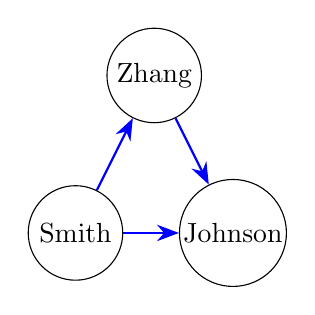
\begin{tikzpicture}[
        > = {Stealth[scale=1.2]},
        vertex/.style = {circle, draw, minimum size=1.2cm, inner sep=1pt},
        ref_edge/.style = {->, thick, blue},
        label_style/.style = {font=\small}
    ]

    \node[vertex] (Smith) at (0,0) {Smith};
    \node[vertex] (Johnson) at (2,0) {Johnson};
    \node[vertex] (Zhang) at (1,2) {Zhang};

    \draw[ref_edge] (Smith) -- (Johnson);
    \draw[ref_edge] (Zhang) -- (Johnson);
    \draw[ref_edge] (Smith) -- (Zhang);
    \end{tikzpicture}
    \end{center}

    With both $X$ and $A$ defined, we can numerically represent the graph. The node feature matrix $X$ is the initial/input node features, with our goal for learning on graphs to learn node embeddings $H \in \mathbb{R}^{N\times D}$ where $D$ is a chosen hidden dimension size. 


   
\end{tcolorbox}

\begin{tcolorbox}[title=Message Passing Neural Networks in \glspl*{gnn}]  
\small
    \glspl*{cnn}, designed for grid-structured data like images, rely on fixed-size convolutional filters to learn spatial invariance. However, graphs present a challenge. Their variable size and non-grid structure mean these filters, effective for image grids, are not directly applicable. Therefore, Message Passing Neural Networks (MPNNs) were developed. MPNNs address this limitation by using message passing, a graph-native approach, to learn representations from the irregular structure of graphs, effectively achieving a form of spatial (or rather, structural) invariance suitable for graph data.

    The process is defined as follows:
    \begin{itemize}
        \item {\bf{Message:}} every node decides how to send information to neighbouring nodes it is connected to by edges
        \item {\bf{Aggregate:}} nodes receive messages from all their neighbours, who also pass messages and decide how to combine the information from all of their neighbours. 
        \item {\bf{Update:}} each node decides how to combine neighbourhood information with its own information and updates its embedding for the next time step. 
    \end{itemize}

    By doing this, nodes pass each other information and disseminate information around the graph, allowing the network to learn spatial invariance.  This can be repeated for a fixed number of iterations ($k$), with the larger the value of $k$, the more the more diffuse the information around the graph becomes.

    The message passing process can be further clarified:

    \begin{itemize}
        \item {\bf{Message:}} The source node $U$ will pass a message $m_{uv}$ to the destination node $V$. The message depends on the \gls*{gnn} architecture, with the easiest example message being passed being $U$ node's feature $h_u$ vector to $V$.
        \item {\bf{Aggregate: }} The destination node $V$ will receive messages from all its neighbouring nodes and needs to decide how to combine the information from all of its neighbours. This is typically done using a sum, average or max pooling of the messages from all neighbouring nodes. It is important that the aggregation function has to be a permutation invariant function, as the order of the messages should not affect the output. This gives us a combined neighbourhood node embedding, denoted as $h_{N(V)}$, where $N(V)$ is the set of all neighbouring nodes to $V$, meaning all nodes connected to $V$ by an edge. $h_{N(v)}^{k+1} = AGGREGATE({h_u^k, \forall u \in N(v)})$
        \item {\bf{Update: }} Each node updates its own embedding based on the combined neighbourhood embedding and its own embedding from the previous timestep. $h_v^{k+1} = \sigma(W \cdot CONCAT(h_v^k, h_{N(v)}^{k+1}))$
    \end{itemize}

\end{tcolorbox}

\subsection{Graph neural networks for document classification}

Modelling document relationships as citations allows us to leverage a homogeneous graph structure. Each node represents a research paper, and edges depict relationships between these papers, such as citations or co-authorship. This structure results in a uniform type for both nodes and edges.

\glspl*{gnn} offer two primary learning paradigms for node prediction: transductive and inductive learning. Transductive learning leverages the entire graph structure during training to infer labels for unlabelled nodes within that same graph. Conversely, inductive learning trains on a subset of the graph, enabling it to generalise and predict labels for previously unseen documents. Transductive \glspl*{gnn} can be particularly useful for systematic review screening because they leverage the relationships between documents within a fixed set to enhance the screening process. Similarly, inductive \gls*{gnn}s facilitate automated screening of new papers, improving efficiency and scalability and providing a strategy to integrate these new documents into the graph, potentially lending themselves more to a systematic review update. Given the temporal nature of research publications, where papers cannot cite each other bidirectionally, a directed (i.e., edges explicitly flow from one node to another) graph models these relationships appropriately. Furthermore, since the larger pool of documents remains constant during the screening phase, the graph is static (i.e., not evolving).


\paragraph{\gls*{gnn} document representation approaches:}
Researchers have achieved \gls*{gnn} document representation via different approaches. For example, Yao et al. proposed a transductive approach called Text \gls*{gcn} \cite{yao_graph_2018}, which constructs a single, global graph representing the entire corpus. In this global graph, nodes represent both words and documents, and edges reflect word co-occurrence across the corpus and document-word relationships using methods like \gls*{tfidf}. While this approach effectively captures global word co-occurrence, it struggles with unseen documents and prioritises corpus-level relationships over document-level contextual nuances. Later, Zhang et al. built individual graphs for each document and then used a GNN to learn the fine-grained word representations based on their logical structures \cite{zhang_evaluating_2020}. They construct these graphs using a sliding window inside each document, allowing them to capture contextual word relationships. Creating individual graphs for each document also enables inductive learning of new words, overcoming another limitation of previous approaches. GNN document representation was advanced further with the conTextING approach by combining the per-document graph with \glspl*{bert}  contextual embeddings \cite{huang_contexting_2022}. More recently, Piao et al. proposed a novel method called Sparse Structure Learning \cite{piao_sparse_2022}, which builds upon these prior works by creating trainable, individual, and sparse graphs for each document. This method starts with sentence-level subgraphs and then learns to connect them sparsely, capturing both local syntactic and global semantic information while dynamically adjusting to the specific structure of each document. These four papers highlight a progression in \gls*{gnn}-based text classification: from leveraging global, corpus-wide information via a single, large graph (Text \gls*{gcn}) to focusing on local, document-specific information through individual graphs and inductive learning (TextING/conTextING) and finally to learning dynamic, sparse graph structures tailored to each document (Sparse Structure Learning). However, these approaches primarily focus on textual features. This research, in contrast, will investigate integrating structural features (citations) and document metadata to enhance \gls*{gnn}-based document classification further.

\paragraph{Node Classification in \glspl*{gnn}:}
\glspl*{gnn} can operate at the node level to classify documents \cite{kipf_semi-supervised_2017, yao_graph_2018, wang_graph_2024, rong_dropedge_2020}. This means they can classify individual documents (nodes) based on their content and connections within the graph, potentially enhancing document representation and information integration. Node-level classification is particularly relevant when dealing with unlabelled data, which aligns with the active learning premise of this PhD.

% leveraging citation and metadata
Research specifically on document classification using \glspl*{gnn} demonstrates their performance. Ly et al. classified research output into context-specific categories by enriching a simple \gls*{gnn} with representations that encode references, co-authorships, shared publication sources, and subject headings as distinct edge types \cite{ly_article_2024}. They demonstrated that using multi-graphs (i.e. more than one edge allowed between nodes, each denoting a different type of relationship) to encode this data consistently improved the performance of various \gls*{gnn} models on a PubMed diabetes dataset. Zhang et al.'s work used on medical bibliographic classification task demonstrated increased performance when utilising a novel Transformer-based heterogeneous \gls*{gnn}, namely Text Graph Transformer (TG-Transformer), which captures structure and heterogeneity from the text graph and is scalable to large-sized corpora due to a mini-batch text graph sampling method \cite{zhang_evaluating_2020}. This method significantly reduces computing and memory costs, making TG-Transformer outperform state-of-the-art approaches on text classification tasks. The authors also found that modelling heterogeneity information and including structural encodings and pre-trained word embeddings further improved performance.

All this research supports the premise that representing a document less shallowly (i.e., with a \gls*{gnn} architecture) results in improved classification performance. Better representation is not an end in itself but a means to reduce screening loads and ensure near-total recall in a fraction of the time.

\paragraph{Active learning with \glspl*{gnn}:}
Work on using \gls*{gnn} node classification in an active learning setting has been reviewed \cite{madhawa_active_2020}. Katsimpras proposed a framework that first uses active learning to select highly uncertain unlabelled nodes to be labelled and included in the training dataset \cite{katsimpras_improving_2024}. While their approach is not exactly a \gls*{cal} approach (they created pseudo labels to augment training with \emph{uncertain} data points), it demonstrates that active learning can be used. Building upon this, the recent FICOM (Feature Influence Diversified COverage Maximization) paper by Zhang et al. introduces a novel active learning framework specifically designed for \glspl*{gnn} in semi-supervised node classification tasks \cite{zhang_ficom_2024}. FICOM addresses key challenges in this area, such as scalability to large graphs and the need for effective node selection criteria. The authors proposed a unique approach combining Personalized PageRank coverage to capture node importance in the graph structure with embedding diversity to account for feature similarity. Both of these researchers did not use a \gls*{cal} approach.

Another approach to integrating active learning with \glspl*{gnn} was generating a node representation of a document through a \gls*{gcn}, passing messages, and selecting the most informative nodes for labelling \cite{wu_active_2021}. This representation was then used for k-medoids clustering, with a cluster's label centre being queried. This allows for choosing the most representative nodes within a cluster, reflecting the diversity of the document collection. The intuition behind this method is that nodes closest to the cluster centre are likely to be more informative and contribute significantly to the learning process of the \gls*{gnn}. By selecting these central nodes, less annotation cost was achieved for better performance. This research did not use a \gls*{cal} approach (as it set $k$ for message passing to the budget), so it did not align strongly with the systematic review process. This research shows two things: 1) document representations through a \gls*{gnn} architecture can be performant, and 2) \gls*{gnn} use in active learning shows potential for reducing annotation cost.

\paragraph{Prompt engineering:}
\glspl*{llm} can be strategically integrated as enhancers within this framework to enrich document representations further and enhance the capabilities of \glspl*{gnn}. As outlined, citation network graph analysis occurs above the document level by utilising extracted features about documents. \glspl*{llm} are a natural replacement for feature extraction, as they possess the increased ability to understand the semantic meaning of documents. The ultimate goal of using \gls*{llm}s and graph networks is to complement and enhance issues with each other. 

Research has been conducted into using \glspl*{llm} within the \glspl*{gnn} and has developed a robust taxonomy for categorising \gls*{llm}s~\cite{ren_survey_2024}. A promising application of \glspl*{llm} within graph networks is to use \gls*{llm} as an enhancer. \glspl*{llm} can encode text into nodes using more complex features, such as semantic meaning, which can be used within the \glspl*{gnn}~\cite{zolnai-lucas_stage_2024}.
    
Explanation-based enhancers query an \gls*{llm} using prompting to capture higher-level features about documents, which is used to enrich node representations before processing with a \gls*{gnn}, with the process being abstracted in Figure \ref{fig:llm4g}. He et al. used the approach that prompted \gls*{gpt} 3.5 with a document's abstract and text and questions about that document using a zero-shot approach~\cite{he_harnessing_2024}. The \gls*{llm} response then forms features that are amended to the original node representations. This approach requires domain-specific knowledge, as features deemed important (and hence prompt used) depend on the research domain. It was performant in the PubMed domain, scoring greater node classification accuracy using this approach. These results suggest that \gls*{llm}-based feature enrichment can significantly improve the performance of \glspl*{gnn} on document classification tasks.

\begin{figure}[h]
    \centering
    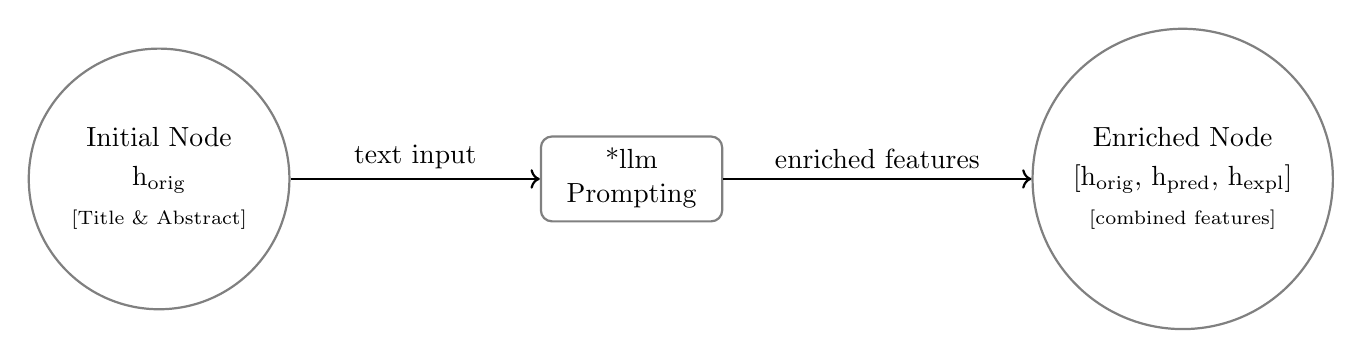
\begin{tikzpicture}[node distance=3cm,auto]
        
        % Define styles
    \tikzstyle{node} = [circle, minimum width=2.5cm, minimum height=2.5cm, draw=black!50, thick]
    \tikzstyle{process} = [rectangle, rounded corners, minimum width=2cm, minimum height=1cm, draw=black!50, thick]
    \tikzstyle{features} = [text width=2cm, align=left]
        
        % Initial node
    \node[node] (initial) {
            \begin{tabular}{c}
                Initial Node\\[2pt]
                h\textsubscript{orig}\\[2pt]
                \scriptsize{[Title \& Abstract]}
            \end{tabular}
        };
        
        % Process box
    \node[process, right of=initial, xshift=3cm] (process) {
            \begin{tabular}{c}
               \gls*{llm} \\Prompting
            \end{tabular}
        };
        
        % Enriched node
    \node[node, right of=process, xshift=4cm] (enriched) {
            \begin{tabular}{c}
                Enriched Node\\[2pt]
                [h\textsubscript{orig}, h\textsubscript{pred}, h\textsubscript{expl}]\\[2pt]
                \scriptsize{[combined features]}
            \end{tabular}
        };
        
        % Arrows
    \draw[->, thick] (initial) -- (process) node[midway, above] {text input};
    \draw[->, thick] (process) -- (enriched) node[midway, above] {enriched features};
        

        
    \end{tikzpicture}
    \caption{Node feature enrichment process using an \gls*{llm}.}
    \label{fig:llm4g}
    \end{figure}

\paragraph{Screening prioritisation with active Learning using \glspl*{gnn}:}
While research explores \glspl*{gnn} in active learning settings, a significant gap in the literature remains: the application of \glspl*{gnn} within a \gls*{cal} framework, specifically designed for the unique demands of systematic review document screening and leveraging the rich information available in metadata and citation networks. This PhD research will directly address this gap. 

\paragraph{Content-Based Recommender Systems for existing systematic reviews:}
Tenti et al. have previously shown that integrating OpenAlex and Microsoft Academic Graph metadata into recommender systems increases precision~\cite{tenti_contreviews_2025}. The \gls*{cbrs} fundamentally differs from the active learning paradigm, as \gls*{cbrs} aims to provide recommendations based on an existing document pool. In contrast, active learning recommends documents iteratively to learn from. Furthermore, Tenti focused on pre-existing systematic reviews, whereas active learning approaches tend to be utilised to generate new systematic reviews. Additionally, while Tenti used metadata to improve the performance of their \gls*{cbrs}, it did not consider document relationships.

\subsection{Conclusion}
A critical shortcoming in current screening approaches for systematic reviews using active learning is their tendency to treat each document as an isolated text. Commonly, only the title and abstract are used to prioritise documents for manual screening, neglecting the rich metadata available in bibliographic databases (e.g., publication year, venue, or author information) and the structures inherent in citation networks. Traditional methods like \gls*{bcs} and \gls*{fcs} help identify relevant studies by tracing references across papers, but they remain limited to direct citations. Consequently, they overlook deeper or indirect relationships—such as shared co‐authors, research topics, or citation ``chains"—that could reveal additional high‐value documents.

\gls*{gnn} models offer a way to exploit these richer inter‐document relationships. \glspl*{gnn} can treat each document as a node enriched with metadata and connected by edges (citations or co‐authorship links), enabling ``message‐passing" that propagates relevance signals across the network. Incorporating metadata and citation information in this way has shown promise for improving accuracy and reducing screening efforts. Although GNN‐based classification has succeeded in analogous tasks, few—if any—published approaches integrate \glspl*{gnn} into a \gls*{cal} workflow specifically for medical systematic reviews. Two methods could be explored: 1) How using \gls*{gnn} document representations (along with metadata) can improve the encoder \gls*{cal} process, and 2) How to utilise a \gls*{gnn} to recommend articles for screening based on a dynamic update of the \glspl*{gnn} understanding of document relevance based on an oracle updating documents within it. 

% The PhD is driven by the need to minimise expert screening time while safeguarding near‐total recall in systematic reviews. Existing \gls*{cal} pipelines already reduce effort relative to manual screening but still rely on shallow document representations. By systematically integrating metadata (e.g., publication date, journal status) and citation networks (e.g., references, co‐authors) into \gls*{cal}, this PhD aims to rank and prioritise relevant documents more intelligently. Doing so could surface key studies earlier—allowing reviewers to find the needed evidence faster.



\section{Stopping algorithms}\label{sec:Stopping_algorithms}

Once a prioritisation strategy effectively ranks potentially relevant studies, knowing when to stop remains essential for reducing screening costs in systematic reviews. Even the best prioritisation scheme is of limited use if the entire pool is screened, so these stopping approaches strive to balance cost against retrieval. In an idealised scenario, if the total number of relevant documents is known ahead of time and used to guide stopping with a target recall of 100\%, system efficiency depends solely on how well documents are ranked. By contrast, setting the target recall below 100\% now allows efficiency to be dictated by the ranking \emph{and} the stopping method. In practice, 100\% recall is not required to answer the search question; therefore, efficiency improvements can come from improving screening prioritisation \emph{and} stopping algorithms. Many systematic review approaches in \gls*{tar} adopt near-total recall thresholds (e.g., 95\%). Traditional approaches to stopping assume the goal is total coverage of relevant items. Yet in reality, humans often stop earlier, guided by factors such as time constraints, perceived sufficiency of information, or intuitive notions of diminishing returns \cite{ilani_analysis_2024, browne_cognitive_2007, wu_online_2014}.

User studies in broader \gls*{ir} contexts confirm that stopping decisions are multifaceted, shaped by both cognitive and environmental factors \cite{ilani_analysis_2024}. Cognitive factors include the searcher’s sense of ``information sufficiency", personal experience, and tolerance for ``bad" or irrelevant information. Environmental factors include the nature of the task (e.g., urgency or complexity), time or resource constraints, and the retrieval system's ability to yield relevant evidence \cite{prabha_what_2007}. Although systematic reviews involve multiple screeners and formal protocols, these human tendencies still manifest in practice: team members inevitably weigh whether additional screening is likely to yield new insights or simply re-confirm existing conclusions.

Multiple approaches to stopping methods exist and span various domains (e.g., eDiscovery \cite{yang_heuristic_2021, yang_minimizing_2021}, medical systematic reviewing \cite{shemilt_pinpointing_2014}, software engineering systematic reviewing \cite{yu_fast2_2019}, and environmental health \cite{howard_swift-active_2020}). Below, stopping approaches are categorised into two broad groups—those that estimate the total number of relevant studies $R$ and those that do not — and then highlight how recent research on stopping heuristics and ``information sufficiency" can refine or replace conventional recall-based rules, as outlined by ~\cite{stevenson_stopping_2023}.

\paragraph{Approaches that estimate $R$:}
A traditional way to automate stopping methods is to calculate the total number of relevant documents, $R$, in the unlabelled pool and halt once a chosen fraction (e.g., 95\%) has been identified. This can be done via:

\textbf{Sampling methods} estimate $R$ by taking a random sample at the start of the process and stopping when this number or a proportion of it has been reached. Shemilt et al. used sample size calculations to estimate relevant documents within a defined confidence level~\cite{shemilt_pinpointing_2014}, while Howard et al. modelled the remaining relevant documents using the Negative Binomial distribution~\cite{howard_swift-active_2020}. Callaghan and Muller-Hansen improved this by using hypergeometric distribution and statistical testing to create a statistically grounded stopping rule~\cite{callaghan_statistical_2020}. Other methods, such as S-CAL and Autostop, leverage non-uniform sampling to minimise document examination. S-CAL uses stratified sampling with decreasing inclusion probability, using a classifier for initial ranking and batch-wise relevance estimation~\cite{cormack_scalability_2016}. Autostop employs Horvitz-Thompson and Hansen-Hurwitz estimators, accounting for decreasing relevance probability, to produce unbiased R estimates and use these and their variance to determine when to stop the review process~\cite{li_when_2020}. These estimators rely on appropriate sampling probability distributions, with the AP-Prior distribution identified as a strong performer.

\textbf{Classification-based methods} estimate $R$ on unlabelled data using a trained classifier model from labelled data. These approaches are commonly applied in an active learning framework. Yu and Menzies added `temporary labels` to the unexamined documents, trained a classifier and used that classifier to estimate $R$ in the unlabelled pool~\cite{yu_fast2_2019}. Yang et al. similarly trained a classifier to predict $R$~\cite{yang_heuristic_2021}. These approaches are not ideal, as the prevalence of documents in the labelled pool might not match the prevalence of the documents in the unlabelled pool~\cite{del_coz_learning_2021}. Indeed, this difference is preferable in a \gls*{cal} approach: relevant documents are first labelled in an ideal screening prioritisation system under the \gls*{cal} approach. 

Methods for estimating $R$ can also leverage the rankings produced by algorithms.  One approach models the distribution of relevant documents as a Gaussian random variable, calculating the probability of a document's relevance to determine if a recall target has been met \cite{hollmann_ranking_2017}. Another similar technique models the scores as a normal distribution, using the area under the curve to estimate $R$ \cite{cormack_machine_2009}.

Recent work by Stevenson et al.~\cite{stevenson_stopping_2023} used \textbf{Point Processes} — specifically using Inhomogeneous Poisson processes to model the occurrence of relevant documents in a ranked list as a counting process, allowing a more dynamic estimation of the remaining relevant documents. 

\paragraph{Approaches that do not estimate $R$:}
Not all stopping criteria attempt to model the entire pool. Several practical alternatives exist:

A simple yet effective method for determining when to stop document screening involves halting the process after \textbf{ observing consecutive irrelevant documents.}  This strategy capitalises on the fact that relevant documents are often clustered within the screening order rather than uniformly distributed.  For example, Ros et al.\cite{ros_machine_2017} stopped screening after encountering 50 consecutive irrelevant documents.  Other variations on this approach include stopping after a predetermined number of documents have been examined, after a fixed number of relevant or irrelevant documents have been seen, or after a specific sequence of non-relevant documents is observed \cite{losada_when_2019}. Empirically, humans do something similar, sometimes calling it ``frustration" or ``disgust" stopping, in which encountering too many low-yield items signals a reduced chance of future gains \cite{cooper_selecting_1973, kraft_stopping_1979, ilani_analysis_2024}.

The \textbf{knee method} exploits the point at which the curve of a graph visibly bends from a high to a low slope, indicating where diminishing returns between the trade-off between two variables begin. Again, this is only possible because of the non-uniform distribution of relevant documents within the pool. This approach requires the calculation of $P$, which is the current gradient divided by the previous gradient. A hyperparameter is subsequently needed to determine when to stop retrieval (i.e., stop when $P < X$). Multiple researchers have used this approach \cite{cormack_engineering_2016, li_when_2020}, yet there is no consensus on a suitable hyperparameter.  

\textbf{Target methods} aim to ensure a specific recall level is achieved with a given confidence.  These methods begin by randomly selecting a small set of documents (the "target set") from the larger pool and returning them to the pool.  Screening continues until this target set is identified, and then the process stops.  The size of the initial random sample is determined statistically; for instance, Cormack et al. \cite{cormack_engineering_2016} suggest that a sample of 10 documents is sufficient to guarantee a 0.7 recall with 95\% confidence.  A variant, the Quantile Binomial Coefficient Bound, addresses the limitations of sequential testing  \cite{lewis_certifying_2021} but requires a suitable control set.

An emerging line of research uses \textbf{Reinforcement Learning} to decide when to stop. RLStop frames the stopping decision as a sequential decision-making process, where a learning agent processes a ranked list of documents in batches and receives feedback on their choices~\cite{bin-hezam_rlstop_2024}. RLStop utilises Proximal Policy Optimisation to train a neural network that approximates the optimal policy. By avoiding an explicit estimation of $R$, RLStop circumvents challenges associated with modelling the non-uniform distribution of relevant documents in ranked lists. Instead, it dynamically adapts its stopping decision based on the observed pattern of relevance, making it a robust alternative in diverse \gls*{tar} settings.

While these approaches may not attempt to estimate $R$, they still do not consider the utility of the information within the document, such as how it might contribute to answering the reason behind the search. Moreover, all stopping methods (those which estimate $R$ or not) cannot be considered if adding more relevant documents genuinely alters a conclusion. 

Importantly, all such approaches assume a binary notion of relevance and aim for a ``coverage" metric—mirroring the classical impetus in systematic reviews for total recall. However, evidence from user-behaviour research underscores that real searchers also weigh whether additional studies are qualitatively altering conclusions or simply repeating known points \cite{ilani_analysis_2024, browne_stopping_2005}.

Utility refers to the value or usefulness of a document or piece of information to an information seeker in satisfying their specific information need. It goes beyond relevance by considering how the information helps the user achieve their goal or complete a task. Utility is subjective and context-dependent, meaning that the same document can have different utility for different users or even for the same user in different situations. As utility is subjective, understanding the behaviour, needs and requirements of the information seeker is needed to realise any stopping method based on utility. 

Each of these above stopping methods can interpreted as a form of ``satisfaction" or ``frustration" rule \cite{ilani_analysis_2024, cooper_selecting_1973}: do we have enough relevant items (satisfaction) or have we encountered too many misses in a row (frustration)?

\paragraph{Incorporating User and Utility Factors:}
While the approaches above suit many retrieval tasks, a significant body of research—both within information science and in broader domains of user behaviour—shows that people use complex heuristics to judge the utility or sufficiency of additional information \cite{nickles_judgment-based_1995, browne_stopping_2005, ilani_analysis_2024}. Research on the analysis of user behaviour during search tasks, including when they decide to stop search sessions, suggests that users are motivated by the following cognitive and environmental factors when deciding when to stop searching \cite{ilani_analysis_2024}:

\begin{itemize}
    \item \emph{Information Sufficiency}. Information sufficiency is a cognitive factor of the feeling that the information being obtained so far is ``good enough" to motivate the decision to stop searching \cite{cooper_selecting_1973,prabha_what_2007,zach_when_2005,dostert_users_2009}. This notion is used by Historians when researching, reporting that ``when they feel they have sufficient information to write research, they stop (halt to a research study), even if other references promise additional information"~\cite{dalton_historians_2004}.
    Early examples of such rules were the \emph{satisfaction} rule, which stopped when a fixed number of relevant documents have been encountered, and the frustration rule, where the search is stopped after a fixed number of irrelevant documents have been seen~\cite{cooper_selecting_1973}. Kraft et al. extended this by adding a combined satisfaction and frustration rule~\cite{kraft_stopping_1979}. Specifically, Kraft and Lee termed these the ``satiation" (akin to satisfaction) and ``disgust" (akin to frustration) rules. Other research looks at satisficing (e.g., achieving an adequate or satisfactory result rather than an optimal one)~\cite{simon_behavioral_1955}. Sufficiency around stopping rules can be divided into two categories: judgement and reason \cite{nickles_judgment-based_1995, maxwell_modelling_2021}. A mental threshold is set in judgment-based stopping rules; a running total is kept for that threshold. When this running total exceeds the threshold, retrieval is stopped. In reason-based stopping rules, evidence is gathered, and arguments are made against the available evidence. In studies on stopping behaviour, one’s sense of information sufficiency can be due to collecting good information, tolerating bad information, and/or both~\cite{wu_how_2013}. Many stopping rules or heuristics were created based on the above two categories, with some examples listed below:

   \begin{itemize}
    \item \textbf{Satisfaction, judgement-based rule:} e.g., search until a certain number of relevant documents have been encountered.
    \item \textbf{Single criterion rule, judgement-based rule:} e.g., search until sufficient information about a particular criterion has been satisfied.
    \item \textbf{Representational stability rule, reason-based:} e.g., search until a mental representation of the problem does not change.
    \item \textbf{Mental list rule, reason-based:} e.g., stop when a redefined list of items is verified from the search process.
   \end{itemize}

    These stopping rules and the broader concept of information sufficiency have been observed across various professions and contexts. Studies have examined stopping behaviours in students~\cite{browne_stopping_2005, browne_cognitive_2007, dedema_examination_2019, nickles_judgment-based_1995, creighton_university_cognitive_2017, gerhart_generalizing_2020}, public sector policymakers~\cite{berryman_what_2006}, system analysts~\cite{pitts_stopping_2004}, auditors~\cite{poziemski_when_2019} and investors~\cite{pennington_how_2016}. They have, however, not been applied to systematic reviews.
 
    \item \emph{Experiences.} Having experience has been demonstrated to affect stopping behaviour. Experienced analysts used magnitude threshold and mental list rules, while inexperienced analysts used a difference threshold~\cite{pitts_stopping_2004}. With investors, having more experience resulted in more use of absolute stopping rules (i.e., stop after obtaining a certain amount of information)~\cite{pennington_how_2016}. Inexperienced investors tended to use a single criterion rule.

    \item \emph{Feelings.} Belief in finding satisfactory documents to answer an information need affects stopping behaviour~\cite{wu_online_2014}. Kantor believed that the belief that there were enough documents to answer the question resulted in them screening more documents and stopping later, regardless of whether there were enough documents~\cite{kantor_model_1987}. External pressure, such as time deadlines, tended to cause people to retrieve fewer documents.

\end{itemize}

\paragraph{Utility-Based Approaches:}
Therefore, broader research into stopping methods indicates that other more intuitive approaches exist (e.g., reasoning-based rules) rather than the traditional fixed-recall-based approaches (e.g., fixed judgement-based rules). Reasoning-based approaches diverge from the existing literature as they do not assume that a fixed-recall level will result in an answerable question.

Rather than forcing a fixed recall threshold, reasoning-based methods capture information utility: they watch how newly included studies shift an aggregated result (such as effect size) or a summary conclusion (such as whether a new risk factor emerges). Some approaches draw on the concept of ``representational stability" \cite{nickles_judgment-based_1995}—if adding more studies does not alter the meta-analysis outcome or the qualitative synthesis, the process can stop \cite{ilani_analysis_2024}.

Utility-based stopping is highly relevant in medical systematic reviews, where not all relevant studies have the same clinical impact. Indeed, an entire cluster of small or repetitive \glspl*{rct} may add negligible value once multiple large trials are already included. Stopping methods for systematic review screening have historically assumed a rigid requirement of near-total recall. While viable, these approaches can prolong screening even after securing the most relevant information. Novel approaches—whether user-focused, cognitively informed, or utility-based—offer more nuanced trade-offs, echoing real user behaviours studied in the broader \gls*{ir} literature \cite{browne_stopping_2005, ilani_analysis_2024}. Addressing when to stop is as crucial as how to rank: improvements in either dimension can significantly reduce the human burden of systematic reviews while retaining confidence that key evidence is not overlooked.

\section{Datasets}\label{sec:datasets}

Numerous data sets relate to screening and stopping methods, all of which have been used in the reviewed literature. Datasets were chosen based on whether they were related to medical research in some way, if relevancy judgements were available for each piece of research and if a meaningful structural relationship could be formed between pieces of research using the OpenAlex API\footnote{https://openalex.org/}.
% Notably excluded datasets include TREC 2015/2016 Total Recall~\cite{roegiest_trec_2015, grossman_trec_2016}, Jeb Bush Email\footnote{https://ab21www.s3.amazonaws.com/JebBushEmails-Text.7z} and RCV1-v2~\cite{lewis_rcv1_2004}, all of which did not contain medical research.

\subsection{\gls*{clef}-\gls*{tar} 2017, 2018, 2019)}

\gls*{clef}-\gls*{tar} is a dataset that was released as part of \gls*{clef} eTASK 2 and is available on github\footnote{https://github.com/CLEF-TAR/tar} \cite{kanoulas_clef_2017, kanoulas_clef_2018, kanoulas_clef_2019}. Originally designed with document ranking as the primary focus, the information contained within the data set allows for the subprocess simulation of the title and abstract selection of the systematic review procedure using published real-world Cochrane systematic reviews. Each year, this data set was incrementally updated. Table \ref{tab:training_dataset_clef} outlines the ``needle in a haystack" issue with these datasets and succinctly highlights the presence of a large imbalance of the TIR class. Diagnostic test accuracy systematic reviews summarise a test accuracy, while intervention reviews assess the effectiveness/safety of a treatment, vaccine, device, preventative measure, procedure, or policy.

\begin{table*}
    \centering
    \begin{tabular}{|c|c|c|c|c|c|}
    \hline
        Dataset & Total systematic reviews & Type(s) of systematic review & T & TR & TR/T\\   \hline
       \gls*{clef} 2017 & 50 & DTA & 269628 & 4661  & 0.017 \\   \hline
        \gls*{clef} 2018 & 30 & DTA & 266657 & 4351 & 0.016\\   \hline
        \gls*{clef}   2019 & 8 & DTA & 485153 & 8315 & 0.017\\   \hline
       \gls*{clef}  2019 & 40 & Intervention & 31644 &  448 & 0.014 \\   \hline
        Synergy & 26 & Mixed & 169288 &  2834 & 0.017 \\   \hline
    \end{tabular}
    \caption{Training Dataset sizes for the \gls*{tar} datasets}
    \label{tab:training_dataset_clef}
\end{table*}

Due to copyright laws, the \gls*{clef} dataset did not provide the titles or abstracts for each research found in the Identification Phase; rather, it relied on the users to download them for experimentation. This is an important oversight of the data set as titles and abstracts \emph{can} be updated or retracted post-publication, meaning fair comparison across time might become increasingly challenging.


\subsection{Synergy dataset}
The Synergy dataset \cite{de_bruin_synergy_2023}, while less frequently used in the literature, offers a more contemporary collection of systematic reviews\footnote{https://github.com/asystematic revieweview/synergy-dataset/tree/master}. This data set comprises 26 systematic reviews spanning multiple domains, focusing predominantly on the medical field (20 out of 26 reviews). Reviews included in this data set range from 2002 to 2022, providing more recent information than the \gls*{clef} data set.
The Synergy data set features diverse domains, allowing cross-domain analysis despite its primary focus on medical reviews. It also includes an expanded variable set. In addition to the basic information found in the \gls*{clef} dataset, Synergy incorporates authorship details, referenced works, and publication years, all sourced from the OpenAlex API.
Due to its more recent compilation, limited use in existing research, and cross-domain nature, this dataset will externally validate approaches. Including systematic reviews from non-medical domains, such as computer science, allows evaluations of the transferability of \gls*{tar} approaches across different fields. Synergy's TR/T ratio of 0.017 is consistent with the class imbalance observed in the \gls*{clef} datasets, making it suitable for comparative studies and model evaluation in the context of title and abstract selection tasks.

\subsection{Limsi-Cochrane dataset}
The Limsi-Cochrane dataset consists of 1939 meta-analyses from 63 systematic reviews\cite{norman_cochrane_2018}. It includes all studies in the systematic review, along with tables denoting the number of true positives, false positives, true negatives and false negatives within those studies. By filtering this dataset by the \gls*{clef} dataset, you can start incorporating stopping methods considering accumulated information utility (e.g., sensitivity, specificity). 



% \subsubsection{TREC Total Recall Track Dataset (2015, 2016)}
% The TREC Total Recall Track produced data sets specifically designed for high-recall retrieval tasks, similar to those encountered in systematic reviews\footnote{https://trec.nist.gov/data/total-recall/}\cite{roegiest_trec_2015, grossman_trec_2016}. This data set simulates scenarios where the goal is to find all or nearly all relevant documents in a collection, which aligns closely with the objectives of the title and abstract screening phase in systematic reviews. The data set includes a corpus of documents, topics (which can be seen as analogous to research questions in systematic reviews), and relevance judgments.

% \subsubsection{Jeb Bush Emails Dataset}
% The Jeb Bush Emails dataset is an unconventional choice for TAR research, originally consisting of emails released by former Florida Governor Jeb Bush\footnote{https://ab21www.s3.amazonaws.com/JebBushEmails-Text.7z}. This data set is suitable for TAR experiments because of its large size and the presence of both relevant and irrelevant documents. Although not directly related to systematic reviews, it provides a real-world corpus that can be used to simulate document classification tasks inherent in the systematic review process.

% \subsubsection{RCV1-v2 Dataset}
% The RCV1-v2 (Reuters Corpus Volume 1, Version 2) is a large, manually categorised newswire data set \cite{lewis_rcv1_2004} that was published by Reuters between August 20, 1996, and August 19, 1997\footnote{https://github.com/scikit-learn/scikit-learn/blob/main/sklearn/datasets/\_rcv1.py}. The dataset features 804,414 documents with multi-label classification across 103 topic categories, organised in a hierarchy. The documents are provided in XML format with rich metadata and the content is primarily English news stories covering a wide range of topics.
% Although not originally designed for systematic reviews, RCV1-v2 has been used in various text classification and information retrieval tasks.  In the context of systematic reviews and TAR, the use of the RCV1-v2 data set lies in the simulation of approaches on a large-scale dataset to test the scalability and efficiency of screening algorithms and to evaluate any potential transferability of the approaches.

% RCV1-v2 dataset is adapted for use in AL by denoting all documents as \textbf{$T$}, \textbf{$T_R$} as all documents having a specific label, and those without it, as by treating the entire corpus as \textbf{$T$}, \textbf{$T_{IR}$}, we can approximate the binary classification challenge of title and abstract Screening within systematic reviews.

\section{Evaluation metrics}
Evaluation metrics for systematic review \gls*{tar} process can be categorised between assessing how well a classifier minimised the relevant documents excluded by the classifier with a set work budget (i.e. effectiveness) or the reduction in the reviewer's workload by excluding the maximum number of irrelevant documents while maintaining recall (efficiency).  Most of the research produced within this will focus on improving the effectiveness of AL models within the medical \gls*{tar} domain. The author chooses not to optimise the computational efficiency between approaches but rather to improve the final result. This is for numerous reasons; however, the main two are that as computer processing increases, these practical limitation concerns become less and improvement in effectiveness will have a greater impact on systematic review usefulness than maximising efficiency.  The author aims to report the time taken to run the algorithms, time complexity, and hardware that ran upon them so that a comparison to the time taken by humans can occur.

\subsection{Recall@k}
In the context of systematic reviews, achieving high recall is more critical than high precision. \emph{Recall} represents the proportion of relevant documents correctly identified among all truly relevant documents \cite{omara-eves_using_2015}. This focus on recall may seem counterintuitive, but it is crucial for two reasons. First, each missed document could potentially contain significant information for the systematic review. Second, the initial screening is followed by a more precise full-text review (as outlined in the PRISMA workflow, Figure \ref{fig:prisma_flow}), where precision is emphasised.
Although maximising recall is important, it is not practical to aim for 100\% due to diminishing returns. As recall approaches higher levels, the computational cost of screening additional documents increases substantially, often yielding minimal benefit. To balance effectiveness and efficiency, researchers of \gls*{tar} for systematic review commonly use and consider recall @ 95\% as useful (that is, k = 0.95). This measure indicates the recovery achieved when 95\% relevant documents are recovered, striking a pragmatic balance between comprehensive coverage and resource use. A higher recall@k is considered a more effective approach.
Recall is outlined in Equation \ref{eq:recall}.

\begin{equation}
\text{recall} = \frac{\text{TP}}{\text{TP} + \text{FN}}
\label{eq:recall}
\end{equation}
Recall@95\% is shown in Equation \ref{eq:recall_at_k}.
\begin{equation}
\text{recall@95\%} = \frac{\text{TP}}{\text{TP} + \text{FN}}
\label{eq:recall_at_k}
\end{equation}

Where recall is calculated once an active learning classifier achieves 95\% TP.

A small point on nomenclature: Historically, recall has been referred to in the medical literature as sensitivity. These are two different terms for the same metric, and the use of either term depends on the domain. Additionally, in the legal domain, there might be references to recall@75\% which is not as useful for the medical domain. Legal domains often prioritise based on cost-effectiveness, time-constraints and proportionability, which medical reviews require as close to absolute information as possible \cite{tsafnat_systematic_2014}.

\subsection{R-Precision}
Given the \textbf{$T_R$}, this effectiveness metric determines what proportion of documents returned by the approach within the total number of relevant documents were actually relevant \cite{manning_introduction_2008}. The best score for R-precision is 1 (i.e., all relevant documents were returned in the top \textbf{$T_R$} position). It allows for an adaptive cutoff for \textbf{$T_R$}, which adapts to the systematic review, and also considers precision. Note that this evaluation metric can only be used when the \textbf{$T_R$} for a query is known and is outlined in Equation \ref{eq:r-precision} :

\begin{equation}
\text{R-Precision} = \frac{\text{Relevant Documents in top } T_R}{T_R}
\label{eq:r-precision}
\end{equation}
\subsection{\gls*{wssk}}

\emph{\gls*{wssk}} is an efficiency metric that would be valuable to report on to enable other researchers in the field to compare their approaches to mine and, if appropriate, improve upon \cite{kusa_analysis_2023, cohen_reducing_2006}. Again, $k$ (recall) is typically set to 0.95. This metric evaluates the work saved over random sampling, with a higher \gls*{wssk} being more efficient, being described in the original paper as, \emph{``the percentage of papers that meet the original search criteria that the reviewers do not have to read (because they have been screened out by the classifier)."} \gls*{wssk} is outlined in Equation~\ref{eq:wss}, and can also be expressed as in Equation~\ref{eq:wss_variant}:


\begin{equation}
\text{\gls*{wssk}} = \frac{\text{TN} + \text{FN}}{\text{T} - (1 - \text{Recall})}
\label{eq:wss}
\end{equation}

\begin{equation}
\text{\gls*{wssk}} = \frac{\text{TN} + \text{FN}}{\text{T} - 1 + \frac{\text{TP}}{\text{TP} + \text{FN}}}
\label{eq:wss_variant}
\end{equation}

\subsection{\gls*{prd}}


\emph{\gls*{prd}} is an efficiency metric designed to complement (or sometimes replace) more conventional measures of ``work saved" (e.g.,\gls*{wssk}). It quantifies how many \emph{relevant} documents—out of the total relevant set—were actually screened in reaching the final stopping decision. \gls*{prd} is outlined formally in Equation in \ref{eq:prd}.

\begin{equation}
\text{\gls*{prd}} = \frac{\text{Number of relevant documents screened}}{\text{Total number of relevant documents}} * 100\%
\label{eq:prd}
\end{equation}

Typical ``work saved" metrics (e.g., \gls*{wssk}) focus on the overall proportion of the \emph{entire} document pool that was \emph{not} examined before stopping. While these can be informative, they sometimes penalise scenarios where the best decision (from a utility perspective) is to examine most or all of the collection — if, for instance, the system cannot be certain about its conclusion without reviewing nearly every document. In such cases, ``work saved" metrics may misleadingly report ``poor" savings when compared to recall-based approaches, even though reviewing all (or most) of the corpus \emph{was} the correct decision.

\gls*{prd} focuses specifically on the \emph{relevant} documents that had to be examined (rather than all documents, relevant or not). This metric addresses two practical issues when comparing utility-based metrics to recall-based ones: overly large pools and reliance on a screening prioritisation approach. If the total document pool is huge, a conventional ``work saved" metric looks disproportionately costly when a stopping method decides that not stopping at all is the correct decision, thereby analysing all documents. \gls*{prd} counter-balances this by highlighting the fraction of \emph{relevant} items actually looked at. Additionally, stopping methods, particularly, are affected by performant screening prioritisation. Abstracting the irrelevant documents allows stopping methods to be considered without tangentially measuring the effectiveness of screening prioritisation.


\section{Conclusions}

In summary, existing work on \gls*{cal} for systematic review screening demonstrates the potential for substantial workload reductions compared with traditional manual approaches but also reveals noteworthy limitations. Current methods — whether feature-based classifiers or advanced neural models — have tended to treat each document in isolation, relying predominantly on title and abstract text. Although some research integrates metadata in ad hoc ways (e.g., MeSH terms or keywords), there is little systematic exploitation of the relational structure in scientific corpora (e.g., citation networks, co-author links). Similarly, established stopping strategies often hinge on high recall targets that can perpetuate unnecessary screening once marginal returns have diminished — overlooking user and task contexts where near-complete recall may not always be critical.

In medical domains, where systematic reviews must assemble trustworthy evidence under resource constraints, such gaps can hamper the efficiency and effectiveness of automated screening pipelines. The literature surveyed here converges on several pivotal themes:

\begin{itemize} \item \textbf{Citation Network Analysis.} Although long used in earlier \emph{search} phases to augment bibliographic discovery, citation relationships have rarely been incorporated directly \emph{within} \gls*{cal} to guide document prioritisation. Simple mechanisms like \gls*{bcs} and \gls*{fcs} are already proven to yield additional relevant studies efficiently, yet no title and abstract screening pipelines incorporate them.

\item \textbf{Structured Metadata Integration.} Metadata such as publication venue, author networks, temporal markers (e.g., publication date), and citation counts have demonstrated utility in various text-classification tasks but remain underexplored in systematic review \gls*{cal}. Graph-based approaches (e.g., \glspl*{gnn}) offer a powerful framework to combine textual features with these relational signals for more nuanced ranking.

\item \textbf{Utility-Focused Stopping.} Methods for knowing when to stop screening typically hinge on reaching or approximating a desired recall threshold. Recent information-seeking research suggests that domain experts often stop once they have ``enough'' information to answer the principal question — an approach that might be modelled through metrics of \emph{utility} rather than strict recall. Incorporating domain-specific outcomes (e.g., summary effect sizes) in a real-time or iterative fashion can detect when further studies add little marginal insight, thereby reducing screening loads without undermining the review’s conclusions.

\end{itemize}

Building on these gaps, this thesis examines how structured citation networks, metadata-rich \glspl*{gnn}, and utility-based stopping criteria can be combined to enhance the efficiency and thoroughness of systematic review screening. This thesis aims to advance the state of automated screening in systematic reviews from purely text-based prioritisation toward more holistic methods that exploit the metadata and citations around each article while aligning stopping decisions with real-world information-seeking practices. The following chapters, therefore, detail the methodology for integrating these elements—building and evaluating new \gls*{cal} pipelines that incorporate graph embeddings, metadata features, and utility-based stopping—to reduce screening times and enhance confidence in the final evidence base.

\chapter{Proposed Research}\label{sec:Project_Overview}

\section{Research Questions}

The research gaps identified previously (citation network analysis, structured metadata integration and utility-focused stopping) motivate the following research questions, each addressing a key opportunity for more effective, resource-conscious, systematic reviewing.

\begin{enumerate}
    \item \textbf{Research Question 1}: What is the impact of integrating backwards and forward citation network analysis on the performance of \gls*{cal} models for medical systematic review screening?
    \item \textbf{Research Question 2}: How does the use of \gls*{gnn} architectures that integrate article metadata (e.g., publication date, author information, citation counts) affect the efficiency and accuracy of document prioritisation in \gls*{cal} for systematic reviews, relative to traditional text-only representations?
    \item \textbf{Research Question 3}: How do stopping criteria based on the utility of retrieved information (aligned with user information needs) influence the total manual screening workload in \gls*{cal} for systematic reviews, and how do these criteria compare with conventional recall-based stopping rules?
\end{enumerate}

\section{Research proposals}\label{sec:research_proposals}

\subsection{Question 1: Leverage citation networks for \gls*{cal}}

\begin{tcolorbox}[colback=skyblue!10, colframe=skyblue, sharp corners=southwest, boxrule=0.8pt]
\emph{\textbf{What is the impact of integrating backwards and forward citation network analysis on the performance of \gls*{cal} models for medical systematic review screening?}}
\end{tcolorbox}

The aim is to determine whether enriching the initial training set with documents identified through citation networks leads to higher recall rates, improved R-Precision, and reduced overall human screening workload. 

\paragraph{Isolated nodes:}
A limitation of the \gls*{bcs} and \gls*{fcs} citation network mining approach is their inability to identify indirect citation relationships. An indirect citation occurs when research papers are connected through intermediate references, forming a chain of citations rather than a direct reference. For instance, when document $D_i$ cites document $D_{ip1}$, which in turn cites document $D_{ip2}$, a relationship exists between $D_i$ and $D_{ip2}$ despite the absence of a direct citation. 



This relationship represents an indirect citation shown in Figure \ref{fig:indirect-citation}. This causes issues if $D_{ip1}$ is not included in the document pool, as $D_i$ and $D_{ip1}$ will no longer have an edge.

\begin{figure}[h]
    \centering
    
    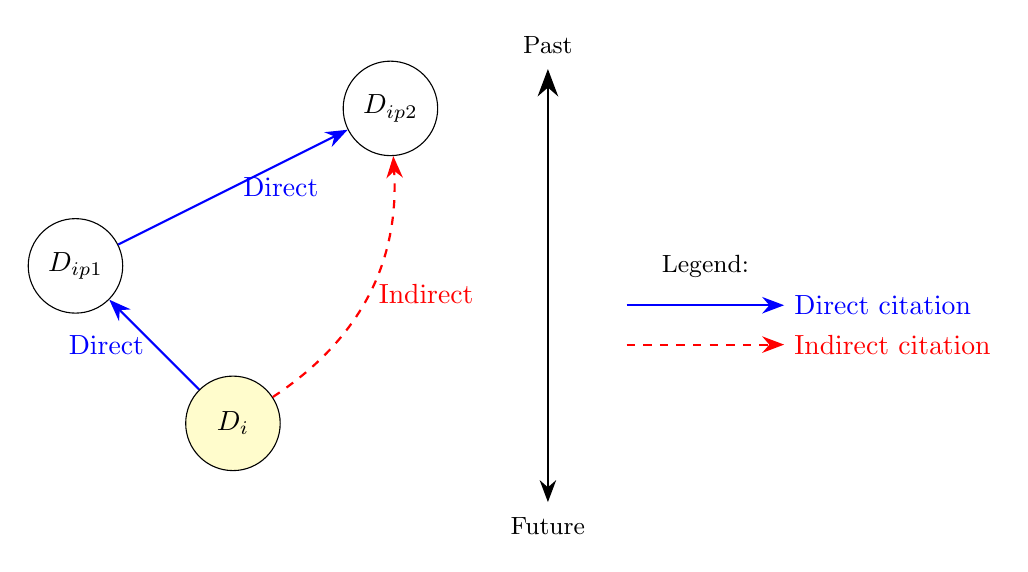
\begin{tikzpicture}[
        > = {Stealth[scale=1.2]},
        vertex/.style = {circle, draw, minimum size=1.2cm, inner sep=1pt},
        ref_edge/.style = {->, thick, blue},
        indirect_edge/.style = {->, thick, red, dashed},
        label_style/.style = {font=\small}
    ]
    
    % Main document Di
    \node[vertex, fill=yellow!20] (Di) at (0,0) {$D_i$};
    
    % Direct reference
    \node[vertex] (Dip1) at (-2,2) {$D_{ip1}$};
    
    % Indirect reference
    \node[vertex] (Dip2) at (2,4) {$D_{ip2}$};
    
    % Add edges
    \draw[ref_edge] (Di) -- (Dip1) node[midway, left] {Direct};
    \draw[ref_edge] (Dip1) -- (Dip2) node[midway, right] {Direct};
    \draw[indirect_edge] (Di) to[bend right] node[midway, right] {Indirect} (Dip2);
    
    % Time arrow (vertical)
    \draw[{Stealth[scale=1.5]}->, thick] (4,4.5) -- (4,-1);
    \node[label_style] at (4,4.8) {Past};
    \node[label_style] at (4,-1.3) {Future};
    
    % Legend
    \node[label_style] at (6,2) {Legend:};
    \draw[ref_edge] (5,1.5) -- (7,1.5) node[right] {Direct citation};
    \draw[indirect_edge] (5,1) -- (7,1) node[right] {Indirect citation};

    \end{tikzpicture}

    
    \caption{Demonstration of an indirect citation. $D_i$ is related to $D_{ip2}$ yet only through $D_{ip1}$. This can occur for single nodes or entire components. }
    \label{fig:indirect-citation}
\end{figure}

Research addressing this limitation was analysed, and these potential solutions exist to address this limitation:

\begin{itemize}
    \item \textbf{Matching isolated nodes based on similarity metric of their embeddings}: If $N$ is all the documents in the total pool, and $N_{isolated}$ is the set of documents that are not cited by any other document in $N$, then for each document $D_{ip} \in N_{isolated}$, find the document $D_i \in N$ with the highest similarity metric (i.e. cosine similarity) to $D_{ip}$. Add an artificial edge between $D_i$ and $D_{ip}$.
    \item \textbf{Matching isolated components on similarity metric of their embeddings}: Some small groups of documents (called isolated components) may be disconnected from the main cluster when analysing document clusters. These isolated components have fewer connections to other documents, which can reduce classification accuracy. To fix this:
    \begin{itemize}
        \item Identify isolated components $C_{isolated}$ that have fewer or equal nodes than the main cluster.
        \item For each node in these isolated components.
        \item Calculate a similarity metric (i.e. cosine similarity) to nodes in larger clusters $C_i$.
        \item Connect it to the most similar large cluster by adding an artificial edge.
    \end{itemize}

\end{itemize}



Even without these potential fixes, node isolation does not prevent \gls*{bcs} or \gls*{fcs} augmenting the title and abstract screening \gls*{cal} process. Assessing the citation network of the seed document(s) can potentially provide a strong signal to improve recall in the early screening stages.

\subsubsection{Work completed towards RQ1}

\paragraph{Quantifying the \gls*{bcs} citation mining signal:}
The strength of the \gls*{bcs} signal was quantified through a pilot experiment designed to quantify the ratio of relevant documents directly citing other relevant documents, leveraging the OpenAlex API. For each document in the pool of the \gls*{clef} 2019 \gls*{dta} dataset, the OpenAlexAPI was used to retrieve its references, and these references were filtered to include only those documents that were in the total pool. Then, three groups of ``seed” documents were sampled for comparative analysis: a positive group (up to 100 documents labelled as relevant), a negative group (up to 100 documents labelled as irrelevant), and a random group (100 documents selected at random from the total pool). The total count of its one-hop cited references marked as relevant or not relevant was calculated for each seed document. The counts of relevant (true) and irrelevant (false) citations were aggregated across the eight systematic reviews. Z-tests for proportions were performed to compare the three groups, and the differences were visualised using stacked bar charts (with 95\% confidence intervals computed via a normal approximation). The results show that the positive seed group exhibited a higher proportion of one-hop relevant citations (0.28) compared to both the negative (0.14) and random groups (0.17) - See Figure \ref{fig:bcs_experiement}, with statistical tests (e.g., z-statistics over 11 and p-values $\leq$ 0.001) confirming that these differences were highly significant.


\begin{figure}
    \centering
    \includesvg[width=1\linewidth]{Confirmation Review/images/relatedness.svg}
    \caption{Ratio of one-hop relevance ratio from starting seeds}
    \label{fig:bcs_experiement}
\end{figure}



\paragraph{Replication of Encoder-CAL approach:}
Mao's study~\cite{mao_reproducibility_2024}, where an Encoder \gls*{cal} approach was used in the \gls*{cal} process was recreated by the author, except the larger $\text{BioLinkBERT}_{\text{large}}$ formed the classifier. The larger model achieved higher performance in R-Precision in 7 of 12 datasets/policy combinations. The Friedman test for individual datasets found significant differences between the FPT epochs 4 out of 12 times; however, when considering all datasets together, there was no significant difference between the FPT epochs and R-precision for relevant selection policy or uncertainty selection policy. Original Encoder-CAL research investigated the ``Goldilocks problem", which essentially posited an ``optimum" number of further pertaining epochs needed on encoder-based models to achieve good performance. The research conducted by the author and Mao demonstrates that the ``Goldilocks problem", while present in non-medical domains, is not apparent when using the BiolinkBERT models for the \gls*{clef} dataset within a \gls*{cal} process, indicating that further pre-training of models was unnecessary as it does not produce a statistically significant improvement in R-precision. The average R-precision of each FPT epoch is reported in Table \ref{tab:results}, with the highest R-precision for relevancy selection policy being 0.847 at further pretrain epoch two and the highest R-precision for uncertainty being 0.832 at further pretrain epoch 1.  

Key findings from this exploratory research are that an optimal pre-training epoch is unlikely to be found within the \gls*{clef} dataset and, hence, not a viable avenue for future research. This is also of great practical importance to this PhD, as it removes the need for the computationally costly model further pre-training.  In terms of experimental design, certain hyperparameters were chosen without clear reasoning (such as batch size being 25, fine-tuning for 20 epochs and stopping after 501 documents labelled). This limitation is considered a barrier to improving the performance of the encoder \gls*{cal} process within that experimental framework, given that reported R-Precision values are already close to the natural ceiling of 1 (with R-Precision reaching 0.945 in some cases). Furthermore, using a more performance/larger model will likely be fruitful for future research. However, it depends on the availability and development of superior models (the creation of which is unfeasible during a PhD period). This undertaken research did, however, highlight that leveraging citations themselves was valuable to the \gls*{cal} process. 

\begin{table}[htbp]
    \centering
    \footnotesize
    \setlength{\tabcolsep}{4pt}
    \begin{tabular}{l>{\raggedright\arraybackslash}p{1.2cm}ccccc}
    \hline
    \textbf{Collection} & \textbf{Dataset size} & \textbf{Model} & \multicolumn{2}{c}{\textbf{R-Precision (↑)}} & \multicolumn{2}{c}{\textbf{Friedman (p)}} \\
    \cline{4-7}
    & & & \textbf{Rel.} & \textbf{Unc.} & \textbf{Rel.} & \textbf{Unc.} \\
    \hline
    \multirow{6}{*}{\makecell[l]{\gls*{clef} 2019\\dta test}} & 
    \multirow{6}{*}{8} & BiolinkBert-Base-ep0 & \textbf{0.909} & \textbf{0.857} & \multicolumn{2}{c}{---} \\
    & & BiolinkBert-Large-ep0 & 0.897 & 0.803 & \multirow{5}{*}{0.914} & \multirow{5}{*}{0.632} \\
    & & BiolinkBert-Large-ep1 & 0.827 & 0.832 & & \\
    & & BiolinkBert-Large-ep2 & 0.812 & 0.774 & & \\
    & & BiolinkBert-Large-ep5 & 0.841 & 0.814 & & \\
    & & BiolinkBert-Large-ep10 & 0.881 & 0.846 & & \\
    \hline
    \multirow{6}{*}{\makecell[l]{\gls*{clef} 2017\\test}} & 
    \multirow{6}{*}{30} & BiolinkBert-Base-ep0 & 0.812 & 0.794 & \multicolumn{2}{c}{---} \\
    & & BiolinkBert-Large-ep0 & 0.828 & 0.797 & \multirow{5}{*}{\textbf{\textless0.05}} & \multirow{5}{*}{\textbf{\textless0.05}} \\
    & & BiolinkBert-Large-ep1 & 0.826 & \textbf{0.827} & & \\
    & & BiolinkBert-Large-ep2 & \textbf{0.858} & 0.804 & & \\
    & & BiolinkBert-Large-ep5 & 0.827 & 0.777 & & \\
    & & BiolinkBert-Large-ep10 & 0.799 & 0.757 & & \\
    \hline
    \multirow{6}{*}{\makecell[l]{\gls*{clef} 2017\\train}} & 
    \multirow{6}{*}{20} & BiolinkBert-Base-ep0 & \textbf{0.838} & 0.761 & \multicolumn{2}{c}{---} \\
    & & BiolinkBert-Large-ep0 & 0.778 & 0.765 & \multirow{5}{*}{\textbf{\textless0.05}} & \multirow{5}{*}{0.28} \\
    & & BiolinkBert-Large-ep1 & 0.808 & 0.789 & & \\
    & & BiolinkBert-Large-ep2 & 0.767 & 0.701 & & \\
    & & BiolinkBert-Large-ep5 & 0.816 & 0.786 & & \\
    & & BiolinkBert-Large-ep10 & 0.827 & \textbf{0.796} & & \\
    \hline
    \multirow{6}{*}{\makecell[l]{\gls*{clef} 2018\\test}} & 
    \multirow{6}{*}{30} & BiolinkBert-Base-ep0 & 0.794 & 0.780 & \multicolumn{2}{c}{---} \\
    & & BiolinkBert-Large-ep0 & 0.789 & 0.774 & \multirow{5}{*}{0.52} & \multirow{5}{*}{0.50} \\
    & & BiolinkBert-Large-ep1 & \textbf{0.812} & 0.790 & & \\
    & & BiolinkBert-Large-ep2 & 0.797 & \textbf{0.791} & & \\
    & & BiolinkBert-Large-ep5 & 0.763 & 0.773 & & \\
    & & BiolinkBert-Large-ep10 & 0.763 & 0.769 & & \\
    \hline
    \multirow{6}{*}{\makecell[l]{\gls*{clef} 2019\\\gls*{dta} int.\\train}} & 
    \multirow{6}{*}{20} & BiolinkBert-Base-ep0 & 0.939 & 0.923 & \multicolumn{2}{c}{---} \\
    & & BiolinkBert-Large-ep0 & 0.939 & 0.902 & \multirow{5}{*}{0.78} & \multirow{5}{*}{0.50} \\
    & & BiolinkBert-Large-ep1 & 0.941 & 0.935 & & \\
    & & BiolinkBert-Large-ep2 & 0.948 & 0.921 & & \\
    & & BiolinkBert-Large-ep5 & 0.952 & 0.945 & & \\
    & & BiolinkBert-Large-ep10 & \textbf{0.945} & \textbf{0.947} & & \\
    \hline
    \multirow{6}{*}{\makecell[l]{\gls*{clef} 2019\\\gls*{dta} int.\\test}} & 
    \multirow{6}{*}{20} & BiolinkBert-Base-ep0 & \textbf{0.934} & \textbf{0.900} & \multicolumn{2}{c}{---} \\
    & & BiolinkBert-Large-ep0 & 0.899 & 0.856 & \multirow{5}{*}{0.87} & \multirow{5}{*}{\textbf{\textless0.05}} \\
    & & BiolinkBert-Large-ep1 & 0.904 & 0.840 & & \\
    & & BiolinkBert-Large-ep2 & 0.909 & 0.878 & & \\
    & & BiolinkBert-Large-ep5 & 0.882 & 0.835 & & \\
    & & BiolinkBert-Large-ep10 & 0.865 & 0.841 & & \\
    \hline
   
    \end{tabular}
    \caption{Performance comparison across different collections and models}
    \label{tab:results}
\end{table}


\subsubsection{Experimental approach}

The proposed initial experiment evaluates if prioritising one-hop away from a known relevant document improves \gls*{cal} for Title and Abstract Screening. To do this, a Relation-Prioritised \gls*{cal} (RP-CAL) approach will be compared with Baseline \gls*{cal} (B-CAL) approaches. 

To understand the RP-CAL approach, consider the \gls*{cal} process output at each active learning iteration to understand the approach. A sigmoid value from a model trained on the known data pool determines document ranking where a policy selects relevant samples. Exceptions to this are revealed documents; a score of infinity is assigned if relevant to the search, and negative infinity is assigned if not. Figure \ref{fig:document_ranking_iteration} provides a simple outline of this process.

\begin{figure}[h!]
\centering

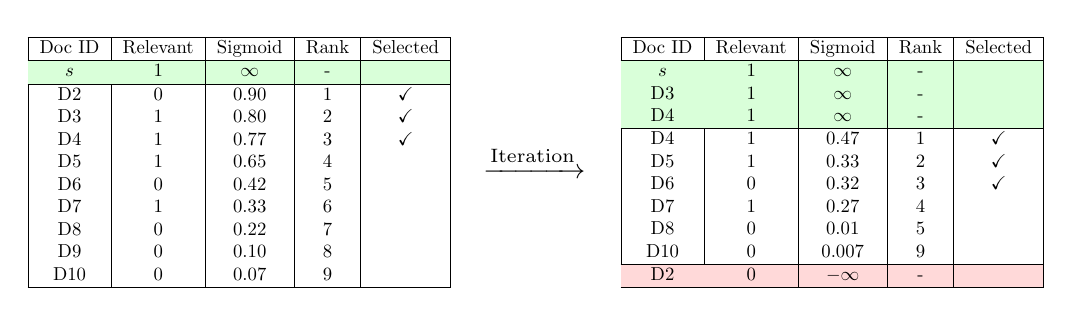
\begin{tikzpicture}[node distance=0.2cm]  % Adjust space between nodes here
\node (table1) [inner sep=0pt] {
\resizebox{0.45\textwidth}{!}{%  <-- 40% width
\begin{tabular}{|c|c|c|c|c|}
\hline
Doc ID & Relevant & Sigmoid & Rank & Selected \\
\hline
\rowcolor{green!15}
$s$ & 1 & $\infty$ & - &  \\
\hline
D2 & 0 & 0.90 & 1 & \checkmark \\
D3 & 1 & 0.80 & 2 & \checkmark\\
D4 & 1 & 0.77 & 3 & \checkmark \\
D5 & 1 & 0.65 & 4 &  \\
D6 & 0 & 0.42 & 5 &  \\
D7 & 1 & 0.33 & 6 &  \\
D8 & 0 & 0.22 & 7 &  \\
D9 & 0 & 0.10 & 8 &  \\
D10 & 0 & 0.07 & 9 &  \\
\hline
\end{tabular}
}
};

\node (arrow) [right=of table1] {$\xrightarrow{\text{Iteration}}$};

\node (table2) [right=of arrow] {
\resizebox{0.45\textwidth}{!}{% <-- 40% width
\begin{tabular}{|c|c|c|c|c|}
\hline
Doc ID & Relevant & Sigmoid & Rank & Selected \\
\hline
\rowcolor{green!15}
$s$ & 1 & $\infty$ & - &  \\
\rowcolor{green!15}
D3 & 1 & $\infty$ & - &  \\
\rowcolor{green!15}
D4 & 1 & $\infty$ & - & \\
\hline
D4 & 1 & 0.47 & 1 & \checkmark \\
D5 & 1 & 0.33 & 2 &  \checkmark\\
D6 & 0 & 0.32 & 3 & \checkmark \\
D7 & 1 & 0.27 & 4 &  \\
D8 & 0 & 0.01 & 5 &  \\
D10 & 0 & 0.007 & 9 &  \\
\hline
\rowcolor{red!15}
D2 & 0 & $-\infty$ & - &  \\
\hline
\end{tabular}
}
};
\end{tikzpicture}

\caption{Document ranking and selection before and after an Active Learning iteration. Note that the selection policy used here is relevance with a batch size of 3.}
\label{fig:document_ranking_iteration}
\end{figure}

In the \gls*{cal} process, one or more relevant seed documents, denoted $s$, are first identified. From these seeds, document relationships to the entire pool, $\textbf{T}$ can be extracted (e.g., via OpenAlex). A simple document relationship is if a document $d$ in $\textbf{T}$ are reachable from $s$, within $n$ hops (where a \emph{hop} indicates the number of edges traversed on a \gls*{gnn} using \gls*{bcs} or \gls*{fcs} as edges). This could be returned as set for the $s$, as outlined in Equation \ref{eq:related_eq}.

\begin{equation}
    O_{n_{(s)}} = Related(s, n,\textbf{T})
   \label{eq:related_eq} 
\end{equation}

The goal is to make the \gls*{cal} ranking procedure \emph{relationship‐aware} by giving preference to $O_{n(s)}$ over $\textbf{T} \setminus {n(s)} $. The sigmoid output (bounded by 0 and 1) used to score each document can be adjusted. This can be achieved through an indicator function to identify whether a document $d$ is in the relationship set $O_{n(s)}$ - shown in Equation \ref{eq:Indicator_function_ons}.

\begin{equation}
    {I_{O_{n(s)}}(d) = \begin{cases}
1 & \text{if } d \in O_{n(s)} \\
0 & \text{otherwise }
\end{cases}}
\label{eq:Indicator_function_ons}
\end{equation}

Let X be the original sigmoid output (or any scoring function). This score is adjusted using a scaling factor $\alpha \in [-1, 1]$ to control the influence of the relationship information - as shown in Equation \ref{eq:Adjusted_score}:

\begin{equation}
\text{Adjusted Score}_{(d)} = X(d) \cdot(1+\alpha I_{O_{n{(s0)}}}(d))
\label{eq:Adjusted_score}
\end{equation}
When $\alpha > 0$, documents in $O_{n(s)}$ receive a higher score; when $\alpha < 0$, they receive a lower score.

An RP-CAL approach using \cite{mao_reproducibility_2024}'s encoder-CAL method and \cite{cormack_scalability_2016}'s BMI will be compared to a B-CAL approach that is not relationship-aware (i.e., the default \cite{mao_reproducibility_2024} and \cite{cormack_scalability_2016} approach).   

This approach can be expanded further by making the \gls*{cal} process aware of other document relations. You can, for example, use the RA-CAL approach to consider the highest-cited documents more preferentially or authors who appear most in the $\textbf{T}$. It can be used on any \gls*{cal} approach as it utilises the model output (score). 

\paragraph{Experimental variations:}
The experimental design can incorporate several key variations to understand the impact of different parameters on \gls*{cal} performance. Seed size selection is likely to be highly impactful (i.e., vary how many positive cases the RP-CAL process starts with compared to the B-CAL). This is likely to be due to the larger $O_{n{(s)}}$ size. Additionally, you can continually update the $O_{n{(s)}}$ set, as when more positive document classifications come along, you can extend this set with the updated pool. The contribution of each citation searching approach of \gls*{bcs}, (i.e., form $O_{n{(s)}}$ using only \gls*{bcs}, RP-CAL-BCS), \gls*{fcs} (i.e., form $O_{n{(s)}}$ using only \gls*{fcs}, RP-CAL-FCS) can be compared to using both \gls*{bcs}+\gls*{fcs} (RP-CAL-BCS+FCS). Finally, the effect of network expansion can be assessed by evaluating the effectiveness of the best-performing RP-CAL approaches that are one hop away versus two or three hops away.  


\begin{figure}[h!]
\centering

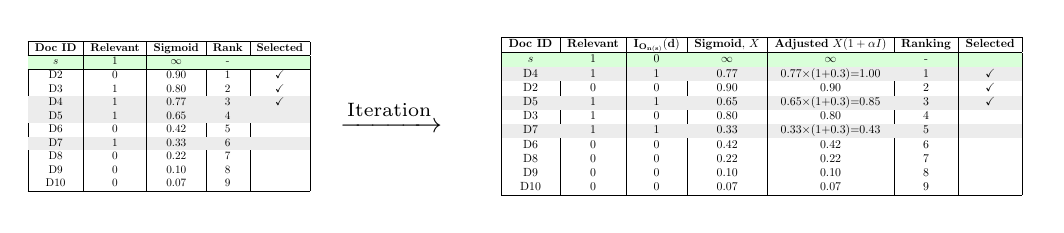
\begin{tikzpicture}[node distance=0.2cm]  % Adjust space between nodes here
\node (table1) [inner sep=0pt] {
\resizebox{0.3\textwidth}{!}{%  <-- 40% width
\begin{tabular}{|c|c|c|c|c|}
\hline
\textbf{Doc ID} & \textbf{Relevant} & \textbf{Sigmoid} & \textbf{Rank} & \textbf{Selected} \\
\hline
\rowcolor{green!15}
$s$ & 1 & $\infty$ & - &  \\
\hline
D2 & 0 & 0.90 & 1 & \checkmark \\
D3 & 1 & 0.80 & 2 & \checkmark\\
\rowcolor{gray!15}
D4 & 1 & 0.77 & 3 & \checkmark \\
\rowcolor{gray!15}
D5 & 1 & 0.65 & 4 &  \\
D6 & 0 & 0.42 & 5 &  \\
\rowcolor{gray!15}
D7 & 1 & 0.33 & 6 &  \\
D8 & 0 & 0.22 & 7 &  \\
D9 & 0 & 0.10 & 8 &  \\
D10 & 0 & 0.07 & 9 &  \\
\hline
\end{tabular}
}
};

\node (arrow) [right=of table1] {$\xrightarrow{\text{Iteration}}$};

%----------- RIGHT TABLE: Relationship-aware CAL -----------
\node (table2) [right=of arrow, xshift=0.3cm] {
\resizebox{0.55\textwidth}{!}{%
\begin{tabular}{|c|c|c|c|c|c|c|}
\hline
\textbf{Doc ID} & \textbf{Relevant} 
  & \(\mathbf{I_{O_{n(s)}}(d)}\)
  & \textbf{Sigmoid}, $X$
  & \textbf{Adjusted} $X(1 + \alpha I)$
  & \textbf{Ranking}
  & \textbf{Selected}\\
\hline
\rowcolor{green!15}
$s$ & 1 & 0 & $\infty$ & $\infty$ & - &   \\

\hline

\rowcolor{gray!15}
D4 & 1 & 1 & 0.77 & 0.77$\times$(1+0.3)=1.00 & 1 & \checkmark \\
D2 & 0 & 0 & 0.90 & 0.90 & 2 & \checkmark \\
\rowcolor{gray!15}
D5 & 1 & 1 & 0.65 & 0.65$\times$(1+0.3)=0.85 & 3& \checkmark \\
D3 & 1 & 0 & 0.80 & 0.80 & 4 & \\
\rowcolor{gray!15}
D7 & 1 & 1 & 0.33 & 0.33$\times$(1+0.3)=0.43 & 5&  \\
D6 & 0 & 0 & 0.42 & 0.42 & 6&  \\
D8 & 0 & 0 & 0.22 & 0.22 & 7&  \\
D9 & 0 & 0 & 0.10 & 0.10 & 8&  \\
D10 & 0 & 0 & 0.07 & 0.07 & 9 &  \\

\hline
\end{tabular}
}
};
\end{tikzpicture}

\caption{Effect of relationship‐aware CAL when $O_{n(s)} = {D4, D5, D7}$ (rows highlighted grey) are in  with $\alpha = 0.3$. Scores are boosted by a factor of $(1+\alpha)$ if $I_{O_{n(s)}}(d)=1$, causing  $O_{n(s)}$ to rise in ranking.}
\label{fig:relationship_aware_example}
\end{figure}

\paragraph{Hyperparameters:}
Existing hyperparameter choices (e.g., batch size, learning rates, fine-tuning epochs or active learning iterations) can be taken from the existing implementation or form part of the experimental research. To begin with, a broad range of $\alpha$ will be examined to see if RP-CAL improves efficiency over BE-CAL. Setting $\alpha$ to zero would revert the \gls*{cal} approach to the standard approach. Optimal settings potentially for $\alpha$ exist across all systematic reviews, depending on the relationship examined. Extension work for this experiment could look at ways to automate finding these (e.g., using the variance in the feature to set $\alpha$, with greater variance indicating potential greater $\alpha$ needed, reinforcement learning techniques, or clustering techniques).

\paragraph{Evaluation:}
The performance of these approaches will be evaluated on the \gls*{clef}-\gls*{tar} (2017, 2018, 2019) and Synergy datasets. To combat any effect of title and abstract updating, this PhD will use a recently collected set \(2024\) of titles/abstracts created by Mao et al.~\cite{mao_reproducibility_2024} for the \gls*{clef} dataset\footnote{https://github.com/ielab/goldilocks-reproduce}. Success will be measured through several performance metrics, including Recall@95\%, R-Precision, WSS@95\%. Statistical analyses (e.g., paired t-tests) will assess whether the observed differences between RP-CAL approaches and the B-CAL approach are significant.

\subsection{Question 2: Leveraging metadata for \gls*{cal}}
\begin{tcolorbox}[colback=lightgreen!10, colframe=lightgreen, sharp corners=southwest, boxrule=0.8pt]
\emph{\textbf{How does incorporating structured article metadata (e.g., publication date, author information, citation counts) into document representations using \gls*{gnn} architectures affect the efficiency and accuracy of document prioritisation in \gls*{cal} for medical systematic reviews, compared to traditional approaches?}}
\end{tcolorbox}

The aim is to determine if creating document representations enriched with metadata leads to higher recall rates, improved R-Precision, and reduced overall human screening workload.

\subsubsection{Experimental Approach} 

To evaluate the benefits of metadata integration, a comparative study involving three groups is proposed:

\begin{enumerate} \item \textbf{Baseline \gls*{cal} (BE-CAL)\cite{mao_reproducibility_2024}:}
This approach uses a standard encoder model (e.g., BioLinkBERT) that encodes each document’s title and abstract into a fixed-size (e.g., 768-dimensional) vector derived from the [CLS] token. This representation is then used within the active learning loop for ranking and selection.

\item \textbf{\gls*{gnn}-based Document Representation without Metadata (\gls*{gnn}-DR):}
In this model, a document graph is constructed based solely on text features (titles and abstracts) and inter-document connectivity (e.g., citation links). A \gls*{gnn} (using an architecture such as \glspl*{gcn}, \glspl*{gat}, or GraphSAGE) is then applied to derive node embeddings (for example, 128-dimensional vectors) that capture textual content and connectivity. 

\item \textbf{\gls*{gnn}-based Document Representation with Metadata (\gls*{gnn}-DR+Meta):}
Here, node features are enriched by concatenating the text-based embedding (e.g., from a \gls*{bert}-based model) with structured metadata. For instance, the initial feature vector for a document might be represented as:


\[
[\underbrace{\mathrm{\gls*{bert}}_{768}}_{\text {title+abstract }}, \underbrace{\text { Year }}_{\text{Publication Year}}, \underbrace{\text { JournalID }}_{\text{journal identifier}} , \underbrace{\text { Citation Count }}_{\text{citation count}} ,\ldots] 
\]

\vspace{0.5em}

The \gls*{gnn} is then applied to this enriched graph to produce improved node embeddings incorporating textual, relational, and metadata signals. \end{enumerate}

Each representation group will form the different experimental arms, and each will feed into the \gls*{cal} pipeline. A classifier model (e.g., logistic regression) will use these inputs to iteratively rank unlabelled documents in a \gls*{cal} setting on the \gls*{clef}-\gls*{tar}(2017, 2018, 2019) and Synergy datasets.  Performance will be measured using Recall@95\%, R-Precision, and \gls*{wssk} metrics.

\paragraph{Experimental variations:}
Further extensions can occur to understand key choices about this experimental design. An ablation study could assess the relative contribution of individual metadata features (e.g., publication year, author names, journal identifiers). This will help determine the most informative features. Experiments can be conducted with different dimensions (e.g., 128, 256, 512) for the \gls*{gnn}-derived node embeddings to balance the representational dimensions and computational efficiency. Overstuffing can potentially occur in lower dimensions. Experiments can be conducted with different variations for $k$ (e.g., 1, 2, 5, 10) for the \gls*{gnn}-derived node embeddings. Increasing $k$ values will increase the amount of ``relational" data shared between each node (document representation). High values of $k$ will result in a fully receptive field (in other words, every node is updated using information from every other node). This could result in over-smoothing, where node representations become too similar, or over-squashing, where too much information from many nodes is compressed into a fixed embedding dimension. Different message-passing architectures (e.g., \glspl*{gcn}, \glspl*{gat} or GraphSAGE) can be compared to determine which best captures the combined signals from text and metadata.

\paragraph{Evaluation:}
Will be the same as per RQ1. 

\subsection{Question 3: Informing stopping decisions with information utility}

\begin{tcolorbox}[colback=salmon!10, colframe=salmon, sharp corners=southwest, boxrule=0.8pt]
\emph{\textbf{How do stopping criteria based on the utility of retrieved information (aligned with user information needs) influence the total manual screening workload in \gls*{cal} for systematic reviews, and how do these criteria compare with conventional recall-based stopping rules?}}
\end{tcolorbox}

Rather than enforcing a strict recall target, \emph{utility-based} stopping seeks to halt once the pool of included documents collectively provides enough evidence to address the research question. 

\subsubsection{Work completed towards RQ3}

To extend this research area, the author has submitted work for peer review that measures information utility through moments of a probability distribution, along with a decision threshold to reduce screening of relevant documents. This was submitted to the SIGIR 2025 conference\footnote{https://sigir2025.dei.unipd.it} and is under peer review. This work introduces a novel utility-based approach to stopping rules for medical literature screening within \gls*{tar}. Moving beyond traditional recall-based methods, this work focuses on halting the search process based on the utility of the information retrieved thus far, specifically its value in answering the underlying research question (modelled as a decision threshold). Several new algorithms were developed, leveraging the statistical concept of moments of a probability distribution: Harmonic Shrinkage, Confidence Boundary, Skewness, Kurtosis, and Multi-Moments. Experiments demonstrated that the Confidence Boundary algorithm achieves high decision agreement with significantly reduced document review compared to target-recall approaches. This research supports this PhD's goal of improving efficiency in the medical screening process by offering a more efficient and reasoning-based approach, aligning stopping decisions with the actual information needs of the user. As this has already been submitted (and contributed to this research question), further experimental avenues are discussed in this section.   

\subsubsection{Experimental Approach}

Limitations of the author's previous work lie in that the approaches were only applied to \gls*{dta}. \gls*{dta} were chosen as the point estimates primary research reports (i.e. sensitivity and false-positive rate) are easily interpretable. They can be combined into a single combined point estimate easily (via summing true positives, true negatives, false positives and false negatives across all research), values for which were available from the  Limsi-Cochrane Dataset~\cite{norman_cochrane_2018}. Although these utility-based methods proved successful in \gls*{dta}, other systematic reviews (e.g., interventional, prognostic, qualitative) may require different outcome measures or stopping criteria. A stopping method must be applied in various review types, such as interventional studies, to have a broad impact. 

The utility of interventional studies can be derived similarly through effect measures (a statistical construct that compares two outcome groups). Depending on the reported outcome data, different effect measures are reported within an interventional systematic review. If absolute values were reported, effect measures such as mean difference can be reported per study, or if ratios were measured, then a risk ratio could be reported. However, intervention studies are potentially even more suited to the approaches the Author created for \gls*{dta}; unlike them, effect measures all have a natural decision boundary ($\theta$), zero. 

Consider this standard mean difference chart from a systematic review in the \gls*{clef} 2019 intervention dataset, where one outcome measured was whether ultrasound guidance or infiltration is a better choice in nerve blocks in children (i.e., is group a or b a better intervention for this population) - see Figure \ref{fig:cochrane_ultrasound}, 1.2.3 Ultrasound vs Infiltration \cite{the_cochrane_collaboration_use_2014}.

\begin{figure}
    \centering
    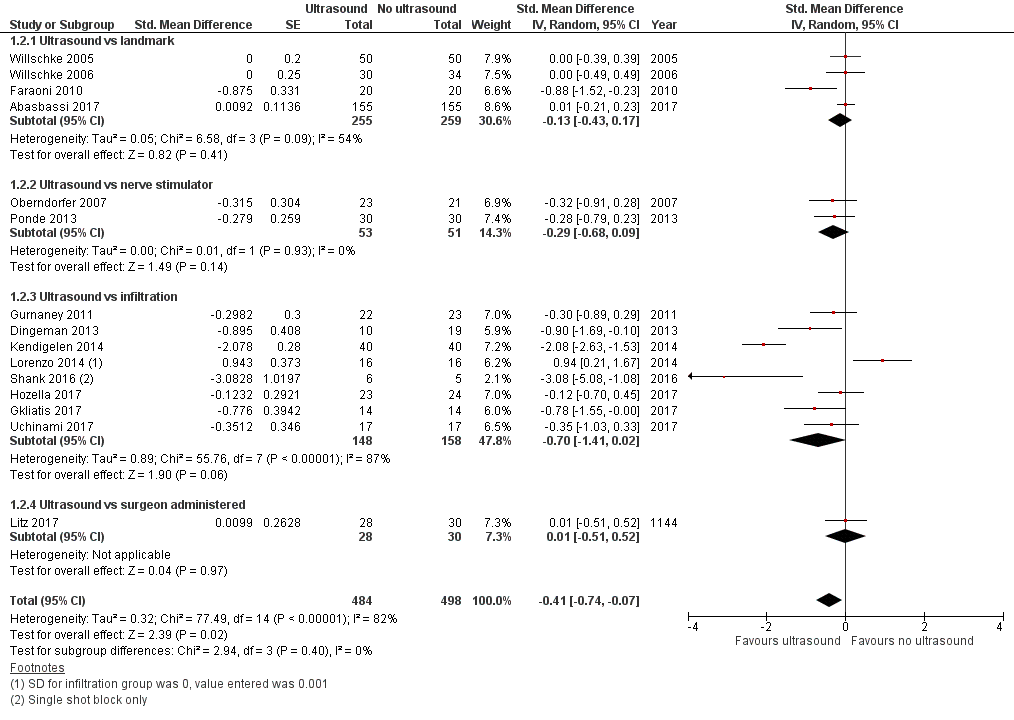
\includegraphics[width=1\linewidth]{Confirmation Review/images/cochrane_ultrasound.png}
    \caption{Effect measures of multiple outcomes in a single Cochrane review~\cite{norman_cochrane_2018}. The black diamond's overall effect size is determined after examining all information.\protect\footnotemark}
    \label{fig:cochrane_ultrasound}
\end{figure}

\footnotetext{Reproduced from~\cite{norman_cochrane_2018} under the CC BY 4.0 license \url{https://creativecommons.org/licenses/by/4.0/}. No changes were made.}

Using the same approaches as in the Author's work on Utility-based stopping, stopping rules considering confidence boundaries crossing this $\theta = 0$ or a harmonic shrinkage-based approach can be devised~\cite{lau_cumulative_1992}. For example, once the lower confidence boundary for accumulated information for recalled studies is above zero or the upper confidence boundary is below. This will be compared against the decision made with all information (i.e., the decision agreement metrics as outlined in the Author's utility work). This can be achieved using the confidence interval approach by calculating the confidence intervals around the effect measures after recalling each relevant document and stopping when the confidence intervals of the effect measures of each group no longer intersect.

A standard error (SE) and standard mean difference (SMD) are needed to calculate a confidence interval. The author took values for the outcome - each study ($i$) the SMD and SE to demonstrate the confidence boundary approach. The cumulative SMD up to study $k$ was calculated as in Equation \ref{eq:cumulativeSMD}:

\begin{equation}
    \text{Cumulative SMD}_k = \frac{\sum^k_{i=1} \frac{SMD_i}{SE^2_i}}{\sum^k_{i=1} \frac{1}{SE^2_i}}
    \label{eq:cumulativeSMD}
\end{equation}

The cumulative standard error was calculated using Equation \ref{eq:cumulativeSE}:

\begin{equation}
    \text{SE}_k = \sqrt{\frac{1}{\sum^k_{i=1} \frac{1}{SE^2_i}}}
    \label{eq:cumulativeSE}
\end{equation}


The 95\% confidence interval is calculated as in Equation \ref{eq:ci}.

\begin{equation}
    \text{Upper/Lower Bound}_k = \text{Cumulative SMD}_k \pm 1.96 \cdot SE_k
    \label{eq:ci}
\end{equation}

Plotting the Cumulative SMD over time, see Figure \ref{fig:culm_smd}, shows that if you order the studies in the way they have screened the studies in the order they were presented in the paper (year), that \gls*{ir} could have been terminated after the second study, as enough information utility was available to answer the question that ultrasound is favoured. 

\begin{figure}
    \centering
    \includesvg[width=1\linewidth]{Confirmation Review/images/cochrane_utility.svg}
    \caption{Demonstration of how to use an effect measure to derive stopping index. In the second study, the upper confidence boundaries derived from information up to study 2 is below $\theta$.}
    \label{fig:culm_smd}
\end{figure}

There is a clear ability to reduce information recall, even if the information is presented in different orders. Even if the study order is randomly permuted (and hence, their contribution to the SMD is randomised), enough information has been obtained by study 5 to terminate recall -  see Figure \ref{fig:aggrevated_stop}.

\begin{figure}
    \centering
    \includesvg[width=1\linewidth]{Confirmation Review/images/aggrevated_stopping.svg}
    \caption{Demonstration of how to use an effect measure to derive stopping index. In the fifth study, the upper confidence boundaries derived from information up to study 2 is below $\theta$.}
    \label{fig:aggrevated_stop}
\end{figure}

To achieve this, additional data must be created to augment the \gls*{clef} 2019 Intervention Reviews and Synergy Datasets. This process can be completed quickly through optical character recognition (as done with the Limsi-Cochrane dataset and by the Author in the Utility-Based Stopping Methods paper) and manual verification. Additionally, collating the true positives, false positives, true negatives, and false negatives from medical systematic reviews included in the Synergy dataset would allow a greater dataset to establish further the generalisability of the already presented utility-based stopping rules.

Studies would be screened according to their ranking within AuthTAR (which is pre-existing). The effectiveness of utility-based methods, as adapted for the intervention datasets, will be compared against existing baseline approaches (such as fixed-recall targets or reinforcement learning-based approaches).

\paragraph{Experimental variations:}
 Extensions to the stopping rules would more extensively consider the total population of included patients. In the original research, the Confidence Boundary, Skewness and Kurtosis rules did consider the total population of included patients tangentially - i.e., the bigger the population, the smaller the margin of error of the confidence intervals are likely to be. However, the integration of total participants could be more explicit. It has been long established that sample size calculations (e.g., the minimum number of patients required to demonstrate the difference between two intervention groups) could be examined further - should stopping be able to occur before that threshold is met across multiple pieces of research? 

\paragraph{Evaluation:}
Would utilise the author's previous research evaluation metrics. Efficiency will be measured through the \gls*{prd}  alongside a traditional savings metric. Effectiveness will be measured through Decision agreement (a binary indicator function determining if the decision made at stopping matches the decision made with all available information). 




\section{Ethics statement}\label{sec:ethics}

This PhD research will utilise pre-existing, publicly available datasets for analysis. Crucially, this research does not involve any direct interaction with human participants, and no new data collection will be undertaken. The datasets being analysed consist of anonymised data from prior research, ensuring the privacy of the original participants is already protected. Therefore, this research poses minimal ethical risk, as it avoids direct engagement with human subjects and relies solely on data where identifiability has already been removed through prior anonymisation processes.

Furthermore, as this research re-uses existing data and archival data, its scope aligns with the University's ethical guidelines in Policy Note No. 13. Policy Note No. 9 respectively\footnote{https://students.sheffield.ac.uk/research-ethics/ethics/notes/policy-note-13}\footnote{https://students.sheffield.ac.uk/research-ethics/ethics/notes/policy-note-9}. Given these factors and by these policies, formal ethics approval was deemed unnecessary and has not been sought for this project.
\section{Data management plan}

A data management plan has been created for this PhD period and included in Appendix \ref{app:dmp}.


\section{Timeline}

A timeline for this PhD is presented in Gantt formation in Figure \ref{fig:gantt}. This timetable needs to be flexible and will likely change. More detail on each research task is outlined in for each Research Question in Tables \ref{tab:taskoverview_rq1}, \ref{tab:taskoverview_rq2} \& \ref{tab:taskoverview_rq3}.


\begin{figure}
    \centering
    \includesvg[width=1\linewidth]{Confirmation Review/images/gantt.svg}
    \caption{Projected PhD timeline in Gantt chart format.}
    \label{fig:gantt}
\end{figure}


\begin{sidewaystable}[htbp]
\centering
\small
\setlength{\extrarowheight}{2pt} % extra spacing between rows
\renewcommand{\arraystretch}{1.2} % increase overall row height

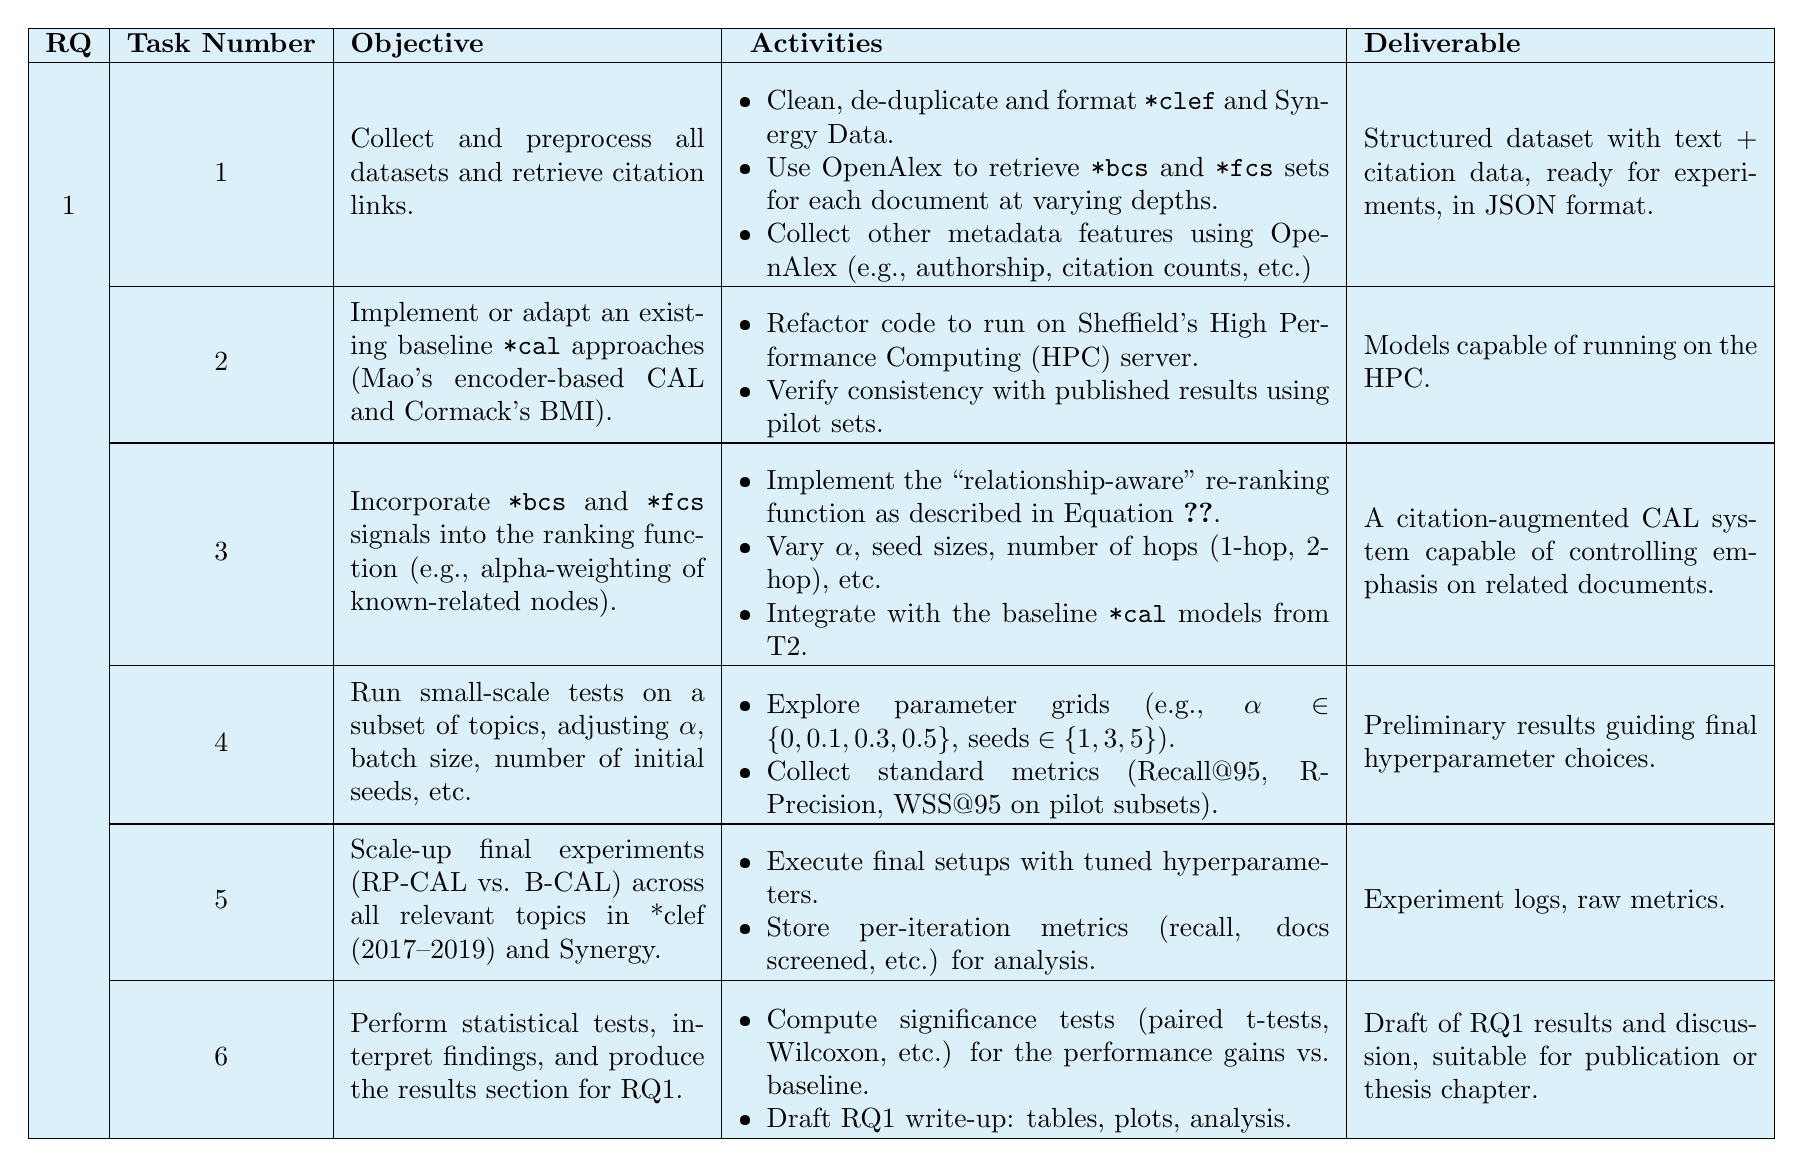
\begin{tikzpicture}
\node[fill=skyblue, fill opacity=0.3, text opacity=1, inner sep=0pt] {

\begin{tabular}{|c|c|m{4.5cm}|m{7.5cm}|m{5.0cm}|}
\hline
\textbf{RQ} & \textbf{Task Number} & \textbf{Objective }&\textbf{ Activities} & \textbf{Deliverable} \\
\hline
\multirow{3}{*}{1} 
  & 1 & Collect and preprocess all datasets and retrieve citation links. & 
  \vspace{1em}
      \begin{itemize}[nosep, leftmargin=*]
          \item Clean, de-duplicate and format \texttt{\gls*{clef}} and Synergy Data.
          \item Use OpenAlex to retrieve \texttt{\gls*{bcs}} and \texttt{\gls*{fcs}} sets for each document at varying depths.
          \item Collect other metadata features using OpenAlex (e.g., authorship, citation counts, etc.)
      \end{itemize}
  & Structured dataset with text + citation data, ready for experiments, in JSON format. \\
\cline{2-5}
  & 2 & Implement or adapt an existing baseline \texttt{\gls*{cal}} approaches (Mao's encoder-based CAL and Cormack's BMI). & 
  \vspace{1em}
      \begin{itemize}[nosep, leftmargin=*]
          \item Refactor code to run on Sheffield's High Performance Computing (HPC) server.
          \item Verify consistency with published results using pilot sets.
      \end{itemize}
  & Models capable of running on the HPC. \\
\cline{2-5}
  & 3 & Incorporate \texttt{\gls*{bcs}} and \texttt{\gls*{fcs}} signals into the ranking function (e.g., alpha‐weighting of known-related nodes). & 
  \vspace{1em}
      \begin{itemize}[nosep, leftmargin=*]
          \item Implement the ``relationship‐aware" re-ranking function as described in Equation~\ref{eq:Adjusted_score}.
          \item Vary $\alpha$, seed sizes, number of hops (1-hop, 2-hop), etc.
          \item Integrate with the baseline \texttt{\gls*{cal}} models from T2.
      \end{itemize}
  & A citation-augmented CAL system capable of controlling emphasis on related documents. \\
\cline{2-5}
  & 4 & Run small-scale tests on a subset of topics, adjusting $\alpha$, batch size, number of initial seeds, etc. & 
  \vspace{1em}
      \begin{itemize}[nosep, leftmargin=*]
          \item Explore parameter grids (e.g., $\alpha \in \{0, 0.1, 0.3, 0.5\}$, $\text{seeds} \in \{1, 3, 5\}$).
          \item Collect standard metrics (Recall@95, R-Precision, WSS@95 on pilot subsets).
      \end{itemize}
  & Preliminary results guiding final hyperparameter choices. \\
\cline{2-5}
  & 5 & Scale-up final experiments (RP-CAL vs. B-CAL) across all relevant topics in \gls*{clef} (2017–2019) and Synergy. & 
  \vspace{1em}
      \begin{itemize}[nosep, leftmargin=*]
          \item Execute final setups with tuned hyperparameters.
          \item Store per-iteration metrics (recall, docs screened, etc.) for analysis.
      \end{itemize}
  & Experiment logs, raw metrics. \\
\cline{2-5}
  & 6 & Perform statistical tests, interpret findings, and produce the results section for RQ1. & 
  \vspace{1em}
      \begin{itemize}[nosep, leftmargin=*]
          \item Compute significance tests (paired t-tests, Wilcoxon, etc.) for the performance gains vs. baseline.
          \item Draft RQ1 write-up: tables, plots, analysis.
      \end{itemize}
  & Draft of RQ1 results and discussion, suitable for publication or thesis chapter. \\
\hline
\end{tabular}
};
\end{tikzpicture}
\caption{Specific task details for RQ 1.}
\label{tab:taskoverview_rq1}
\end{sidewaystable}


\begin{sidewaystable}[htbp]
\centering
\small
\setlength{\extrarowheight}{2pt} % extra spacing between rows
\renewcommand{\arraystretch}{1.2} % increase overall row height

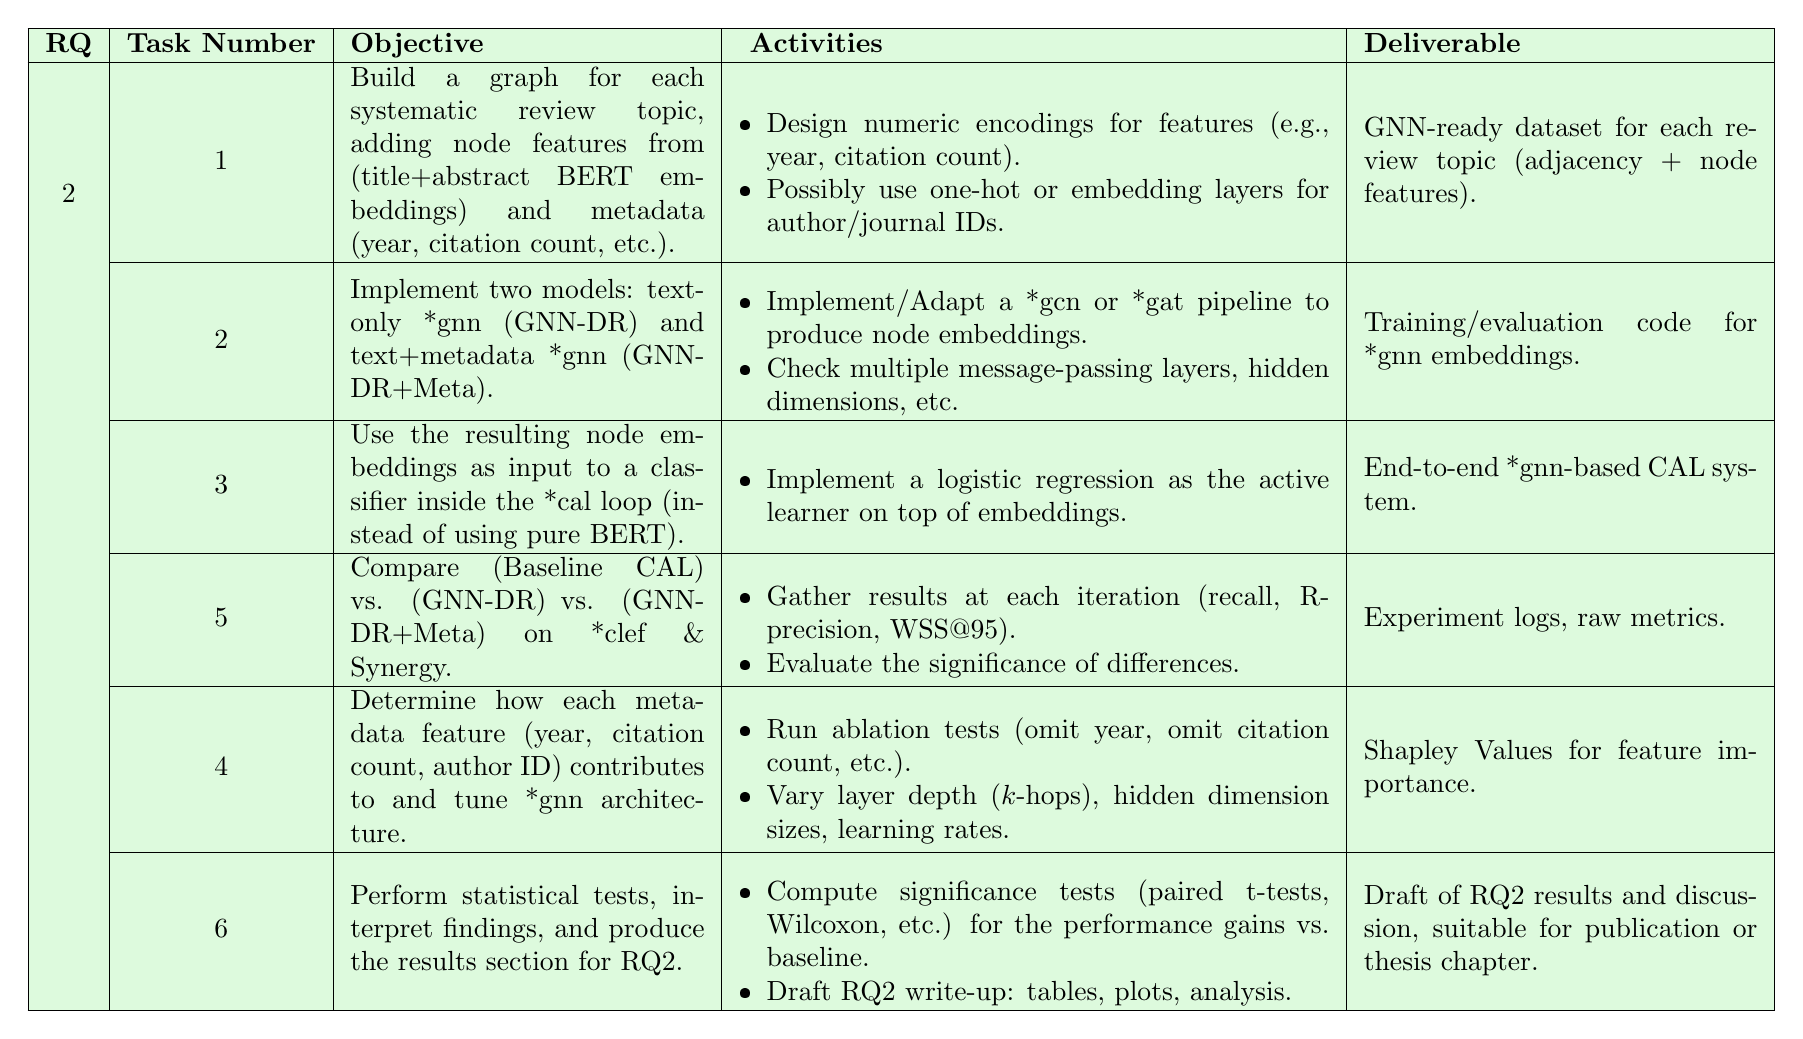
\begin{tikzpicture}
\node[fill=lightgreen, fill opacity=0.3, text opacity=1, inner sep=0pt] {

\begin{tabular}{|c|c|m{4.5cm}|m{7.5cm}|m{5.0cm}|}
\hline
\textbf{RQ} & \textbf{Task Number} & \textbf{Objective }&\textbf{ Activities} & \textbf{Deliverable} \\
\hline
\multirow{3}{*}{2} 
  & 1 &  Build a graph for each systematic review topic, adding node features from (title+abstract BERT embeddings) and metadata (year, citation count, etc.). & 
  \vspace{1em}
      \begin{itemize}[nosep, leftmargin=*]
          \item Design numeric encodings for features (e.g., year, citation count).
          \item Possibly use one-hot or embedding layers for author/journal IDs.
      \end{itemize}
  & GNN-ready dataset for each review topic (adjacency + node features). \\
\cline{2-5}
  & 2 &  Implement two models: text-only \gls*{gnn} (GNN-DR) and text+metadata \gls*{gnn} (GNN-DR+Meta). & 
  \vspace{1em}
      \begin{itemize}[nosep, leftmargin=*]
          \item Implement/Adapt a \gls*{gcn} or \gls*{gat} pipeline to produce node embeddings.
          \item Check multiple message-passing layers, hidden dimensions, etc.
      \end{itemize}
  & Training/evaluation code for \gls*{gnn} embeddings. \\
\cline{2-5}
  & 3 &  Use the resulting node embeddings as input to a classifier inside the \gls*{cal} loop (instead of using pure BERT). & 
  \vspace{1em}
      \begin{itemize}[nosep, leftmargin=*]
          \item Implement a logistic regression as the active learner on top of embeddings.
      \end{itemize}
  &  End-to-end \gls*{gnn}-based CAL system. \\
\cline{2-5}

\cline{2-5}
  & 5 &  Compare (Baseline CAL) vs. (GNN-DR) vs. (GNN-DR+Meta) on \gls*{clef} \& Synergy. & 
  \vspace{1em}
      \begin{itemize}[nosep, leftmargin=*]
          \item Gather results at each iteration (recall, R-precision, WSS@95).
          \item Evaluate the significance of differences.
      \end{itemize}
  &  Experiment logs, raw metrics. \\
\cline{2-5}
& 4 &  Determine how each metadata feature (year, citation count, author ID) contributes to and tune \gls*{gnn} architecture. & 
  \vspace{1em}
      \begin{itemize}[nosep, leftmargin=*]
          \item Run ablation tests (omit year, omit citation count, etc.).
          \item Vary layer depth ($k$-hops), hidden dimension sizes, learning rates.
      \end{itemize}
  &  Shapley Values for feature importance. \\
\cline{2-5}
  & 6 & Perform statistical tests, interpret findings, and produce the results section for RQ2. & 
  \vspace{1em}
      \begin{itemize}[nosep, leftmargin=*]
          \item Compute significance tests (paired t-tests, Wilcoxon, etc.) for the performance gains vs. baseline.
          \item Draft RQ2 write-up: tables, plots, analysis.
      \end{itemize}
  & Draft of RQ2 results and discussion, suitable for publication or thesis chapter. \\
\cline{2-5}
\hline
\end{tabular}
};
\end{tikzpicture}
\caption{Specific task details for RQ 2.}
\label{tab:taskoverview_rq2}
\end{sidewaystable}


\begin{sidewaystable}[htbp]
\centering
\small
\setlength{\extrarowheight}{2pt} % extra spacing between rows
\renewcommand{\arraystretch}{1.2} % increase overall row height

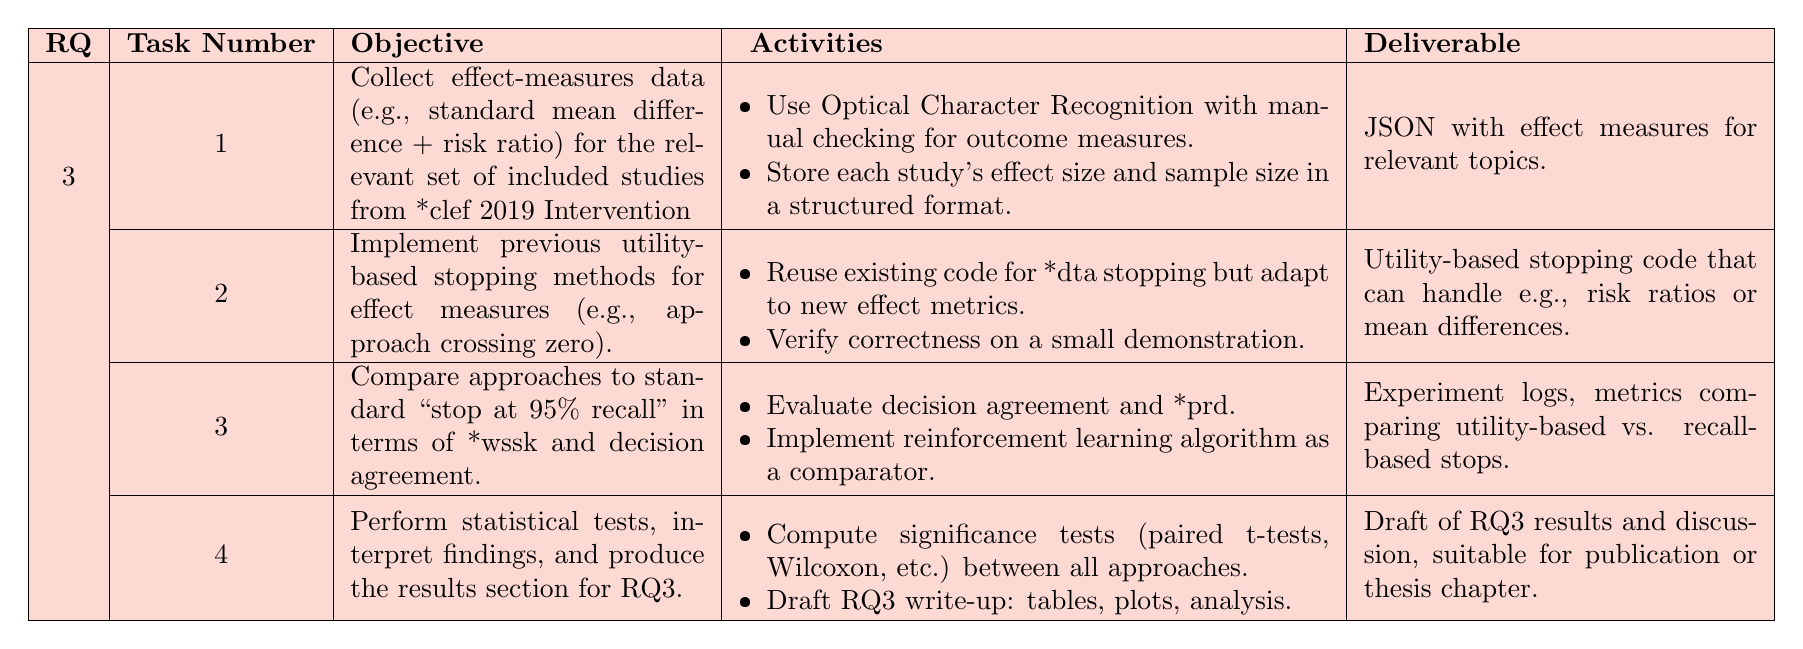
\begin{tikzpicture}
\node[fill=salmon, fill opacity=0.3, text opacity=1, inner sep=0pt] {

\begin{tabular}{|c|c|m{4.5cm}|m{7.5cm}|m{5.0cm}|}
\hline
\textbf{RQ} & \textbf{Task Number} & \textbf{Objective }&\textbf{ Activities} & \textbf{Deliverable} \\
\hline
\multirow{3}{*}{3} 
  & 1 &  Collect effect-measures data (e.g., standard mean difference + risk ratio) for the relevant set of included studies from \gls*{clef} 2019 Intervention & 
  \vspace{1em}
      \begin{itemize}[nosep, leftmargin=*]
          \item Use Optical Character Recognition with manual checking for outcome measures.
          \item Store each study’s effect size and sample size in a structured format.
      \end{itemize}
  & JSON with effect measures for relevant topics. \\
\cline{2-5}
  & 2 &   Implement previous utility-based stopping methods for effect measures (e.g., approach crossing zero). & 
  \vspace{1em}
      \begin{itemize}[nosep, leftmargin=*]
          \item Reuse existing code for \gls*{dta} stopping but adapt to new effect metrics.
          \item Verify correctness on a small demonstration.
      \end{itemize}
  & Utility-based stopping code that can handle e.g., risk ratios or mean differences. \\
\cline{2-5}
  & 3 &   Compare approaches to standard ``stop at 95\% recall" in terms of \gls*{wssk} and decision agreement. & 
  \vspace{1em}
      \begin{itemize}[nosep, leftmargin=*]
          \item Evaluate decision agreement and \gls*{prd}.
          \item Implement reinforcement learning algorithm as a comparator.
      \end{itemize}
  & Experiment logs, metrics comparing utility-based vs. recall-based stops. \\
\cline{2-5}
  & 4 & Perform statistical tests, interpret findings, and produce the results section for RQ3. & 
  \vspace{1em}
      \begin{itemize}[nosep, leftmargin=*]
          \item Compute significance tests (paired t-tests, Wilcoxon, etc.) between all approaches.
          \item Draft RQ3 write-up: tables, plots, analysis.
      \end{itemize}
  & Draft of RQ3 results and discussion, suitable for publication or thesis chapter. \\
\cline{2-5}
\hline
\end{tabular}

};
\end{tikzpicture}
\caption{Specific task details for RQ 3.}
\label{tab:taskoverview_rq3}
\end{sidewaystable}

In creating this time-line for the PhD several assumptions were made:
\begin{itemize}
    \item \textbf{Holiday Periods:} Two weeks of holiday have been accounted for during the summer and a two-week period over Christmas and New Year. This timeline does not account for additional holidays, which will be determined later.
    \item \textbf{Front-Loaded Research:} The research plan is front-loaded, with significant emphasis placed on the early stages of the project. This approach allows additional literature searching, coding, and experimental setup to be completed in advance, providing a solid foundation for later stages of research, the research questions of which are currently flexible. This strategy also ensures that any necessary adaptations can be made based on early findings, reducing the risk of major delays later in the project. 
    \item \textbf{Research Flexibility:} Breaks are scheduled between work on research questions to allow for adaptation or extension if research questions need to be adjusted. In addition, there is a dedicated period for each of the three research themes before beginning coding or experimental setups. This time is intended for further literature review, acknowledging the rapidly evolving nature of this field. The literature is expected to advance before each research question period starts.
    \item \textbf{Undetermined Research Questions:} A single research period has deliberately been left open, \emph{RQ4}. Depending on the findings of the first three research questions, new research opportunities or developments in the field may emerge that require investigation. Additionally, it could be utilised if there are any delays to this project. 
\end{itemize}


\section{Threat analysis}

Table \ref{tab:risk_matrix} outlines a risk matrix of all potential threats.

\begin{itemize}
    \item \textbf{Research Delays:} Unforeseen challenges in research or coding (e.g., complex research questions, experimental setup issues, or unexpected results requiring further analysis) may cause delays.  An open research question period (\emph{RQ4}) mitigates this risk.
    \item \textbf{Technological advancement:} Rapid technological advancements in the field may render parts of the planned research irrelevant or necessitate a significant change of focus. Ongoing literature review during research question experimentation and implementation mitigates this risk.
    \item \textbf{Publication risks:} 
    The research may not yield publishable results, or the publication process may take longer than anticipated, particularly if revisions are required. Extended gaps between research completion and publication, inherent to the publication system, hinder modifying the research to meet reviewer expectations.
    \item \textbf{Personal and Health Factors:} Extended high-intensity work periods can cause burnout or health problems, impacting the planned schedule. The Gantt chart cannot fully account for extended absences due to illness or other personal factors.
    \item \textbf{Open-ended research questions:} A suitable research area may not be identified by the time the open-ended research questions are reached. However, the author believes this is unlikely, as the amount of research in \gls*{cal} for systematic reviews is limited.
    \item \textbf{Competing time constraints from PGDip:} Concurrent PGDip and PhD requirements will sometimes constrain available time. The author has maintained good time management and believes the schedule is reasonable despite these constraints. In case of conflict, PhD work will take priority over PGDip.
\end{itemize}

\begin{landscape}
\begin{table}[t]
\centering
\footnotesize
\begin{tabular}{|c|c|c|c|>{\raggedright\arraybackslash}p{10cm}|}
\hline
\textbf{Threat} & \textbf{Likelihood (L)} & \textbf{Impact (I)} & \textbf{Risk} & \textbf{Response} \\
\hline
Research Delays & 3 & 4 & 12 & Reduce the number of research questions to mitigate delays. \\
\hline
Technological Advancement & 3 & 3 & 9 & Increase time allocated for additional literature review to stay updated with advancements. \\
\hline
Publication Risks & 3 & 3 & 9 & If results are not deemed valid during the analysis phase, proceed to the next research question without spending time on write-up. \\
\hline
Personal and Health Factors & 2 & 4& 8  & Prioritise health by taking regular breaks and managing workload effectively to avoid burnout. \\
\hline
Open-ended Research Questions & 2 & 3 & 6 & Continuously monitor new publications within the domain to ensure relevant and timely research questions. \\
\hline
Competing Time Constraints (PGDip) & 3 & 3 & 9 & Minimize involvement in PGDip activities where possible to focus on PhD work. \\
\hline
\end{tabular}
\caption{Risk Scoring Matrix for threats to PhD. Responses are provided for medium impact risks.}
\label{tab:risk_matrix}
\end{table}
\end{landscape}

\section{Conclusion}

 This project brings together critical gaps in systematic review automation, such as more sophisticated document representations, inter-document relations, and user-centric stopping rules, to advance \gls*{cal} in medical literature screening. By combining citation information and metadata with modern encoder models and \gls*{gnn}, the planned research aims to systematically reduce the screening burden while preserving near-total recall. Moreover, by exploring utility-based stopping criteria, it seeks to align the screening endpoint with the actual value of additional studies, mitigating the inefficiency of rigid recall thresholds. The proposed investigations—spanning citation-augmented seed sets, \gls*{gnn}-driven metadata integration, and novel stopping heuristics — will be validated on widely used \gls*{clef}-\gls*{tar} and Synergy datasets to ensure robust, reproducible results. Ultimately, this work can potentially reduce costs in performing systematic reviews and bolster decision-making quality in \gls*{ebm}, offering an answer to the issue of the ever-growing volume of biomedical research.


\chapter{Supporting works}
\section{Completed research}

\subsection{Presented research}

\paragraph{Screening Prioritisation Lecture:}
A tutorial was given by the author, along with their supervisor, at the British Computing Society on November 26th, 2024, for the Search Solutions 2024 conference on screening prioritisation\footnote{https://www.bcs.org/membership-and-registrations/member-communities/information-retrieval-specialist-group/conferences-and-events/search-solutions/search-solutions-2024}. A copy of the tutorial has been supplied - see Appendix \ref{app:Screening_Prioritisation}. The tutorial was designed to provide an accessible introduction to screening prioritisation within systematic reviews for an audience of \gls*{ir} practitioners and researchers attending the conference. It was structured as a half-day event, with the author delivering a dedicated hour-long lecture. This lecture aimed to demystify the complexities of systematic review screening and highlight the potential of prioritisation techniques to improve efficiency and reduce workload significantly. Key topics covered included the fundamental screening concepts, the challenges of manual screening in large datasets, and a comprehensive overview of various prioritisation strategies, drawing directly from the literature discussed in Section \ref{sec:screening Priorisation}. The lecture effectively served as a practical guide, offering attendees a clear understanding of the current approaches and the potential impact of screening prioritisation in real-world applications. For the author, this lecture experience provided a way to improve their skills in effectively conveying comprehensive overviews of complex literature to a diverse audience. Furthermore, the interactive nature of the tutorial, including the question and answer session, forced engagement with the audience (from the public to \gls*{ir} specialists) and directly supported the communication and dissemination aspects of their PhD research.

\subsection{Research under peer review}

\paragraph{Utility-Based Stopping Methods:}
This research, submitted to SIGIR 2025 conference~\footnote{https://sigir2025.dei.unipd.it} and currently under peer review, introduces a novel utility-based approach to stopping rules for medical literature screening within \gls*{tar}. A copy of the paper has been supplied - See Appendix~\ref{app:Utility_Based_Stopping_Methods}. Moving beyond traditional recall-based methods, this work focuses on stopping the search process based on the utility of the information retrieved thus far, specifically its value in answering the underlying research question. Several new algorithms were developed, leveraging the statistical concept of moments of a probability distribution: Harmonic Shrinkage, Confidence Boundary, Skewness, Kurtosis, and Multi-Moments. Experiments demonstrated that the Confidence Boundary algorithm achieves high decision agreement with significantly reduced document review compared to target-recall approaches. This research supports this PhD's goal of improving efficiency in the medical screening process by offering a more efficient and user-centric approach, aligning stopping decisions with the actual information needs of the user.

\paragraph{Predicting Article Retractions:}
This research, submitted to the journal Research Integrity and Peer Review\footnote{https://researchintegrityjournal.biomedcentral.com} and currently under peer review, investigates the use of machine learning to predict the retraction of scientific articles. A copy of the paper has been supplied - See Appendix \ref{app:Predicting_article_retractions}. A novel dataset was created by combining information from the Retraction Watch database (containing retracted articles) and the OpenAlex API (an academic publication catalogue). The dataset includes 9,028 articles published between 2000 and 2020, equally split between retracted and non-retracted, and features article metadata, abstracts, and citation metrics. Various machine learning models were trained on this data, including traditional feature-based classifiers (like Gradient Boosting, \gls*{svm}, XGBoost, and Random Forest) and \glspl*{llm} such as \gls*{bert}, BioBERT, Llama 3.2, and Gemma 2. The \gls*{svm} model achieved the highest precision (0.690) for identifying retracted articles, while Llama 3.2-base had the highest overall accuracy (0.682) and recall (0.689 for the retracted class). An ablation study revealed that the publication year was the most influential feature for prediction, followed by the primary topic. Interestingly, the abstract's content was less influential than expected. The dataset and code are made publicly available to facilitate further research. This research supports this PhD's main goal of efficiency by providing tools to reduce the larger work pool identified in the systematic review process.

\section{Ongoing research}

\subsection{CPET project}

A cardiopulmonary exercise test (CPET) is performed before certain anaesthetic procedures, the outcome of which is used to determine the patient's suitability for this procedure. Current approaches use summarised data to generate decision models, whose data are derived from summary values provided by the machine. The machine also records ''breath-by-breath" data measurements, which, while they are the basis for the summary values, are not used by these models. This research project attempts to determine whether using deep neural networks with these ''breath-by-breath" data is superior to the traditional summary-model approach. An National Health Service researcher devised this research.

\textbf{Threat to PhD :} Low. The author is providing coding assistance to this project and will not be involved in the analysis or extensively involved in research write-up outside of the technical side. Coding is largely complete. This is also likely to result in publishable research and will likely be published in medical domain venues, promoting interdisciplinary work.


\section{Research output venues}

A dissemination plan is crucial for any research to have an impact. Therefore, a key focus during this PhD will be publishing in high-ranking, peer-reviewed academic venues. The interdisciplinary nature of this research, spanning \gls*{ir}, \gls*{nlp}, Machine Learning, and Medical Informatics, necessitates targeting a diverse range of conferences and journals. While aiming for top-tier venues, the reality of the publication process means that not all outputs will be accepted at the most prestigious outlets. Furthermore, the choice between a conference or a journal will depend on the nature of the specific research output. A non-exhaustive list of potential output targets, ordered by preference within each category, is presented in Table \ref{tab:venues_detailed_landscape}; all conference impact factors were calculated in 2022~\cite{eickhoff_impact_2023}:

\begin{sidewaystable}[htbp]
  \centering
  \caption{Target Publication Venues}
  \label{tab:venues_detailed_landscape}
  \small
  \begin{tabular}{L{3cm} L{15cm} L{1.5cm} L{1.5cm}}
    \toprule
    \textbf{Category} & \textbf{Venue and Rationale} & \textbf{IF} & \textbf{Freq.} \\
    \midrule
    \multicolumn{4}{l}{\textbf{Primary Targets}} \\
    \midrule
    Conferences &
    \textbf{SIGIR} (Special Interest Group on Information Retrieval)\footnote{\url{https://sigir.org}}: The premier international conference for research on \gls*{ir}, strongly aligned with this PhD's core focus on improving the efficiency of systematic reviews.
    & 19.41 & Annual \\
    &
    \textbf{ACL} (Association for Computational Linguistics)\footnote{\url{https://aclanthology.org/venues/acl}}: A leading conference in NLP, relevant due to the use of language models and text analysis in this research.
    & 25.66 & Annual \\
    \midrule
    Journals &
    \textbf{TOIS} (ACM Transactions on Information Systems)\footnote{\url{https://dl.acm.org/journal/tois}}: A premier journal for \gls*{ir} research, providing an avenue for publishing work on the theoretical and experimental aspects of the proposed methods.
    & 5.4 & Quarterly \\
    &
    \textbf{Journal of Biomedical Informatics}\footnote{\url{https://www.sciencedirect.com/journal/journal-of-biomedical-informatics}}: A leading journal in biomedical informatics, suitable for disseminating research on the application of the developed methods to medical systematic reviews.
     & 4.0 & Monthly \\
    &
    \textbf{TACL} (Transactions of the Association for Computational Linguistics)\footnote{\url{https://transacl.org}}: A top-tier journal for NLP, relevant for publishing in-depth studies on the language modelling aspects of this research.
    & 10.9 & Cont. \\
    \midrule
        \multicolumn{4}{l}{\textbf{Secondary Targets}} \\
    \midrule
    Conferences &
    \textbf{NeurIPS} (Neural Information Processing Systems)\footnote{\url{https://neurips.cc}}: A top-tier ML conference, particularly relevant for the work on \glspl*{gnn} and their application to document representation.
    & 23.27 & Annual \\
    &
    \textbf{ECIR} (European Conference on Information Retrieval)\footnote{\url{https://ecir2025.eu}}: A major European \gls*{ir} conference offering a strong platform for disseminating research within the European research community.
     &  & Annual \\
    &
    \textbf{EMNLP} (Empirical Methods in Natural Language Processing)\footnote{\url{https://aclanthology.org/venues/emnlp/}}: A major NLP conference with an emphasis on empirical methods, aligning with the experimental focus of this PhD.
     &  & Annual \\
     \midrule
    Journals &
   \textbf{Information Processing \& Management}\footnote{\url{https://www.sciencedirect.com/journal/information-processing-and-management}}: A reputable journal covering a wide range of topics in information science, suitable for publishing research on the broader implications of the proposed methods.
    & 7.4 & Bimonthly \\

     &
    \textbf{Artificial Intelligence in Medicine}\footnote{\url{https://www.sciencedirect.com/journal/artificial-intelligence-in-medicine}}:  A specialised journal focusing on AI applications in healthcare, relevant for disseminating work on the medical aspects of systematic review automation.
    & 6.1 & Monthly \\
\midrule
    \multicolumn{4}{l}{\textbf{Preprint Servers}} \\
    \midrule
     & \textbf{arXiv}\footnote{\url{https://arxiv.org}} (cs.IR, cs.CL, cs.LG): Depending on the policies of journals or conferences, publishing preprints is possible. &  &  \\
     \midrule
    \multicolumn{4}{l}{\textbf{Other Dissemination Channels}} \\
    \midrule
        & \textbf{University of Sheffield's \gls*{cdt} Conferences}\footnote{\url{https://slt-cdt.sheffield.ac.uk/annual-conference}}:  Provides opportunities to present research and receive feedback. &  & Annual\\
    \bottomrule
  \end{tabular}
\end{sidewaystable}


The specific choice of output target will be determined based on the nature and maturity of the research findings and how well it aligns with the output venue (and not \emph{solely} by impact factor). The decision to submit to a conference or journal will be guided by factors such as the depth of the study, the extent of experimental validation, and the desired speed of dissemination. As stipulated by \gls*{ukri} funding, all research outputs will be in open-access venues. Article publishing charges, when applicable, will be paid for with the \gls*{ukri} grant. Conference Fees will be paid for with the author's enhanced research stipend.  

\section{Doctoral development programme activities}

The fulfilment of the Doctoral Development Programme has been achieved as the author is part of the \gls*{cdt} in Speech and Language Technologies and their Applications. The training provided as part of the PhD with integrated PGDip replaces the university's standard Doctoral Development Programme, and no further activities are required beyond that included in the \gls*{cdt}\footnote{https://sites.google.com/sheffield.ac.uk/slt-cdt-handbook/the-centre}.

\section{Training needs analysis}

A training needs analysis was carried out and agreed with my supervisor - see Appendix \ref{app:tna}.

\printbibliography[title={References}]

\appendix
\appendixpage 

\chapter{British Computing Society tutorial on screening prioritisation}
\includepdf[pages=-]{Confirmation Review/supporting_work/Screening Prioritisation.pdf}
\label{app:Screening_Prioritisation}

\chapter{Predicting Article Retractions}
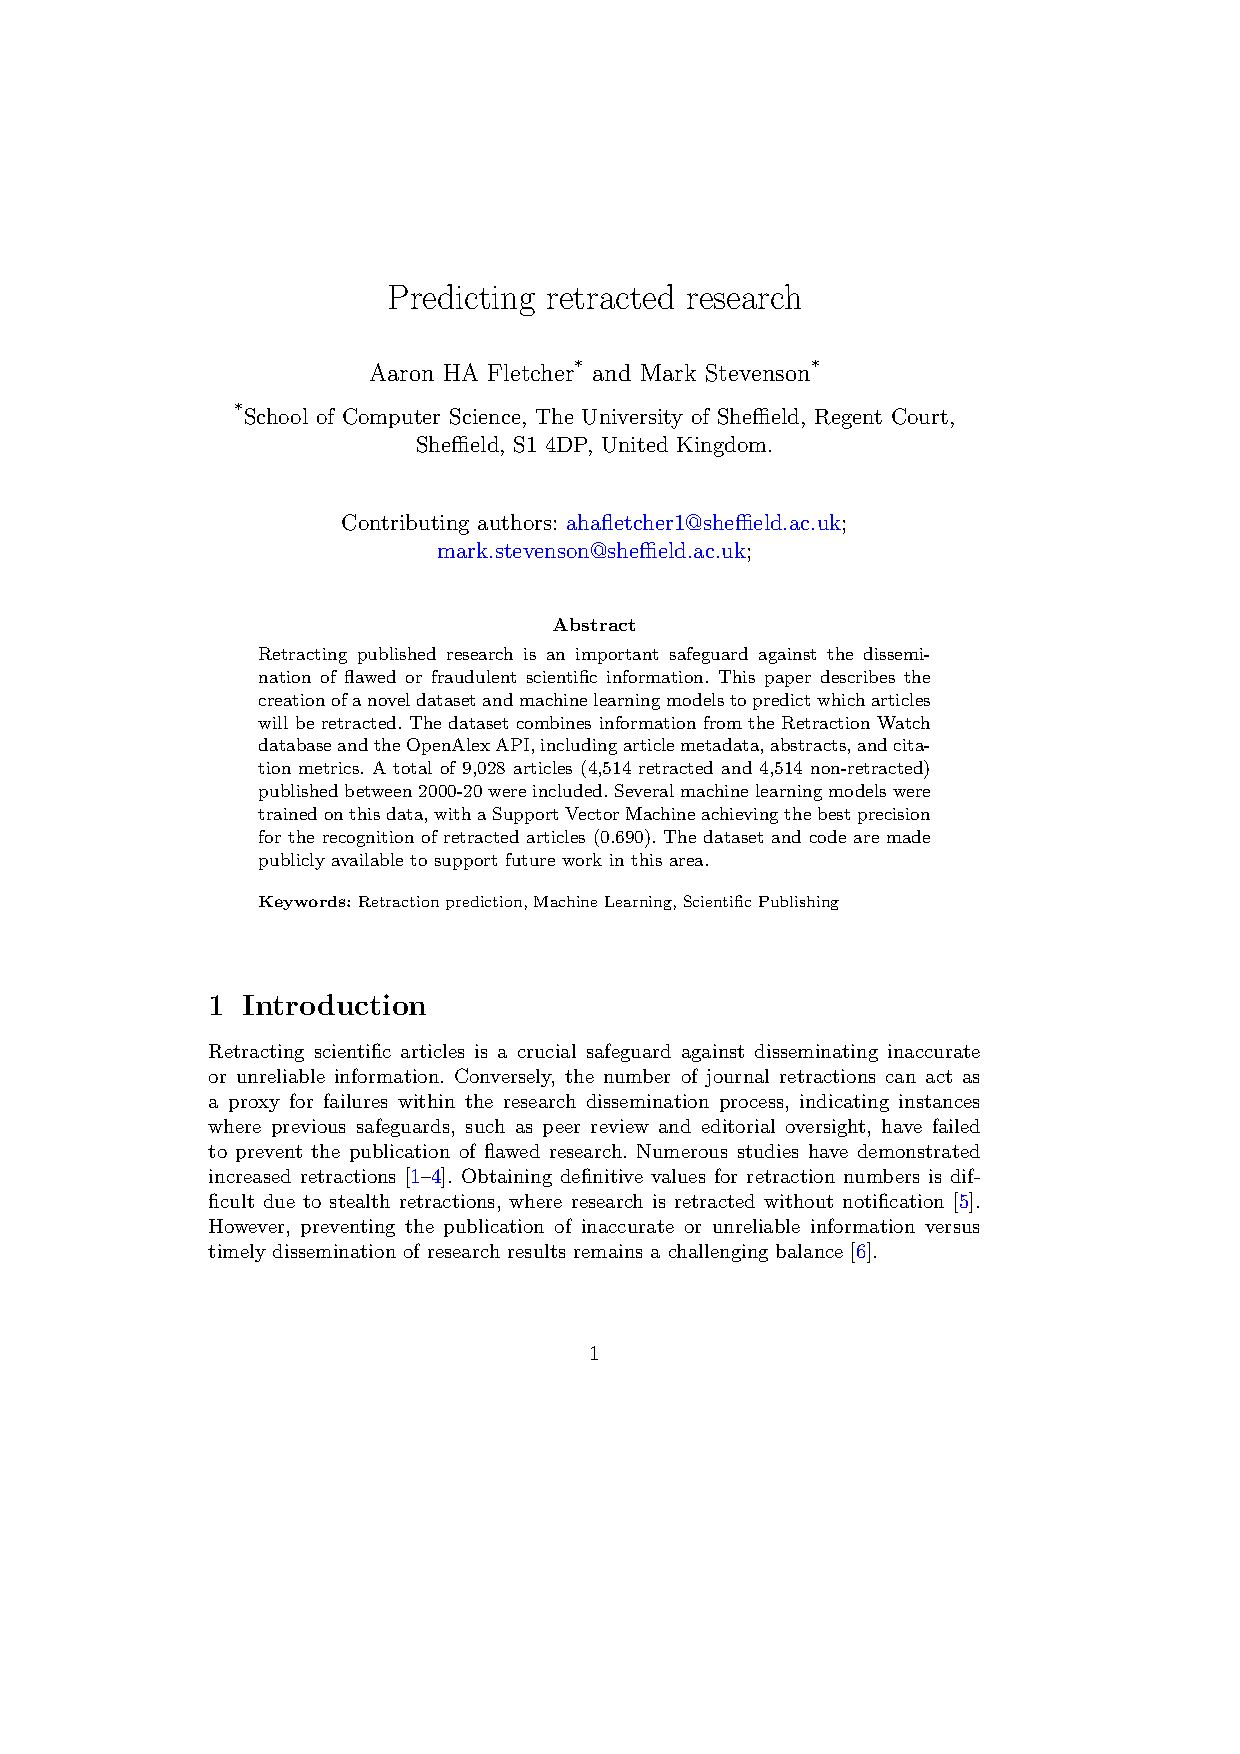
\includepdf[pages=-]{Confirmation Review/supporting_work/Predicting_Article_Retractions.pdf}
\label{app:Predicting_article_retractions}

\chapter{Utility-Based Stopping Methods}
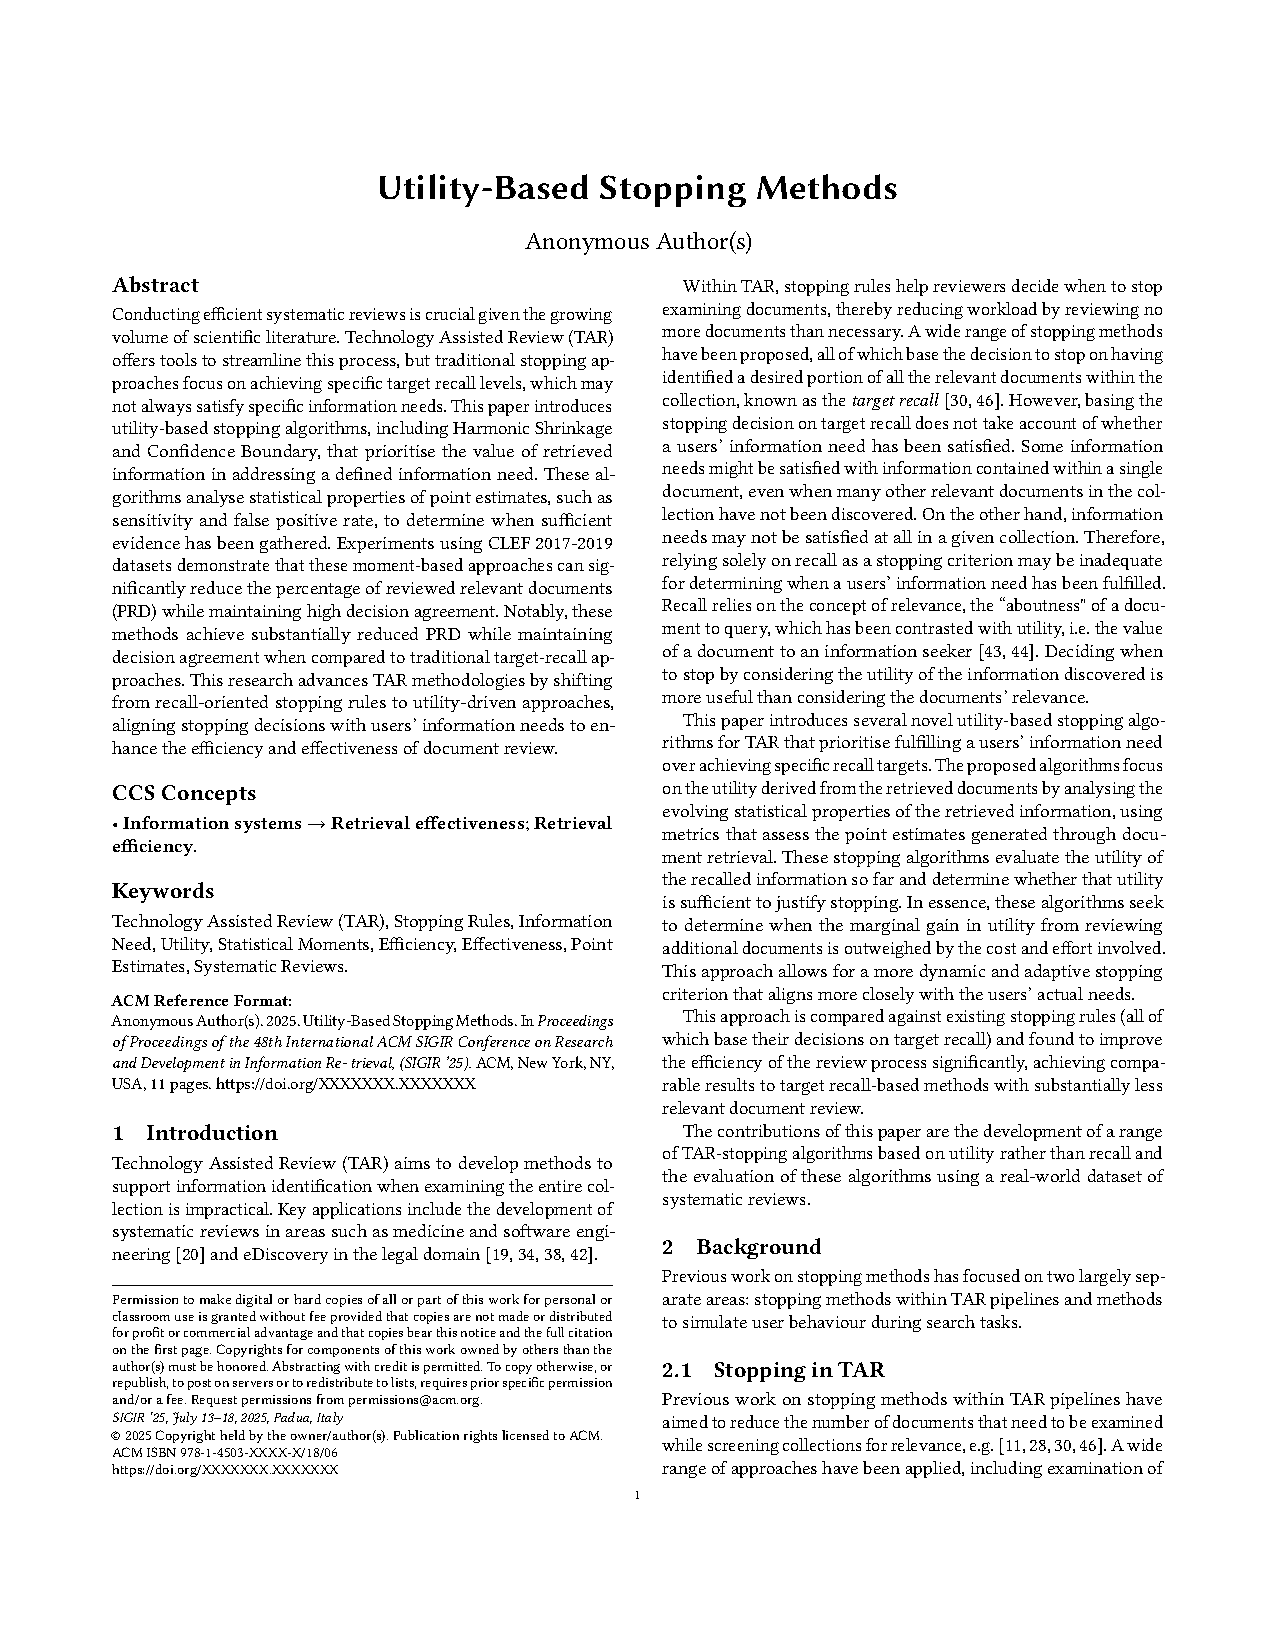
\includepdf[pages=-]{Confirmation Review/supporting_work/Utility_Based_Stopping_Methods.pdf}
\label{app:Utility_Based_Stopping_Methods}

\chapter{Data Management Plan}\label{app:dmp}

\includepdf[pages=-]{Confirmation Review/supporting_work/dmp.pdf}

\chapter{Training Needs Analysis}\label{app:tna}

\includepdf[pages=-]{Confirmation Review/supporting_work/tna.pdf}

\end{document}

